% 文档类(模板)
\documentclass[%
  type = bachelor,  % 本科论文(设计)
  % oneside,        % 单面模式
  twoside,          % 双面模式(openany)
]{nwafuthesis}
% 导言区

% 将需要载入的宏包统一在settings/package.tex中进行管理
% 请按自己的论文排版需求,加载需要的宏包

% TikZ绘图宏包
\usepackage{tikz}
% 卧图卧表宏包
\usepackage{lscape}
% 引号宏包
\usepackage{csquotes}
% 子图表宏包
\usepackage{subcaption}
% 双语标题宏包
\usepackage{bicaption}
% 合并表格行宏包
\usepackage{multirow}
% csv数据处理宏包
\usepackage{datatool}
% 单位符号宏包
\usepackage{siunitx}
% 跨页长表格宏包
\usepackage{longtable}
% 三线表宏包
\usepackage{booktabs}
% 新一代表格排版宏包
\usepackage{tabularray}
% 表格注释说明宏包
\usepackage{threeparttable}
% 带边框小页环境
\usepackage{boxedminipage2e}
\usepackage{float}
\usepackage{multirow}
\usepackage{makecell}

%%% Local Variables:
%%% mode: latex
%%% TeX-master: "../main.tex"
%%% End:

% 将必要的设置统一在settings/format.tex中进行管理
% ==============LaTeX命令排版命令(排版示例文档时使用)========================

\newcommand\cs[1]{\texttt{\textbackslash#1}}
\newcommand\pkg[1]{\texttt{#1}\textsuperscript{PKG}}
\newcommand\env[1]{\texttt{#1}}
\newcommand{\note}[1]{{%
  \color{black}{\bfseries 注意:}\emph{#1}}}
%% ==================================================

% 设置插图目录
\graphicspath{{./figs/},{./logo/}}
%% ==================================================

% 引入tabularray的booktabs库
\UseTblrLibrary{booktabs}

%% 自定义相关的名称宏命令
%% ==================================================
% 西北农林科技大学各单位名称
\newcommand{\nwsuaf}{西北农林科技大学}
\newcommand{\cie}{信息工程学院}
\newcommand{\ca}{农学院}
\newcommand{\cpp}{植物保护学院}
\newcommand{\chc}{园艺学院}
\newcommand{\cast}{动物科技学院}
\newcommand{\cvm}{动物医学院}
\newcommand{\cf}{林学院}
\newcommand{\claa}{风景园林艺术学院}
\newcommand{\cnre}{资源环境学院}
\newcommand{\cwrae}{水利与建筑工程学院}
\newcommand{\cmee}{机械与电子工程学院}
\newcommand{\cfse}{食品科学与工程学院}
\newcommand{\celg}{葡萄酒学院}
\newcommand{\clsc}{生命科学学院}
\newcommand{\cst}{理学院}
\newcommand{\ccp}{化学与药学院}
\newcommand{\cem}{经济管理学院}
\newcommand{\cm}{马克思主义学院}
\newcommand{\chsd}{人文社会发展学院}
\newcommand{\dfl}{外语系}
\newcommand{\iec}{创新实验学院}
\newcommand{\ci}{国际学院}
\newcommand{\dpe}{体育部}
\newcommand{\cvae}{成人教育}
\newcommand{\iswc}{水土保持研究所}

%%% Local Variables:
%%% mode: latex
%%% TeX-master: "../main.tex"
%%% End:


% 编写测试文档用到的两个宏包,若不需要,可能删除
% 中文乱数假文宏包
\usepackage{zhlipsum}
% 最小工作示例(MWE)宏包,主要用于插图示例
\usepackage{mwe}

% 排版设置
\nwafuset{
% 论文格式
  style = {
    % font          = times*,           % 选择英文字体(需要安装有该字体,建议自动配置)
    % cjk-font      = adobe,            % 选择中文字体(需要安装有该字体,建议自动配置)
    hyperlink     = color,            % 超链接颜色
    % withchapter = false,            % 章标题是否为章模式(仅本科生需要)
    bib-resource  = {bib/cite.bib}, % 参考文献数据源文件名,注意需要完整路径及后缀名
    anonymous = false,                 % 是否输出盲审格式论文
  },
% 信息录入
  info = {
    grade = {2025}, % 毕业年份(届)
    enroll = {2021}, % 入学年份(级)
    class-id = {4}, % 班级号
    btype = {paper}, % 本科类型(论文/设计)
    % btype = {design},
    title = {摩托车驾乘人员头盔佩戴检测系统设计与实现}, % 中文题目
    title* = {Design and implementation of helmet wearing detection system for motorcycle riders}, % 英文题目
    department = {信息工程学院}, % 学院名称
    major = {计算机科学与技术}, % 专业
    author = {姜明宇}, % 作者中文名称
    supervisor = {耿耀君}, % 指导教师
    cosupervisor = {}, % 协助指导教师
    date = {\datezh}, % 论文提交时间
    student-id = {2021013149}, % 学号
  },
}
% 录入摘要
\nwafuset{
  abstract = {
    abstractfile  = { contents/chap00-abs-zh.tex }, % 中文摘要文件名称,注意需要有.tex后缀名
    abstractfile* = { contents/chap00-abs-en.tex }, % 英文摘要文件名称,注意需要有.tex后缀名
    keywords      = {目标检测, YOLO, 摩托车头盔, 系统开发, 数据可视化}, % 中文关键字列表,注意用英文逗号分隔。
    keywords*     = {Object Detection, YOLO, Motorcycle Helmet, System Development, Data Visualization}, % 英文关键字列表,注意用英文逗号分隔
  },
}

% \nwafuset{style/hyperlink-color = graylevel}

% 正文区(有且只能有一个)
\begin{document}
% 这个命令用来关闭版心底部强制对齐,
% 可以减少不必要的 underfull \vbox 提示,但会影响排版效果
% \raggedbottom

% 由于论文模板中已设计了自动排版封面、摘要、目录等功能,
% 因此,无需手动排版。

% 主体部分是论文的核心
\mainmatter

% 建议采用多文件编译的方式编写论文,
% 比较好的做法是把每一章放进一个单独的 tex 文件里,
% 并在这里用 \include 导入,如:
% 本文件是示例论文的一部分
% 论文的主文件是位于上级目录的 `main.tex`

\chapter{绪论}

\section{研究目的与意义}

在城市化进程加速和生活节奏日益加快的当下,外卖配送、即时出行等需求呈爆发式增长,
摩托车凭借其小巧灵活、通行便利的特性,在全球各地的城市交通体系中占据了愈发重要的地位。
无论是穿梭于大街小巷的外卖骑手,还是追求通勤效率的上班族,都将摩托车视为短途出行的优质选择。
这一市场需求的增长,有力推动了摩托车产业的蓬勃发展,其保有量在全国范围内持续攀升。

随着摩托车数量的急剧增长,涉及摩托车的交通事故也逐渐增多。头盔作为摩托车驾乘人员唯一的保护装置,能够极大减少交通事故给驾乘人员带来的伤害,尽可能地保护驾驶员和乘客的生命安全\cite{hss}。尽管国家出台了强制佩戴头盔的交通法规
来保障骑行者的生命安全,但部分骑行者安全意识淡薄,依旧心存侥幸,不佩戴头盔就上路行驶,如\ref{fig:traffic}。

当前,针对摩托车驾乘人员头盔佩戴情况的监管,主要依赖交警人工检查。然而,我国道路系统错综复杂,
交通流量庞大且情况瞬息万变,交警在维持交通秩序的同时,还要负责检查头盔佩戴情况,
工作负担极为沉重。人工检查不仅效率低下、耗费大量人力物力,而且在复杂路况和密集车流中,
极易出现漏检现象,难以确保监管工作的全面性和准确性。因此,一个摩托车驾乘人员头盔佩戴检测系统对减少人工工作量、提升检测速度和准确度有很大的意义。

\begin{figure}[!htb]
  \centering
  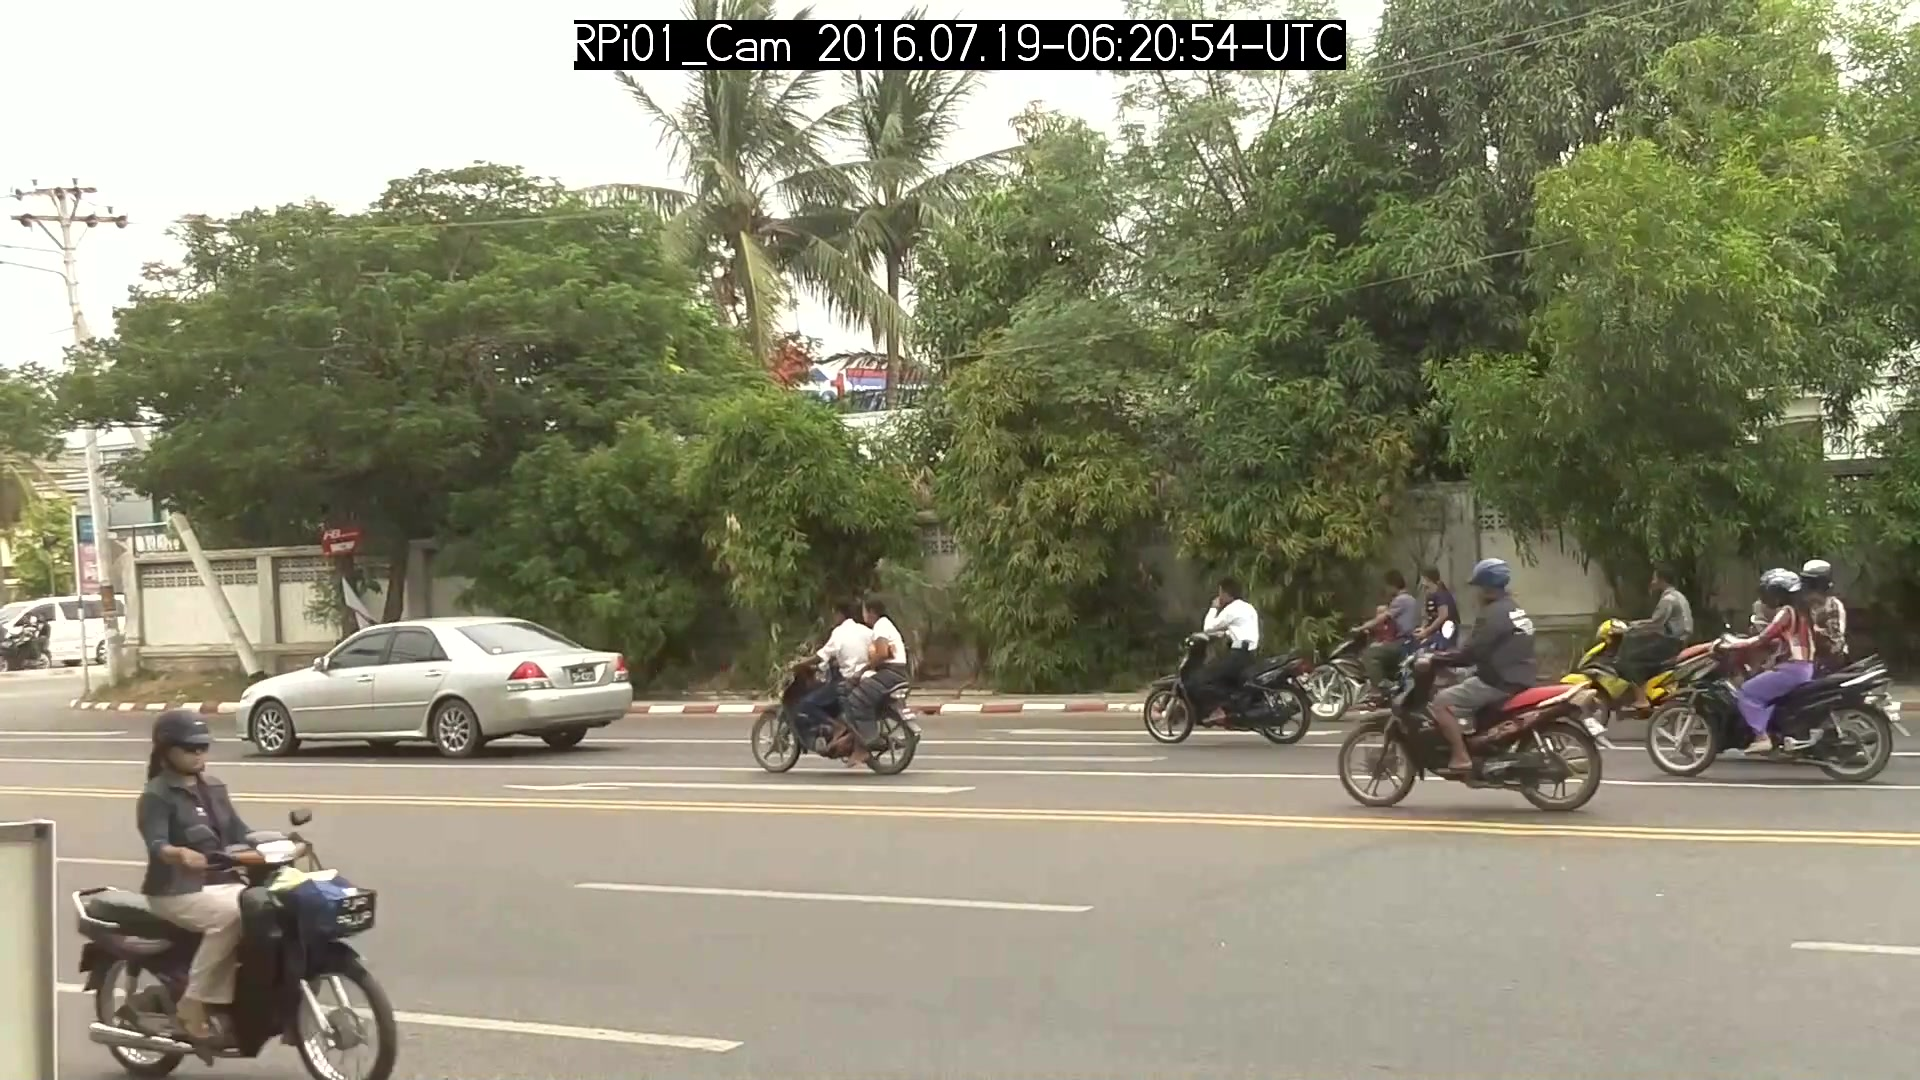
\includegraphics[width=0.85\textwidth]{figs/chap01/traffic}
  \caption{城市道路上摩托车驾乘人员头盔佩戴情况}
  \label{fig:traffic}
\end{figure}
\section{目标检测发展历程}

目标检测是计算机视觉领域的核心任务之一,它的发展历程如\ref{fig:his}所示。

\begin{figure}[!htb]
  \centering
  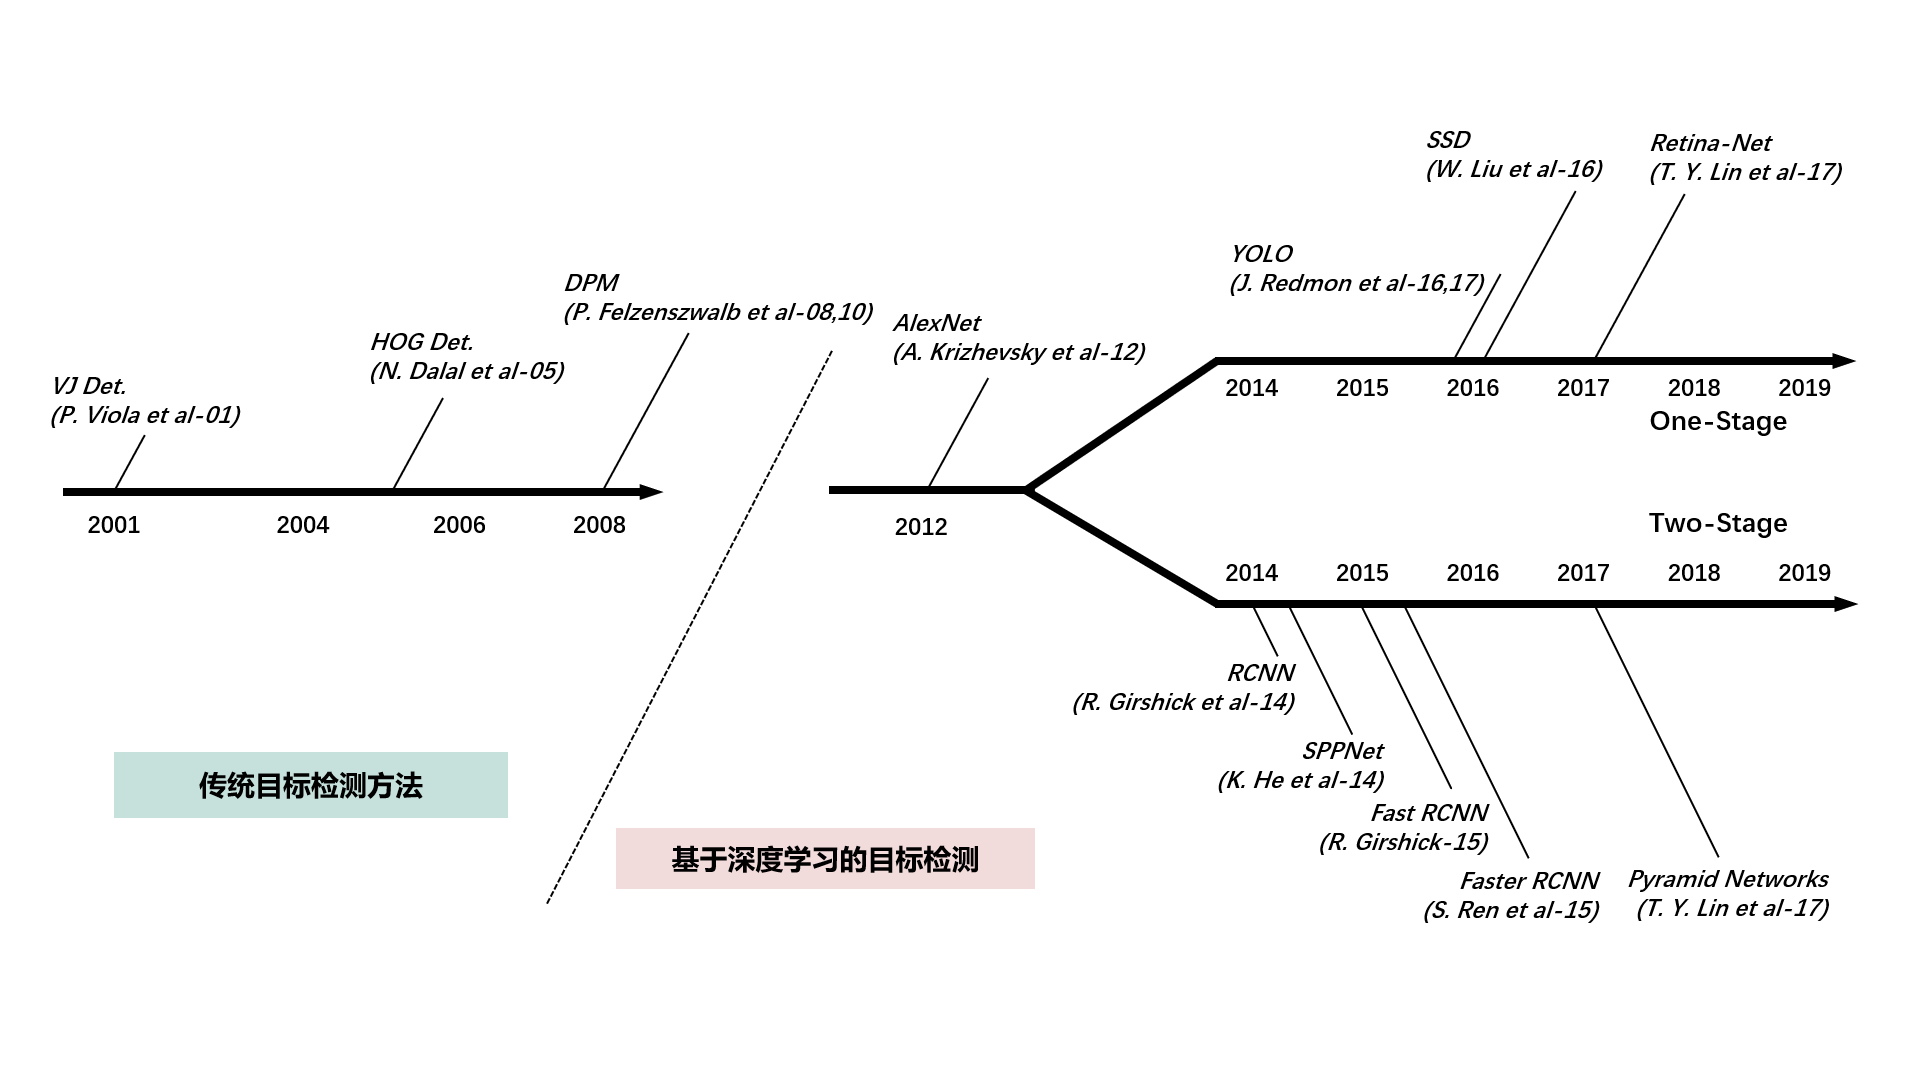
\includegraphics[width=0.9\textwidth]{figs/chap01/his.png}
  \caption{目标检测算法发展历程}
  \label{fig:his}
\end{figure}

\subsection{传统目标检测}
在深度学习兴起之前,目标检测算法高度依赖人工设计特征。受限于图像表示能力,研究者们需要设计复杂的特征表示。这一时期的代表成果深刻影响了后续目标检测技术的发展。

2001年,\textcite{Viola2001}首次在通用场景下实现了无约束的人脸实时检测。相较于同期算法,Viola-Jones(VJ)检测器在保持同等检测精度的前提下,运算速度实现了数十倍乃至数百倍的提升。该检测器运用滑动窗口,对图像内所有尺寸所有位置的窗口进行遍历,判别窗口中是否存在人脸。VJ检测器融合了“积分图像”、“特征选择”以及 “检测级联”技术,大幅提升了检测效率。

Dalal与Triggs于2005年提出方向梯度直方图(HOG)描述器,对当时的尺度不变特征变换和形状语境做出重要改进\cite{Dalal2005}。HOG描述器被设计为在密集的均匀间隔单元网格(区块)上计算,并使用重叠局部对比度归一化方法来提高精度。HOG描述器的主要目标是行人检测,如若要检测不同大小的对象,则需要让HOG检测器在保持检测窗口大小不变的情况下,对输入图像进行多次重设尺寸。

DPM(Deformable Part Models)在目标检测领域具有重要地位,该模型最早由P. Felzenszwalb在2008年提出\cite{Felzenszwalb2008},作为 HOG 检测器的延伸版本,后续经R. Girshick等人不断优化改进\cite{Felzenszwalb2010Cascade}。DPM采用“分而治之”的思想,通过检测对象的各个部件实现目标识别。

\subsection{基于深度学习的目标检测}
2012年,\textcite{alexNet}提出了一种经典的卷积神经网络AlexNet,它的出现对深度学习发展具有里程碑式的意义。基于深度学习的目标检测算法主要分两类:基于回归的一阶段目标检测算法与基于候选区域的两阶段目标检测算法。一阶段算法直接在图像上进行目标检测,将目标检测问题转化为回归问题,直接预测目标的类别和位置,不需要生成候选框,因此检测速度非常快,能够满足实时性要求较高的应用场景,如自动驾驶、视频监控等,代表算法有YOLO系列、SDD等。两阶段算法的第一阶段是生成图像中可能包含目标的候选区域,第二阶段则是对这些候选区域进行分类和边界框回归处理,这种算法检测精度更高,但会牺牲一些检测速度。下面将对两阶段的代表算法R-CNN系列展开介绍,然后详细介绍本文使用到的一阶段的代表算法YOLO系列。

\subsubsection{R-CNN系列算法}
2014年,\textcite{rcnn}提出的R-CNN的思路为:首先通过选择性搜索\cite{selectSearch}算法来提取可能包含目标的候选框,并将候选框调整成固定大小,然后通过AlexNet进行特征提取,最后利用SVM分类器识别每个区域内的目标。尽管R-CNN在目标检测领域实现了突破性进展,但其局限性也较为突出。该模型需对数量众多且相互重叠的候选区域(单张图像通常生成超过2000个候选框)进行特征提取计算,检测速度极慢。同年,\textcite{sppnet}通过引入空间金字塔池化层(SPP),突破了传统CNN需要固定输入尺寸的约束,实现对任意尺寸图像生成固定长度特征表示,将检测速度提升至R-CNN的20倍以上。

2015年,\textcite{fast-rcnn}提出Fast R-CNN检测器,作为对R-CNN和SPPNet的进阶优化成果,其创新地实现了在同一网络配置下同步训练检测器与边界框回归器,降低了训练和推理时间,大大提升了模型的性能。

\textcite{faster-rcnn}提出的Faster R-CNN检测器是第一个端到端的,也是第一个接近实时的深度学习检测器。它引入了RPN(Region Proposal Network)来提升检测速度和性能。RPN用于自动生成候选区域,在性能上要比选择性搜索算法好很多,推动目标检测系统从分散模块逐步整合为统一的端到端学习架构。

\subsubsection{YOLO系列算法}
2016年,\textcite{yolo}提出了YOLO算法,为目标检测任务提供了一种新的解决思路。其核心机制是利用单个卷积神经网络对整幅图像进行处理,将图像分割为多个区域后,直接预测各区域的边界框与对应类别概率,并通过概率加权对边界框进行筛选,经阈值处理后输出高置信度检测结果。与两阶段的R-CNN系列算法相比,YOLO算法在检测速度上有了极大的提升,但也存在一些问题:一是泛化能力弱,难以准确检测训练时未见过的新物体;二是空间约束大,每个网格单元仅预测两个框,不利于处理小目标群;三是定位误差大,经常误判物体位置。

YOLOv2是在YOLOv1发布一年后推出的\cite{yolov2},无论是分类还是检测,YOLOv2都比其前身YOLOv1有了很大的改进。YOLOv2的创新点是提出了一种独特的联合训练算法,该算法能够同时利用检测数据与分类数据对目标检测器进行训练。通过标记检测图像学习目标精确定位,借助分类图像扩展模型识别类别范围、增强鲁棒性。

YOLOv3\cite{yolov3}基于YOLOv2进行改进与创新,实现了性能突破:一方面,YOLOv3修正了YOLOv2的数据加载缺陷,使模型平均精度均值(mAP)提升了两个点;另一方面,YOLOv3引入多尺度预测架构(三尺度特征金字塔)优化跨尺寸目标检测能力,并采用Darknet-53骨干网络,在COCO数据集上实现了精度与速度的平衡。

相较于YOLOv3,YOLOv4\cite{yolov4}在骨干网络和颈部网络两个关键环节进行了创新升级:骨干网络层面,摒弃原有架构,采用CSPDarknet53作为新的骨干网络,通过跨阶段部分网络(CSPNet)策略优化特征提取;颈部结构上,改进空间金字塔池化(SPP)与路径聚合网络(PAN)的引入,进一步强化多尺度特征融合能力。

YOLOv5较YOLOv4在易用性上实现了提升。除了性能上面一些微小的提升之外,YOLOv5基于PyTorch框架重构代码,简化了模型的部署,同时提供了更详尽的多语言文档支持,降低开发门槛。

YOLOv6是YOLO系列中的一次重大演变,由美团视觉团队开发\cite{yolov6}。YOLOv6对YOLOv4和YOLOv5里的PAN拓扑结构进行了强化,借助RepBlocks与CSPStackRep Blocks,更高效地从骨干网络的不同层级聚合特征。除此之外的创新还有:通过硬件感知架构设计与动态训练策略的协同创新,在速度精度平衡与部署效率层面实现突破性进展;核心架构采用EfficientRep主干网络,基于RepVGG重参数化思想构建分层模块化结构,显著提升GPU推理效率;特征融合模块重构为Rep-PAN拓扑,通过重参数化卷积增强跨尺度信息流,并结合解耦式预测头缩减冗余计算。

YOLOv7基于YOLOv6提出了一系列细粒度的改进\cite{yolov7}。提出计划的重新参数化模型,将梯度传播路径概念应用于不同网络层;针对多输出层模型训练,引入由粗到细的引导标签分配的新方法;为对象检测器提出 “扩展” 和 “复合缩放” 方法,有效利用参数和计算。这些改进和优化策略,在不牺牲速度的情况下显著提高了准确率,是YOLO系列的重要进步。

相较于之前的YOLO版本,YOLOv8在准确度和速度方面实现了更优的性能,延续了YOLOv5用户友好的特点,进一步增强了易用性。YOLOv8采用无锚分割Ultralytics head,提升了检测的准确性与速度。YOLOv8 由Ultralytics维护,提供了针对检测、分割、分类和姿势检测等特定任务的多种专用模型。

相较于前代产品,2024年提出的YOLOv9采用全新思路,解决了深度神经网络信息丢失的问题\cite{yolov9}。YOLOv9的核心创新在于两大关键技术:一方面,引入可编程梯度信息(PGI),通过辅助可逆分支完整保留输入信息,为目标函数计算提供充足依据,确保梯度更新更精准有效;另一方面,提出广义高效层聚合网络(GELAN),作为ELAN架构的通用轻量化版本,基于梯度路径规划设计,最大化网络信息流,高效整合特征信息辅助预测。

同为2024年提出的YOLOv10相较于前代作品,刷新了速度与准确度上限,实现了真正的实时检测\cite{yolov10}。YOLOv10的核心创新在于:一是采用NMS-Free检测,基于双重标签分配(一对多和一对一)及一致匹配度量的训练策略,推理时仅用一对一head,提升推理速度、简化部署、增强训练监督;二是运用整体效率-准确度驱动设计,通过轻量级分类head、空间通道解耦下采样和等级引导块设计,在优化模型各组件的同时有效降低计算成本。

2024年9月发布的YOLOv11历经一系列架构改良,聚焦于在无损检测准确性的前提下,全力提升计算效率。YOLO11创新性地引入了C3k2模块与C2PSA块等关键组件。C3k2模块作为跨阶段部分(CSP)瓶颈的高效计算实现,取代了骨干网络和颈部网络中的C2f块。C2PSA块紧跟SPPF模块之后,这种全新的注意力机制,使模型能够更为高效地聚焦于图像内的关键区域,精准识别目标物体。YOLOv11的网络架构将在下一章进行详细介绍。




% 2012 年,AlexNet的提出推动了深度学习在目标识别领域的广泛应用\cite{alexNet}。随后,R - CNN 系列\cite{rcnn}、
% Fast R - CNN\cite{fast-rcnn}、Faster R - CNN\cite{faster-rcnn} 等两阶段检测方法不断改进,显著提升了检测精度和效率。SSD 
% 和 YOLO 系列作为单阶段检测方法,以不同的方式实现了高效的目标检测。其中,YOLO 系列将
% 目标检测转化为回归问题,极大地提高了检测速度,并且后续版本不断优化,加入了多尺度训练等技术,
% 以应对不同尺寸物体的检测需求。

\section{YOLO在交通安全领域的应用}
YOLO系列算法凭借出色的检测速度和准确性在交通安全领域得到了广泛的应用。在车辆检测、行人检测以及道路检测方面均表现出强大的应用潜力。

在车辆检测方面,\textcite{ex1}基于YOLOv8算法,提出了结合Transformer结构全局特征提取能力的模块C2Former代替C2f模块,提升了算法在小目标、遮挡目标等场景下对交通车辆检测的精度。\textcite{ex2}针对雾天场景下的车辆检测需求,引入注意力模块(CBAM、NAM、SimAM)和BiFPN结构优化YOLO-V5s/V5l,并对比了YOLO-V5/V8系列模型的性能,优化了算法在雾天中对车辆的检测性能。

在行人检测方面,\textcite{ex3}基于YOLOv7将ELAN-SA模块与LGA模块相结合,增强了特征提取能力,在遮挡和小目标行人检测方面表现出很强的性能。\textcite{ex4}基于YOLOv11,融合RepConv来改进C3k2模块,设计全新的颈部结构MBFPN,提升行人特征提取与融合能力,提出了复杂场景下的轻量化行人检测算法。

在道路检测方面,\textcite{ex5}提出基于YOLOv8n的轻量化改进算法 EMF-YOLO,通过引入增强型特征融合金字塔EFFPN、可变形注意力机制和多尺度边缘敏感性增强模块MESA等,在提高对道路缺陷检测精度的同时实现了较好的轻量化性能。 

YOLO算法凭借其高效性与准确性,已在交通、工业、医疗等多个领域发挥其作用,提供了精准的实时监测能力,推动各个行业的智能化发展。

\section{研究与设计内容}

在模型训练阶段,主要开展两方面工作:
一是优化数据标注,针对驾驶员及最多三名乘客(训练数据集中,最多 只出现了一名驾驶员携带三名乘客)各自的头盔佩戴情况,细化设置了18个标签,相较于传统二分类标注,能提供更详尽的头盔佩戴信息;二是训练两个关键模型,分别用于识别摩托车驾乘人员的头盔佩戴状态,以及驾驶员id。训练过程中,采用YOLOv11n、YOLOv11s及YOLOv11m三种模型训练来比较效果,并通过调整训练轮次(epoch)优化检测精度。

系统基于浏览器/服务器(B/S)架构开发。B端浏览器为用户提供了两个操作页面,一个是用于上传图片或视频以请求检测的页面,用户可通过该页面发起检测需求;另一个是数据查询页面,用户能从该页面向服务端数据库发送历史检测结果查询请求,还可以对驾驶人、记录时间、记录地点等字段进行过滤。查询得到的结果会以柱状图、折线图等可视化的形式在页面呈现,为后续制定执法策略提供数据支持。S端服务器负责处理浏览器传来的请求,当接收到用户上传的图片或视频后,先利用第一个模型预测图片中的头盔佩戴情况,之后对目标区域进行裁剪,再使用第二个模型检测目标区域的驾驶人员,最后将检测结果保存到数据库中。\ref{fig:source}和\ref{fig:result}表示了输入图片和检测结果。

\begin{figure}[!htb]
  \centering
  \begin{minipage}{0.45\textwidth} % 调整宽度以适应需求,两张图总宽度接近1
      \centering
      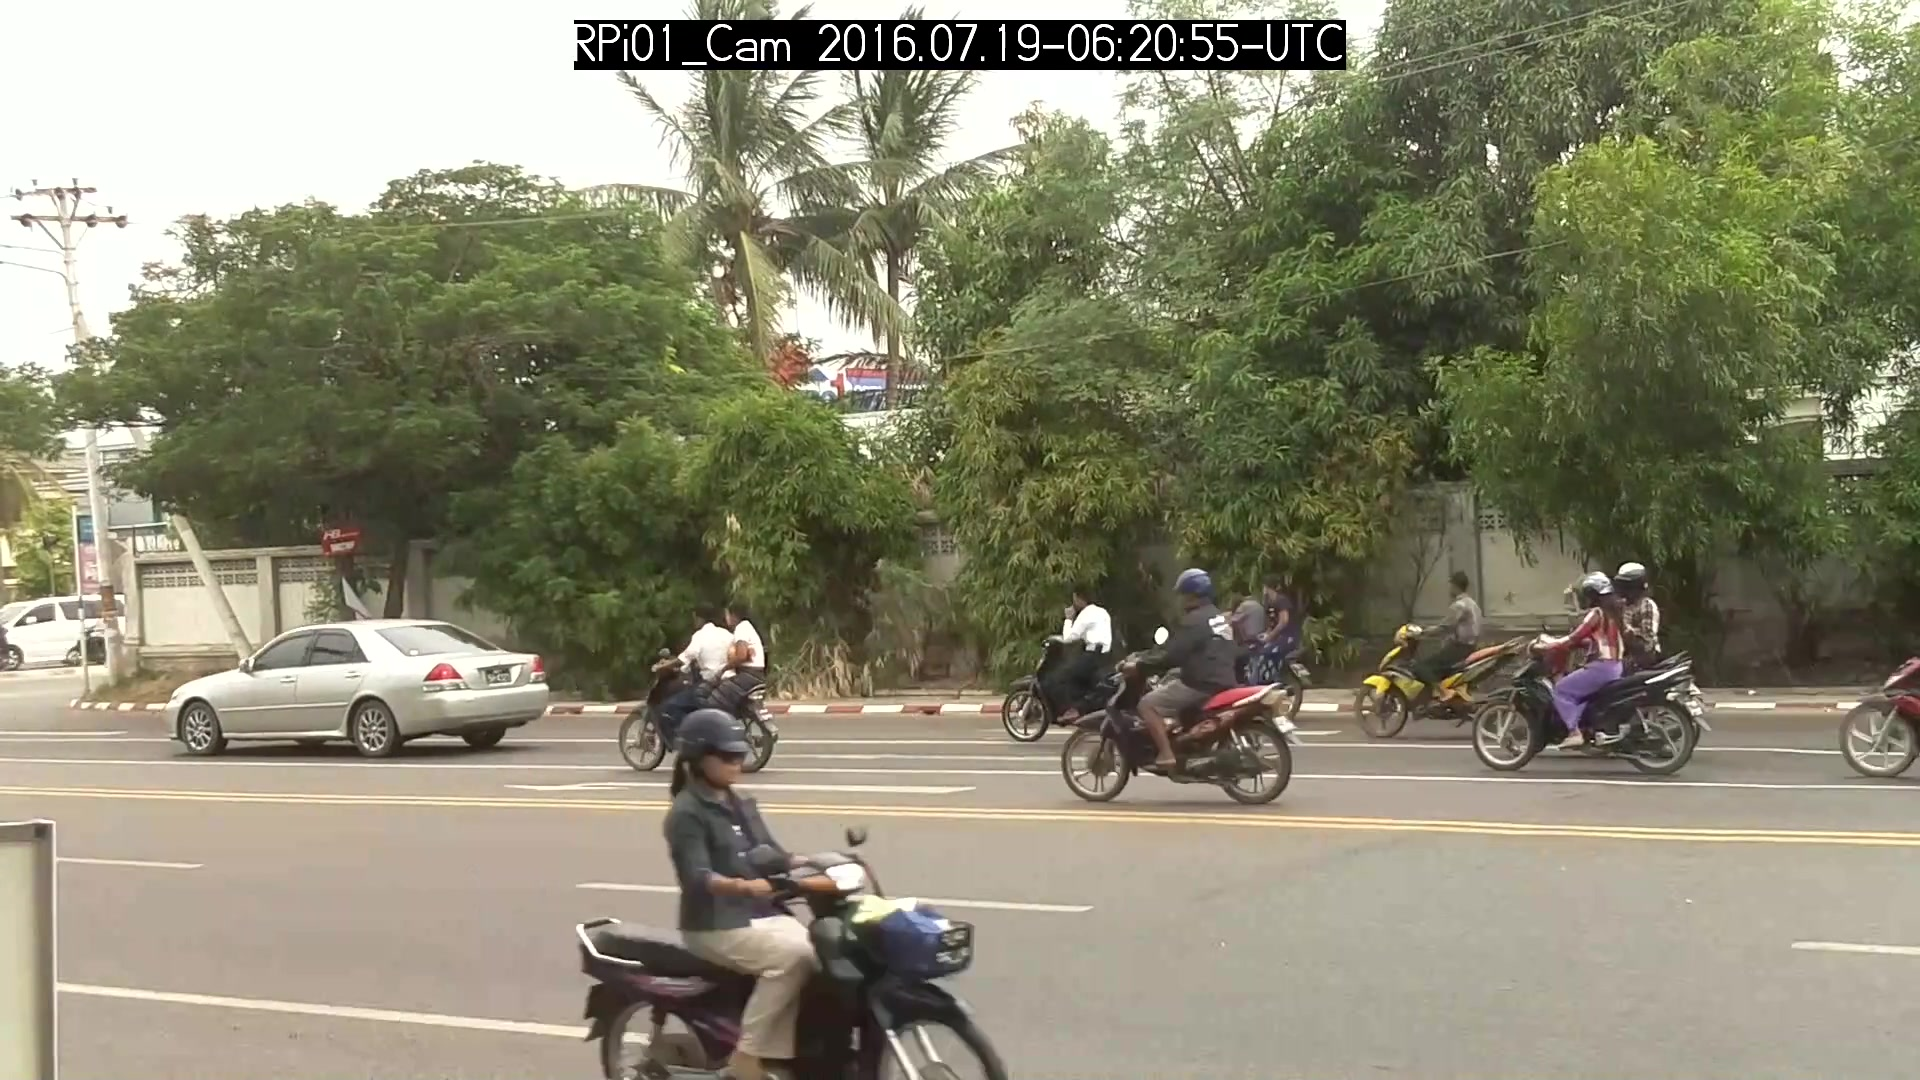
\includegraphics[width=\textwidth]{figs/chap01/source.jpg}
      \caption{选择图片}
      \label{fig:source}
  \end{minipage}
  \hfill % 使两张图片之间保持一定距离
  \begin{minipage}{0.45\textwidth}
      \centering
      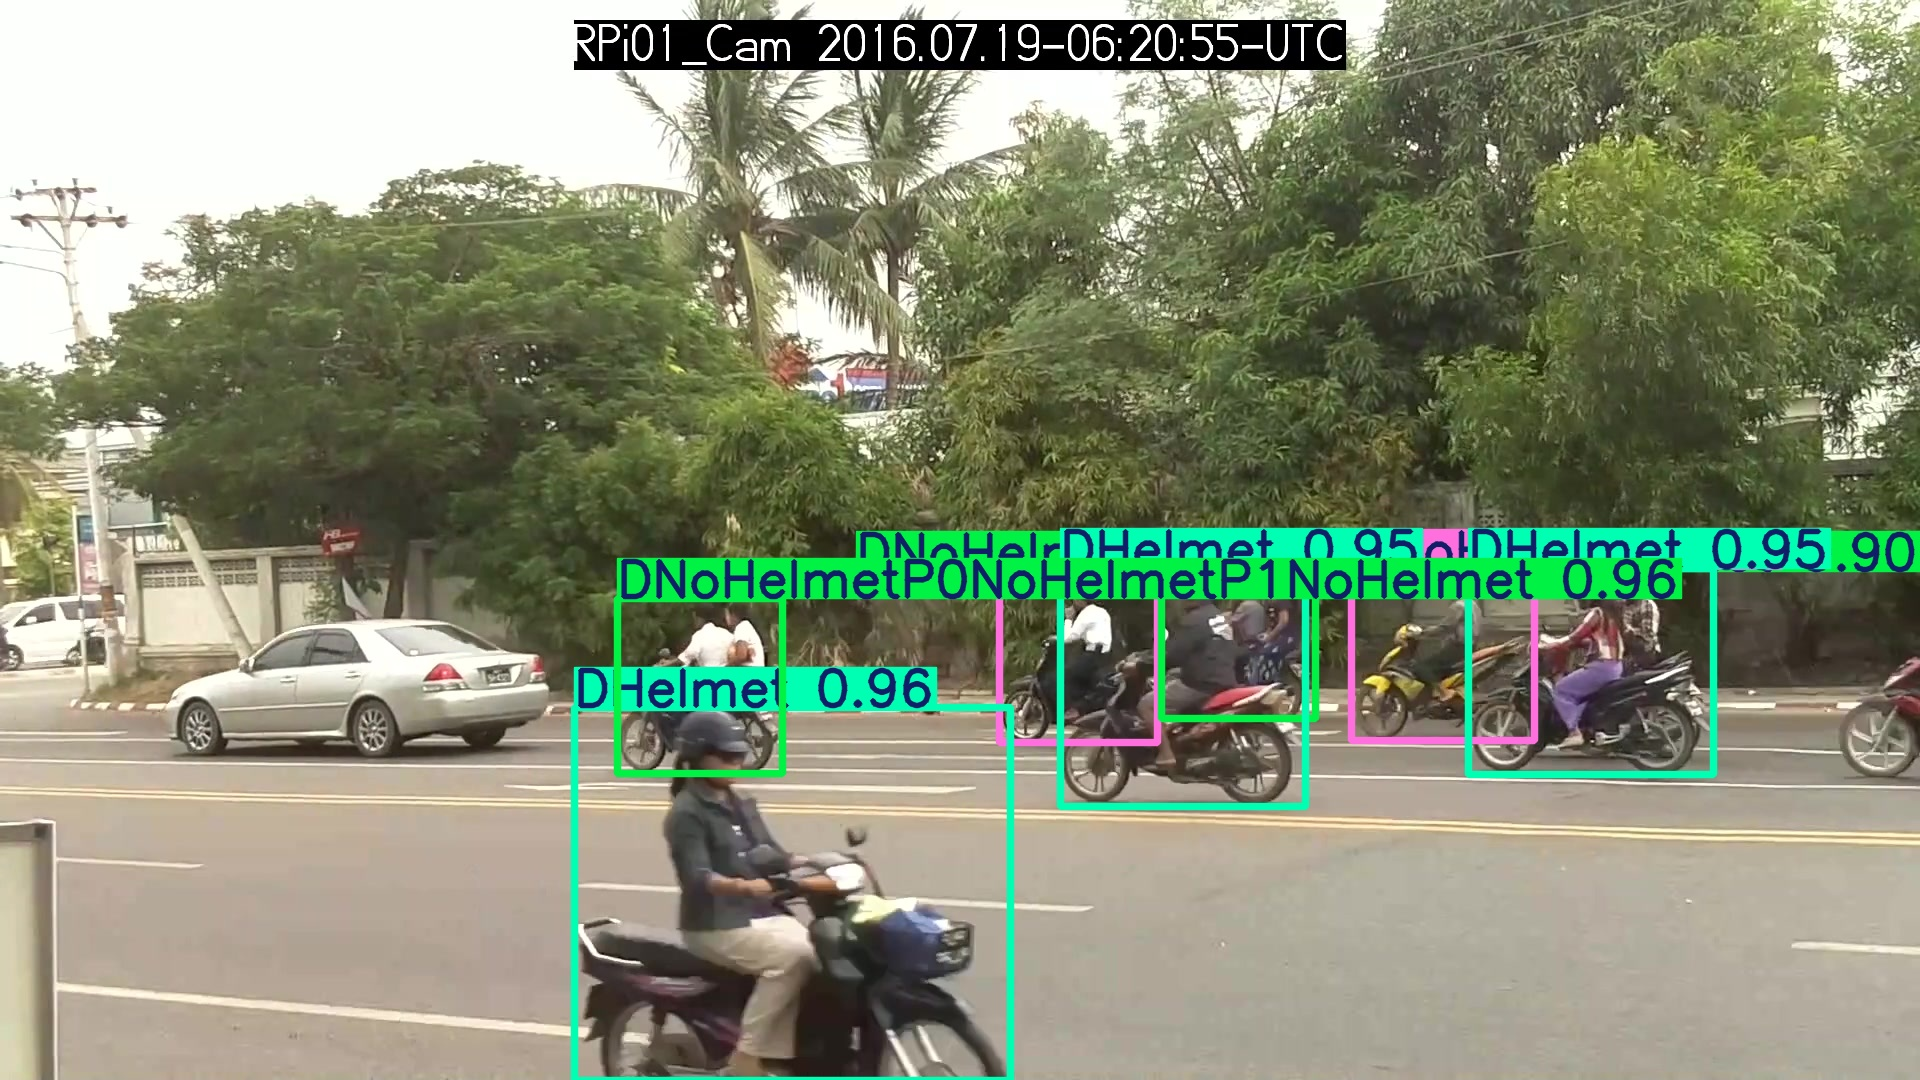
\includegraphics[width=\textwidth]{figs/chap01/result.png}
      \caption{检测结果}
      \label{fig:result}
  \end{minipage}
\end{figure}


\section{章节安排}
本文共包含六个章节,每一章的主要内容如下:

第一章:绪论。本章首先介绍了本文的研究目的与意义,对目标检测的发展历程进行概述,详细介绍了YOLO系列算法的发展过程及其在交通安全领域的应用现状,最后说明了本文的研究内容。

第二章:YOLO算法相关理论。本章主要介绍了YOLOv11算法的网络结构和损失函数。网络结构方面主要介绍主干网络、颈部网络和检测头。损失函数主要介绍边界框回归损失函数、分类损失函数和分布损失函数。

第三章:数据集构建及训练参数设置。本章介绍了本文的数据集来源以及为解决类别不平衡对数据集做的增强处理,分析了增强之后的标签数量分布情况,然后介绍了本文的实验环境和训练参数设置。

第四章:实验结果与分析。本章首先介绍了本文使用到的目标检测模型检测精度和速度两方面的评价指标,展示了YOLOv11n、YOLOv11s和YOLOv11m这三个模型的训练结果,对比分析了上述三个模型的精度、召回率、mAP以及检测速度,总结了各模型适用的场景。

第五章:检测系统的设计与实现。本章主要介绍了检测系统的软件设计与开发过程。从需求分析、系统架构、前端开发和后端开发这四个方面展开。

第六章:总结与展望。本章为本文的最后一张,对本文所做的工作进行总结,并展望目标检测技术在交通安全领域的未来的发展情况。
%%% Local Variables:
%%% mode: latex
%%% TeX-master: "../main.tex"
%%% End:

% 本文件是示例论文的一部分
% 论文的主文件位于上级目录的 `main.tex`

\chapter{YOLO算法理论及数据集预处理}

\section{YOLOv11网络结构}
YOLOv11的网络架构采用骨干网络-颈部网络-检测头的分层设计。骨干网络作为特征提取的基石,引入C3K2模块、SPPF(快速空间金字塔池化)和C2PSA(具有注意力机制的卷积模块)组件,实现了高效的底层特征提取;颈部网络将C2F模块替换为了C3K2模块,提升了特征聚合过程的整体性能,通过C2PSA模块增强了对空间注意力机制的关注;检测头负责生成目标检测和分类的最终预测,它处理从颈部网络传递过来的特征图,最终输出图像中目标的边界框和类别标签。\ref{fig:s}(图像来源:\url{https://zhuanlan.zhihu.com/p/4251780251})展示了YOLOv11的网络结构。
\begin{figure}[!htb]
  \centering
  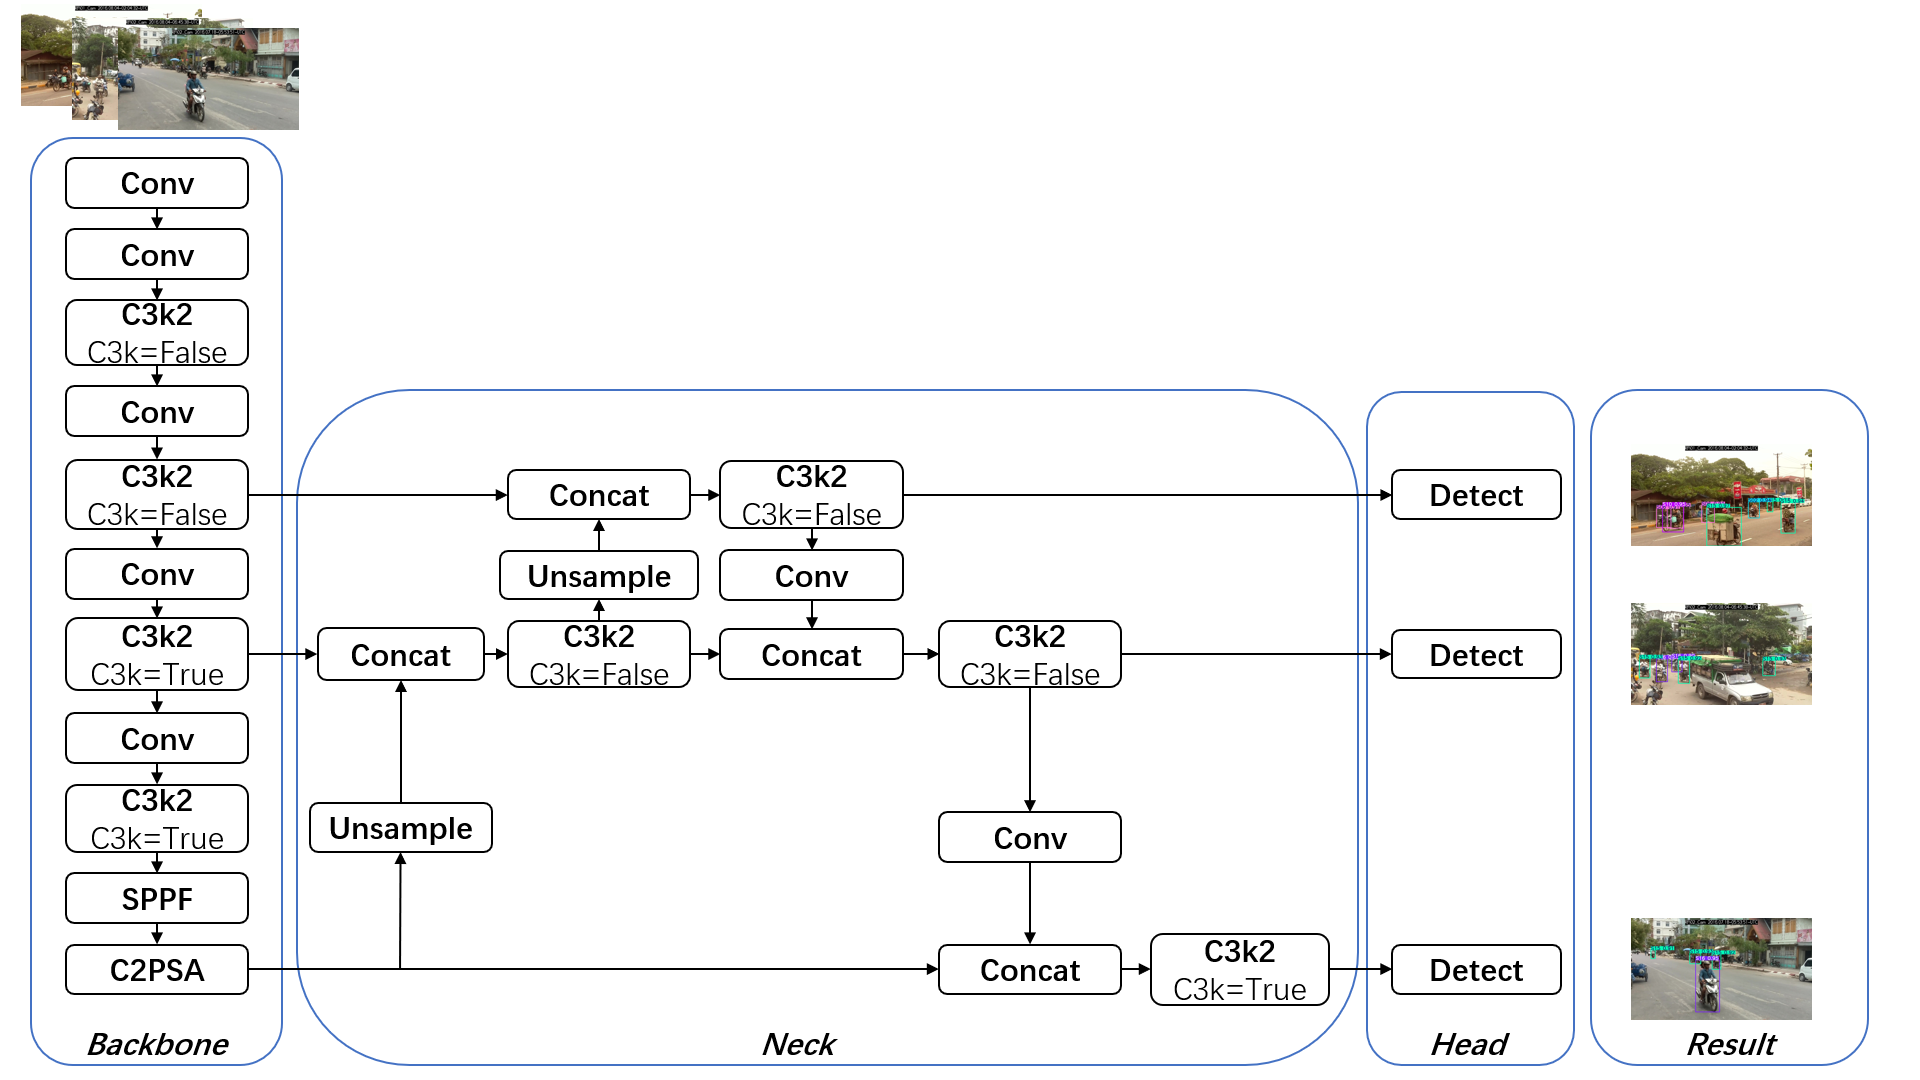
\includegraphics[width=1\textwidth]{figs/chap02/yolov11.png}
  \caption{YOLOv11网络模型}
  \label{fig:s}
\end{figure}

\subsection{骨干网络}
YOLOv11的骨干网络是整个架构的核心特征提取模块,包含Conv、C3K2、SPPF和C2PSA模块。

Conv卷积模块的处理步骤可以概括为数据准备、参数配置、卷积运算和非线性激活四步。Conv模块的输入通常是$(B, C, W, H)$四维张量,$B$表示训练批次;$C$表示数据通道数,彩色RGB图像的通道数为3;$W$表示图像的宽度,$H$表示高度。卷积层的核心参数包括卷积核、步长(stride)、填充(padding),卷积核决定特征提取的局部感知范围,步长控制卷积核滑动间隔以实现下采样,填充通过边界补零调整输出尺寸以及输出通道数。卷积运算这一步将配置好的卷积核应用于输入数据,通过滑动窗口对每个局部区域进行加权求和,实现特征提取。非线性激活应用ReLU、silu等激活函数引入非线性变换,使模型能够学习复杂模式,最终输出处理后的特征图用于后续层的计算。

C3K2模块是早期版本中引入的CSP(Cross Stage Partial) Bottleneck的演变,用来处理骨干网络不同阶段的特征提取。C3K2模块通过分割特征图,并应用一系列较小的(3$\times$3)卷积核进行卷积操作,优化了网络中的信息流,这些卷积比较大的卷积核更快,计算成本更低。与YOLOv8的C2F模块相比,C3K2模块能够以更少的参数提升特征表示能力。
C3K2模块使用C3K模块来处理信息。它在开始和结束时各有一个Conv模块,中间是一系列的C3K模块。将起始Conv模块的输出与最后一个C3K模块的输出进行拼接,并以一个最终的Conv模块结束。这个模块借助CSP结构,致力于在速度和准确性之间保持平衡。
C3K模块的结构与C2F模块类似,但在此模块中不会进行分割操作。输入数据先经过一个卷积模块,随后经过一系列Bottleneck,并以最终的Conv块结束。这三个模块的结构如\ref{fig:c3k}(图像来源:\url{https://medium.com/@nikhil-rao-20/yolov11-explained-next-level-object-detection-with-enhanced-speed-and-accuracy-2dbe2d376f71})所示。

\begin{figure}[!htb]
  \centering
  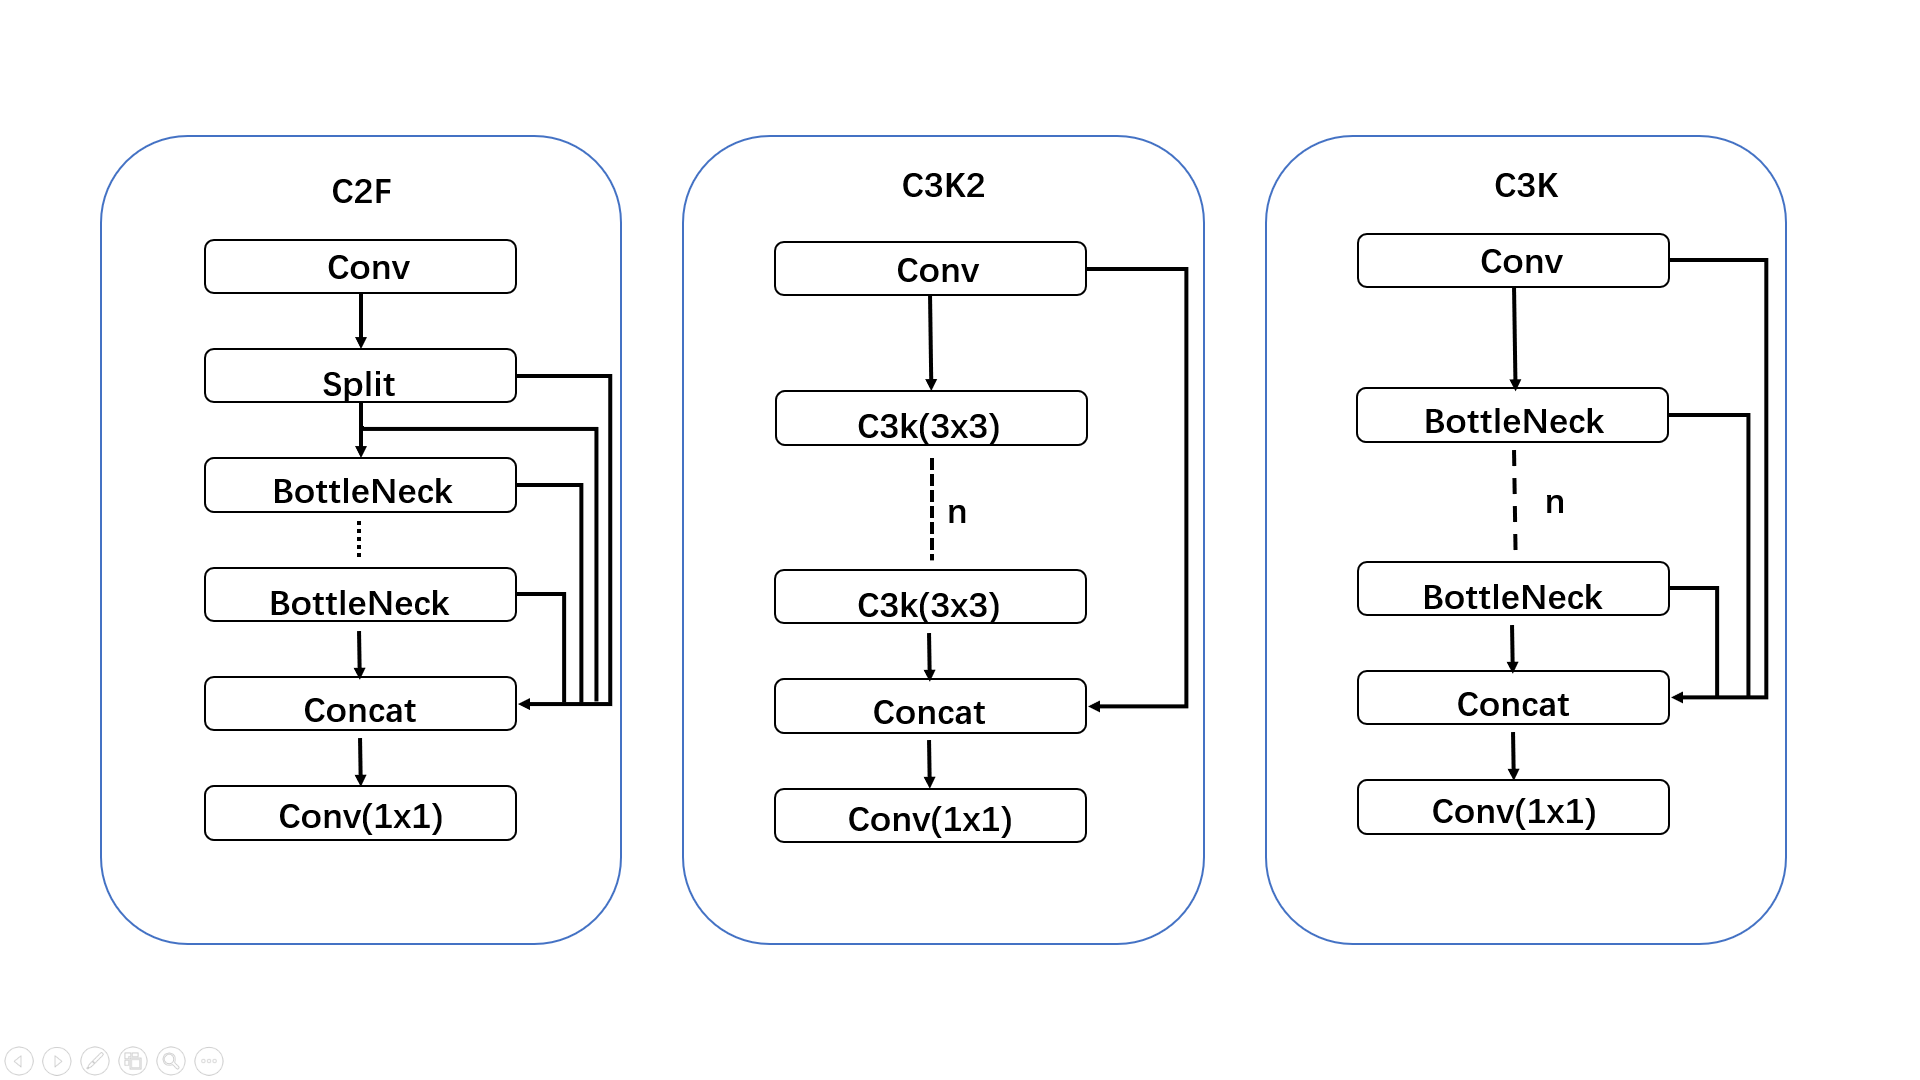
\includegraphics[width=0.9\textwidth]{figs/chap02/c2f.png}
  \caption{C2F和C3K2模块的比较}
  \label{fig:c3k}
\end{figure}

SPPF(Spatial Pyramid Pooling - Fast)模块是对SPP(Spatial Pyramid Pooling)模块的改进,主要用于增强模型对不同尺度目标的检测能力,其结构如\ref{fig:sppf}(图像来源:\url{https://zhuanlan.zhihu.com/p/4251780251})所示。SPPF模块接收C3K2模块输出的特征图,对特征图同时应用多个不同大小的最大池化操作(MaxPool),然后将原始特征图和所有池化后的特征图在通道维度上拼接,形成更丰富的多尺度特征表示,最后通过1×1卷积压缩拼接后的特征通道数,减少计算量。

\begin{figure}[!htb]
  \centering
  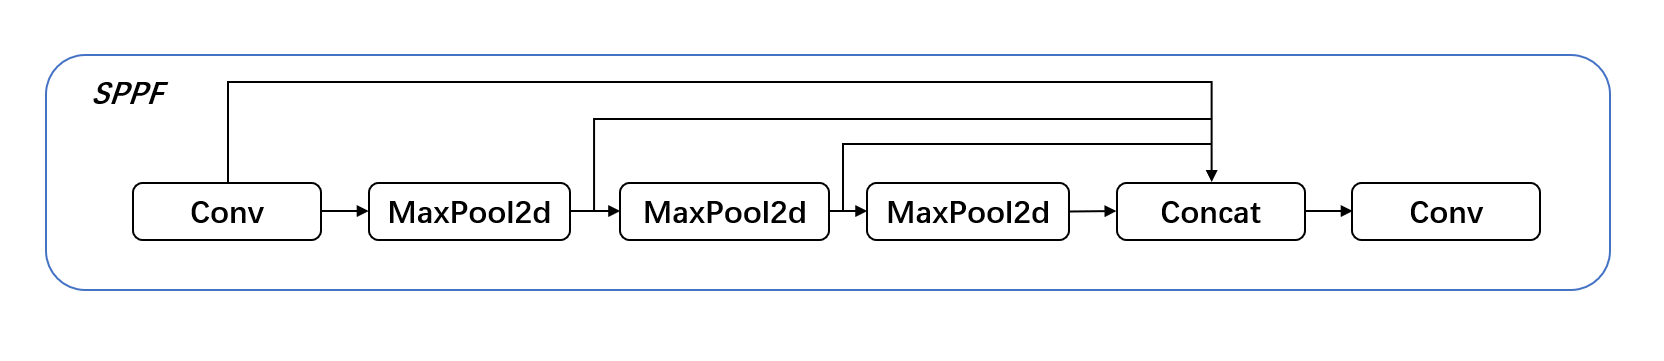
\includegraphics[width=0.9\textwidth]{figs/chap02/sppf.png}
  \caption{SPFF模块结构}
  \label{fig:sppf}
\end{figure}

该模块采用多尺度最大池化核进行特征提取,有效实现对目标多尺度特征的全面表征,通过对不同尺寸池化核获取的特征图进行整合。

C2PSA模块是YOLOv11的一大创新点,该模块结构如\ref{fig:c2psa}(图像来源:\url{https://zhuanlan.zhihu.com/p/4251780251})所示。此模块引入了注意力机制,提高模型对图像中重要区域(例如较小或部分遮挡的对象)的关注。C2PSA模块中的Position-Sensitive Attention封装了对输入张量应用位置敏感注意力和前馈网络的功能,提升了特征提取和处理能力。C2PSA模块采用两个PSA(Partial Spatial Attention)模块,分别处理特征图分支后再拼接,类似C2F模块结构。这种设置在兼顾计算成本与检测精度的同时,让模型聚焦空间信息,使YOLOv11在需关注物体细节以实现精确检测的场景中优于YOLOv8等版本。

\begin{figure}[!htb]
  \centering
  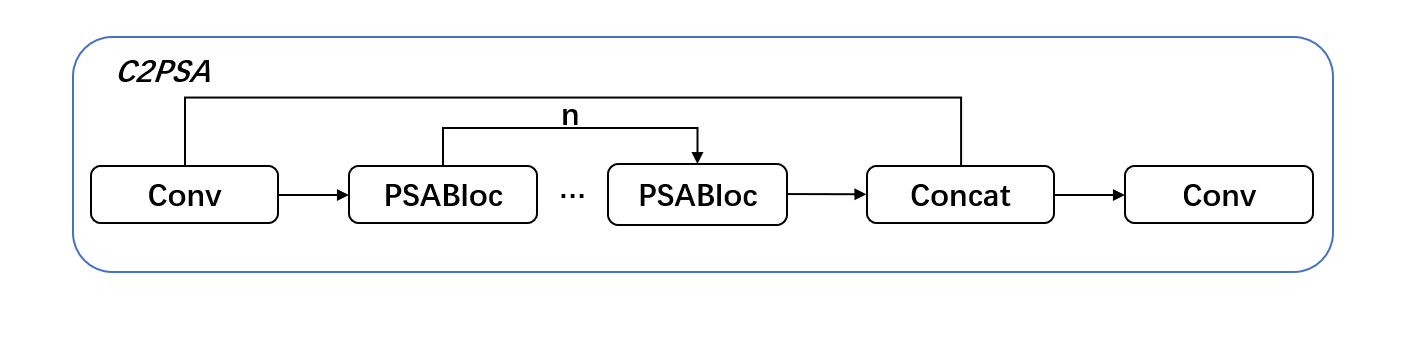
\includegraphics[width=0.9\textwidth]{figs/chap02/c2psa.png}
  \caption{C2PSA模块结构}
  \label{fig:c2psa}
\end{figure}

\subsection{颈部网络}
颈部网络由多个Conv卷积层、C3K2模块、Concat操作和上采样模块组成,并结合了C2PSA机制的优势。

Conv模块对特征图进行卷积运算,一方面可以调整特征图的通道数,使不同特征图在拼接前通道数匹配;另一方面能进一步提取特征,增强特征表达。C3K2模块应用了一系列较小的卷积核,以更少的参数提升特征表示能力。Concat模块沿着通道维度将多个特征图合并在一起,融合不同尺度的特征信息,增加特征的丰富度。
上采样模块通过运用插值等技术手段,实现特征图尺寸的扩充。这一操作的核心目的在于确保特征图维度与其他分支保持一致,借助这种方式,模型得以充分融合多尺度特征信息,提升了模型的检测精度。

颈部网络接收骨干网络不同层级输出的特征图,一些特征图会先经过Unsample上采样操作,使其尺寸与其他待拼接特征图一致,然后再进行Concat拼接。拼接后的特征图,再次经过若干C3K2模块和Conv卷积层,进一步融合与提炼特征。

\subsection{检测头}
与早期的YOLO版本类似,YOLOv11使用多尺度预测头来检测不同大小的对象。头部使用由主干网络和颈部网络生成的特征映射输出三种不同比例(低、中、高)的检测框。
检测头会输出来自三个特征映射(通常来自P3、P4和P5)的预测,对应于图像中的不同尺度级别。这种方法可以确保在更精细的细节(P3)中检测到较小的对象,而在更高级别的特征(P5)中捕获较大的对象​。

\section{YOLOv11损失函数}
YOLOv11的损失函数主要分为:边界框回归损失(BBox Loss)、分类损失(Classification Loss)和分布损失(Distribution Focal Loss, DFL)。

\subsection{边界框回归损失}
边界框回归损失函数为\ref{eq:bbox},$S$ 是网格的大小,
$B$ 是每个网格单元预测的边界框数量,
$1_{ij}^{obj}$ 表示第 $i$ 个网格单元中第 $j$ 个边界框是否负责预测目标。
$x, y$ 是边界框中心点的坐标。
$w, h$ 是边界框的宽度和高度。
$\lambda_{coord}$ 是权重系数,用于平衡不同部分的损失。

\begin{equation}
  \begin{aligned}
  \text{Box Loss} &= \lambda_{\text{coord}} \sum_{i = 0}^{S^2} \sum_{j = 0}^{B} \mathbb{1}_{ij}^{\text{obj}} \left( (x_i - \hat{x}_i)^2 + (y_i - \hat{y}_i)^2 \right) \\
  &+ \lambda_{\text{coord}} \sum_{i = 0}^{S^2} \sum_{j = 0}^{B} \mathbb{1}_{ij}^{\text{obj}} \left( (\sqrt{w_i} - \sqrt{\hat{w}_i})^2 + (\sqrt{h_i} - \sqrt{\hat{h}_i})^2 \right) \label{eq:bbox}
  \end{aligned}
\end{equation}

\begin{equation}
  \begin{aligned}
    (x_i - \hat{x}_i)^2 + (y_i - \hat{y}_i)^2 \label{eq:bbox_a}
  \end{aligned}
\end{equation}

\begin{equation}
  \begin{aligned}
    (\sqrt{w_i} - \sqrt{\hat{w}_i})^2 + (\sqrt{h_i} - \sqrt{\hat{h}_i})^2 \label{eq:bbox_b}
  \end{aligned}
\end{equation}

\ref{eq:bbox_a}衡量了预测边界框与真实边界框中心点之间的欧几里得距离平方。
\ref{eq:bbox_b}衡量了预测边界框与真实边界框的宽度和高度之间的差异。对宽度和高度取平方根减小了大尺寸边界框的影响,避免掩盖小尺寸边界框。

\subsection{分类损失}
分类损失函数见\ref{eq:cls},其核心作用是衡量模型对目标类别的预测准确性,并指导模型通过优化算法(如梯度下降)调整参数,从而提升分类性能。
\begin{equation}
  \begin{aligned}
    \text{Classification Loss} = \sum_{i = 0}^{S^2} \mathbb{1}_{i}^{\text{obj}} \sum_{c \in \text{classes}} (p_i(c) - \hat{p}_i(c))^2 \label{eq:cls}
  \end{aligned}
\end{equation}
$S$ 是网格的大小。
$1_{i}^{\text{obj}}$ 表示第 $i$ 个网格单元是否包含目标。
$p_i(c)$ 是模型预测的第 $i$ 个网格单元中目标属于类别 $c$ 的
$\hat{p}_i(c)$ 是真实的标签,表示第 $i$ 个网格单元中目标是否属于类别 $c$。
分类损失函数确保模型能正确识别图像中目标所属类别,最小化分类损失,使模型可处理多类别目标检测任务,提升模型分类准确性,助力模型学习类别特征差异,提高整体检测性能。


\subsection{分布损失}
目标检测领域普遍存在类别分布不平衡的现象,表现为特定类别的样本数量显著超过其他类别,这种数据分布失衡容易导致模型对高频类别表现出较好的识别性能,而对低频类别的检测准确率相对较低。分布损失函数用于优化模型在类别不平衡场景下的表现,其核心机制在于强化模型对困难样本的特征提取能力,从而显著提升对低频类别目标的检测效果。DFL损失函数公式为\ref{eq:dfl}。

\begin{equation}
  \begin{aligned}
    \text{DFL} = - \sum_{i = 1}^{N} \sum_{c = 1}^{C} y_{ic} \left( \alpha (1 - p_{ic})^{\gamma} \log(p_{ic}) + (1 - \alpha) p_{ic}^{\gamma} \log(1 - p_{ic}) \right) \label{eq:dfl}
  \end{aligned}
\end{equation}

$N$ 是样本数量。
$C$ 是类别的数量。
$y_{ic}$ 是第 $i$ 个样本的真实标签(one - hot 编码,只有一个元素为1,其余为0)。
$p_{ic}$ 是第 $i$ 个样本属于类别 $c$ 的预测概率。
$\alpha$ 是平衡因子,用于调整正负样本之间的权重。
$\gamma$ 是聚焦参数,用于控制对困难样本的关注程度。

% \section{YOLO各版本性能对比}
% YOLOv11与YOLOv9、YOLOv8等版本的性能对比见\ref{tab:yoloCompare}。mAP 50-95 这个指标衡量的是模型在IoU值从0.5到0.95范围内的平均精度,它的评价范围更加广泛。Speed CPU ONNX表示模型在CPU上基于ONNX推理时,处理一张图像所花费的时间,时间越短,说明模型在 CPU 上的推理效率越高,能够更快地给出检测结果。Speed T4 TensorRT10指模型在NVIDIA T4 TensorRT10硬件平台上进行推理时,处理一张图像所需的时间。Params表示模型的参数量,反映了模型的规模和复杂度,参数量越多,模型可学习的特征表示能力可能越强。FLOPs表示浮点运算量,它衡量了模型在进行一次前向传播(推理)过程中所执行的浮点运算次数,能体现出模型计算的复杂度。

% 从下表可以看出,对于同一版本的YOLO模型,规模越大的模型检测精度越高,但是速度会有所下降。对于同一对规模的YOLO模型,新版本的模型要比旧版本的模型检测精度高。YOLOv8相较于YOLOv5的同一规模的模型,检测速度更慢,但到了YOLOv11这里,同一规模的模型相较于之前的版本,检测速度都更快。即最新一代的YOLOv11,在提升了检测精度的同时,也加快了检测速度。

% \begin{table}[!htb]
%   \centering
%   \small % 缩小字体
%   \caption{YOLO各版本模型性能对比}
%   \label{tab:yoloCompare}
%   \begin{tabular}{ccccccccc}
%     \toprule
%     Model & \makecell{Size(pixels)} & \makecell{mAPval 50-95} & \makecell{Speed CPU \\ONNX(ms)} & \makecell{Speed T4 \\TensorRT10(ms)} & \makecell{Params \\(M)} & \makecell{FLOPs(B)} \\
%     \midrule
%     YOLOv5n & 640 & 34.3 & 73.6 & 1.06 & 2.6 & 7.7 \\
%     YOLOv5s & 640 & 43.0 & 120.7 & 1.27 & 9.1 & 24 \\
%     YOLOv8n & 640 & 37.3 & 80.4 & 0.99 & 3.2 & 8.7 \\
%     YOLOv8s & 640 & 44.9 & 128.4 & 1.2 & 11.2 & 28.6 \\
%     YOLOv9n & 640 & 38.3 & NA & NA & 2.0 & 7.7 \\
%     YOLOv9s & 640 & 46.8 & NA & NA & 7.2 & 26.7 \\
%     YOLOv11n & 640 & 39.5 & 56.1 & 1.5 & 2.6 & 6.5 \\
%     YOLOv11s & 640 & 47.0 & 90.0 & 2.5 & 9.4 & 21.5 \\
%     \bottomrule 
%   \end{tabular}
% \end{table}
% \begin{figure}[!htb]
%   \centering
%   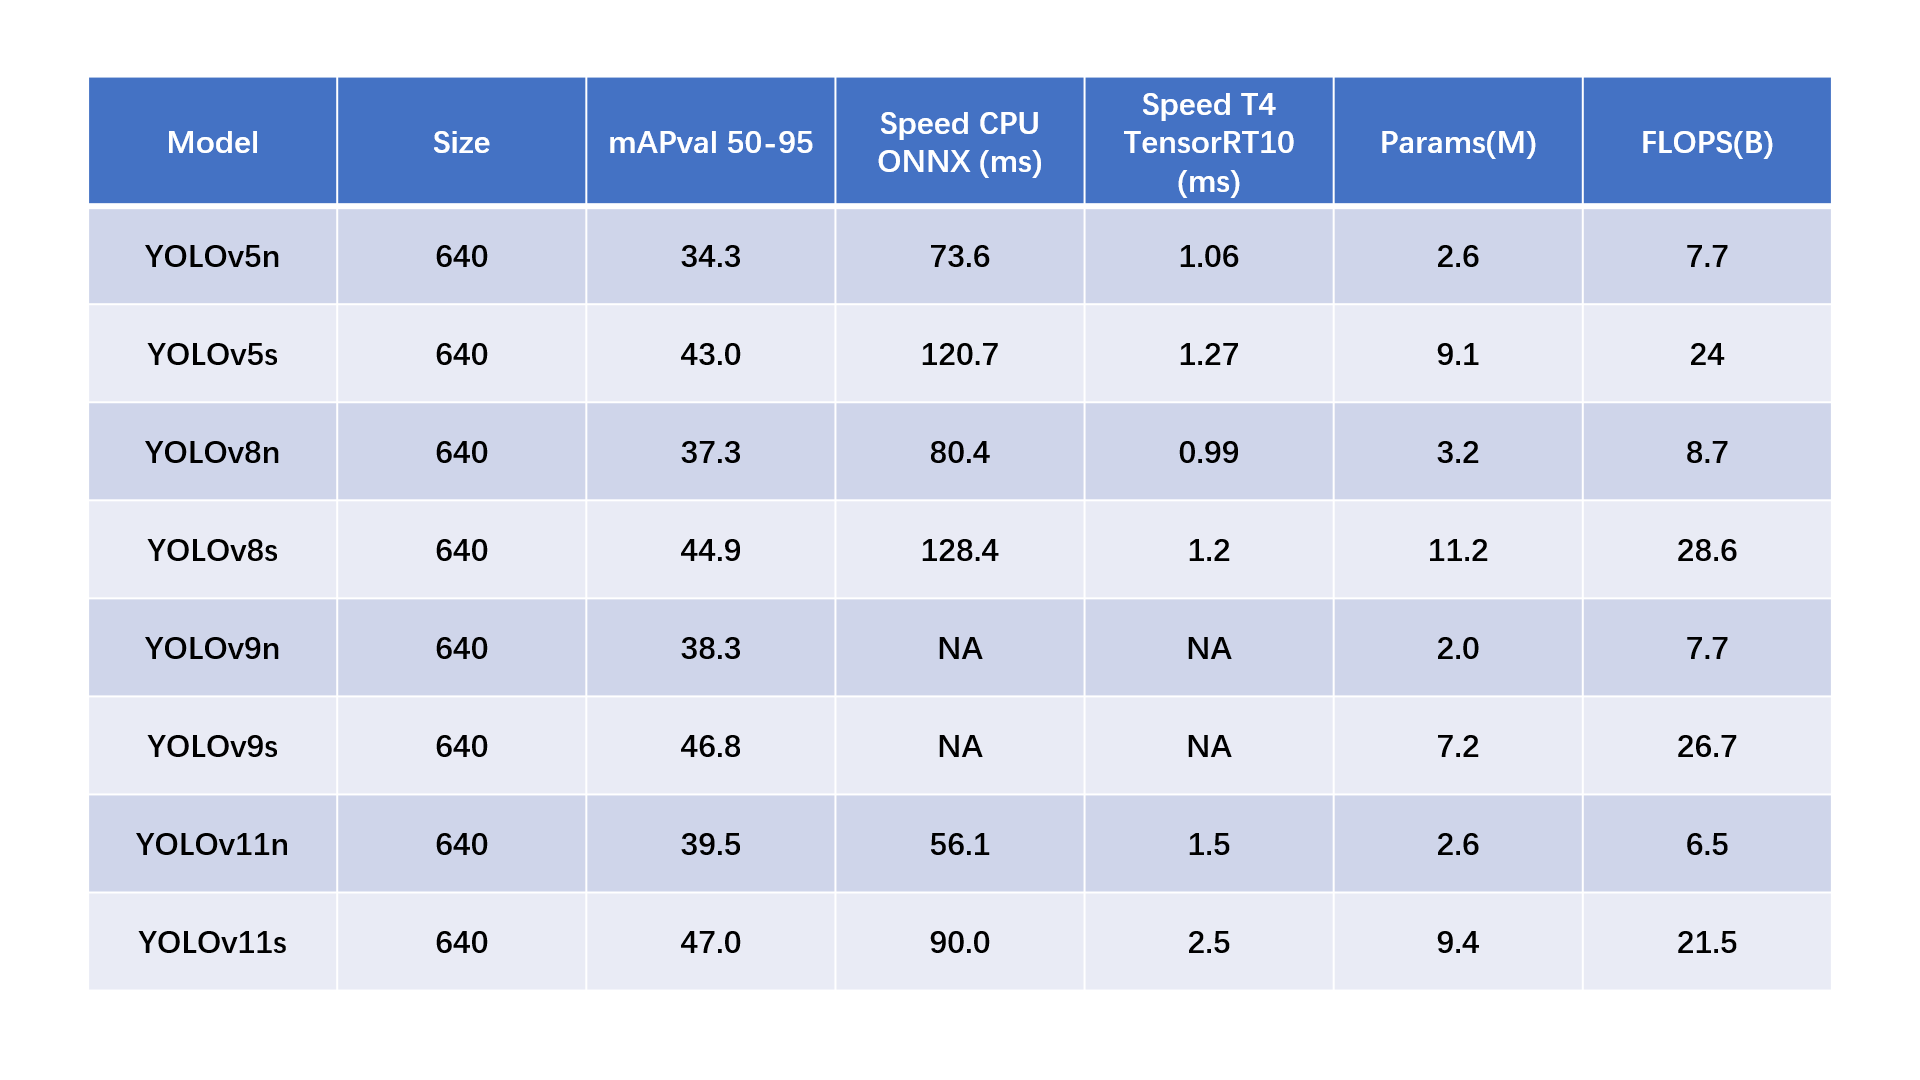
\includegraphics[width=0.85\textwidth]{figs/chap02/compare.png}
%   \caption{YOLO各版本模型性能对比}
%   \label{fig:compare}
% \end{figure}

\section{数据集预处理}
本文所使用的数据集来源于缅甸真实的交通道路照片,该数据集为公开资源(数据集来源:\url{https://www.cvmart.net/dataSets/detail/627})。首先使用LabelImg工具对数据集进行标注,生成xml格式的标注文件,再转换成YOLO格式的txt标注文件。YOLO所使用的txt标注文件的格式如\ref{tab:format}所示,文件的每一行有五个元素,其中中心点位置由x\_center和y\_center两个参数描述,分别对应于图像宽度和高度的相对比例值;而边界框的尺寸特征则通过width和height两个参数表征,同样表示为相对于图像原始宽度和高度的归一化比例值。上述五元组能够表示某一个类别的目标在图像中的位置。

\begin{table}[htb]
      \centering
      \caption[目标数据]{YOLO数据标注格式\label{tab:format}}
      \begin{tabular}{lrrrr}
          \toprule
          \multicolumn{1}{c}{class} & \multicolumn{1}{c}{x\_center} & \multicolumn{1}{c}{y\_center} & \multicolumn{1}{c}{width} & \multicolumn{1}{c}{height} \\
          \midrule
          5 & 0.18229123 & 0.72314815 & 0.09270814 & 0.19629641 \\
          14 & 0.40755224 & 0.68564817 & 0.05677574 & 0.18796234 \\
          15 & 0.84505233 & 0.61064834 & 0.04947934 & 0.12587944 \\
          \bottomrule
      \end{tabular}
\end{table}


本文的原数据集包含5661张摩托车驾乘人员头盔佩戴情况图像,由于其中某些类别的样本数据非常少,对包含这些标签的原图像进行了图像增强,保证每一个类别至少有100张样本图像。具体的增强方法如\ref{fig:enhance}所示。

\begin{figure}[htbp]
    \centering
    \begin{subfigure}[t]{0.3\textwidth}
        \centering
        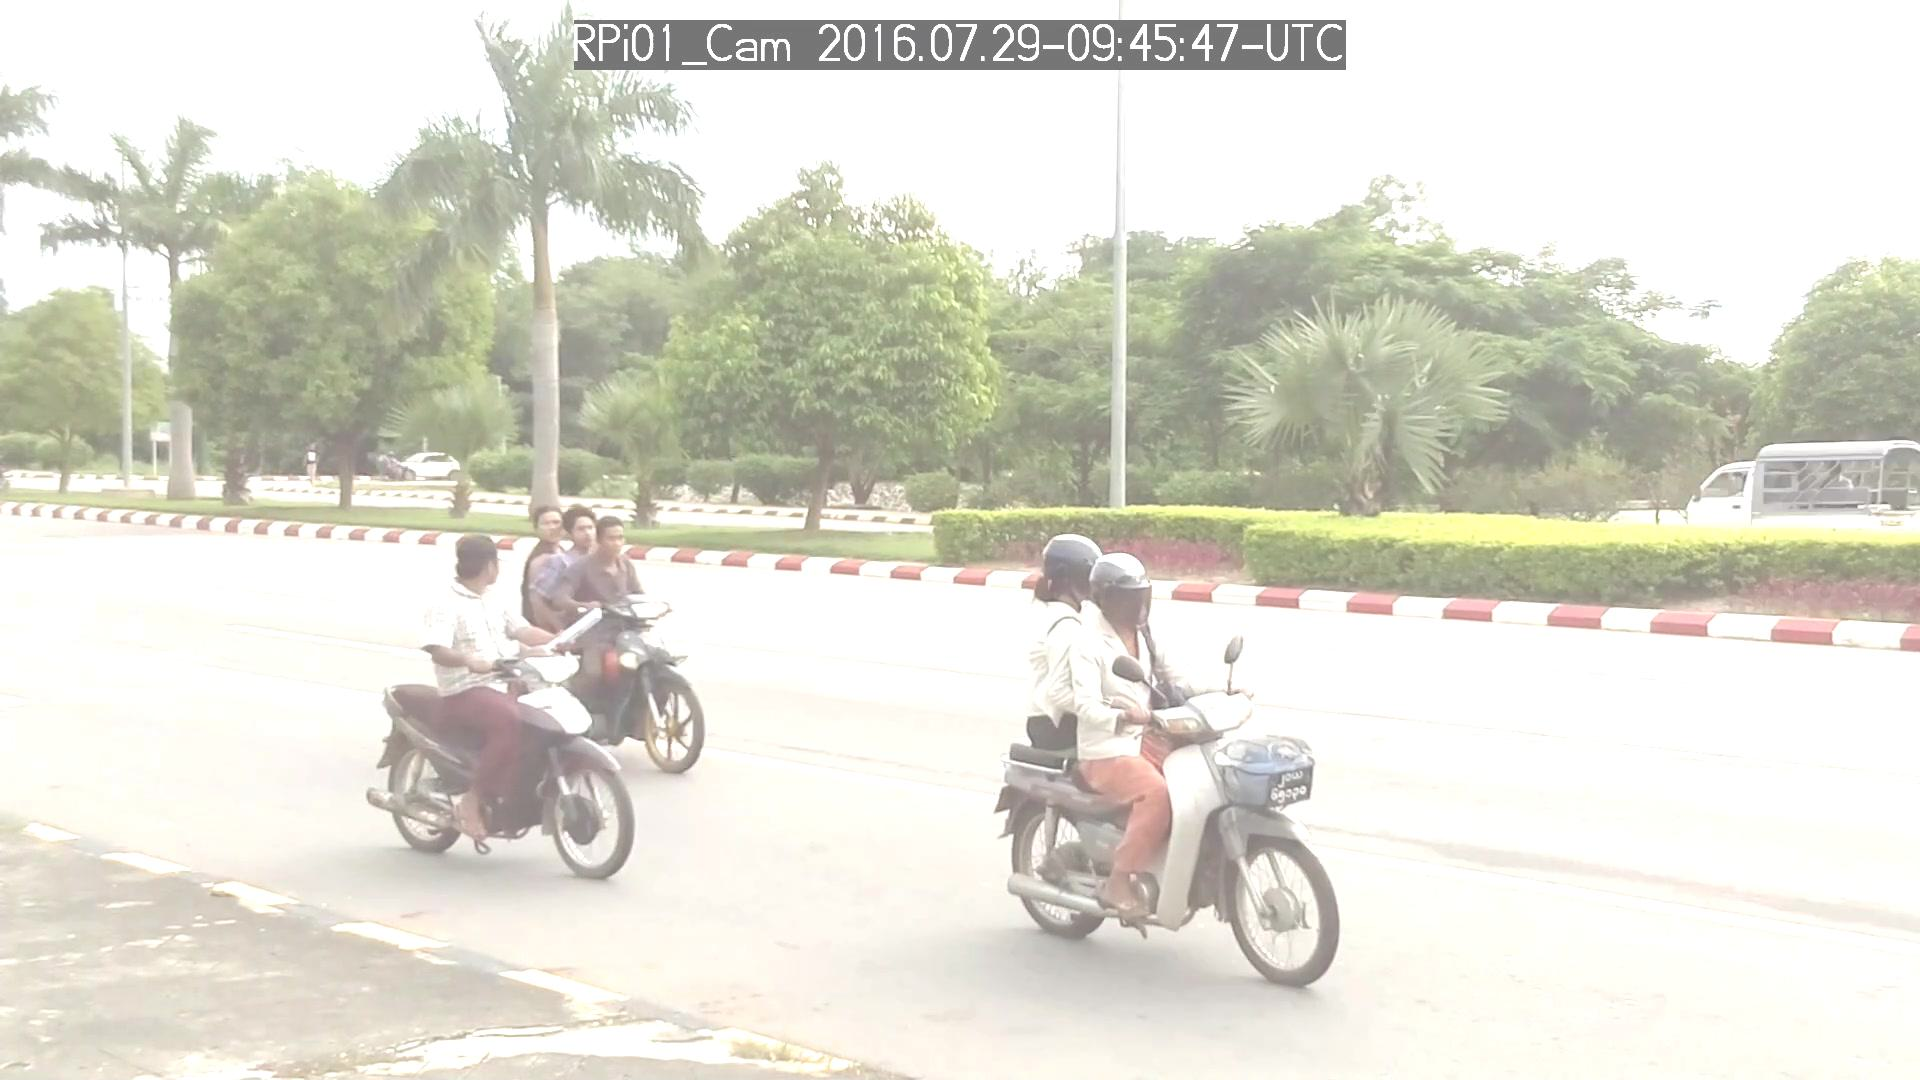
\includegraphics[width=\textwidth]{figs/chap03/rb_origin.jpg}
        \caption{随机亮度}
        \label{fig:sub1}
    \end{subfigure}
    \begin{subfigure}[t]{0.3\textwidth}
        \centering
        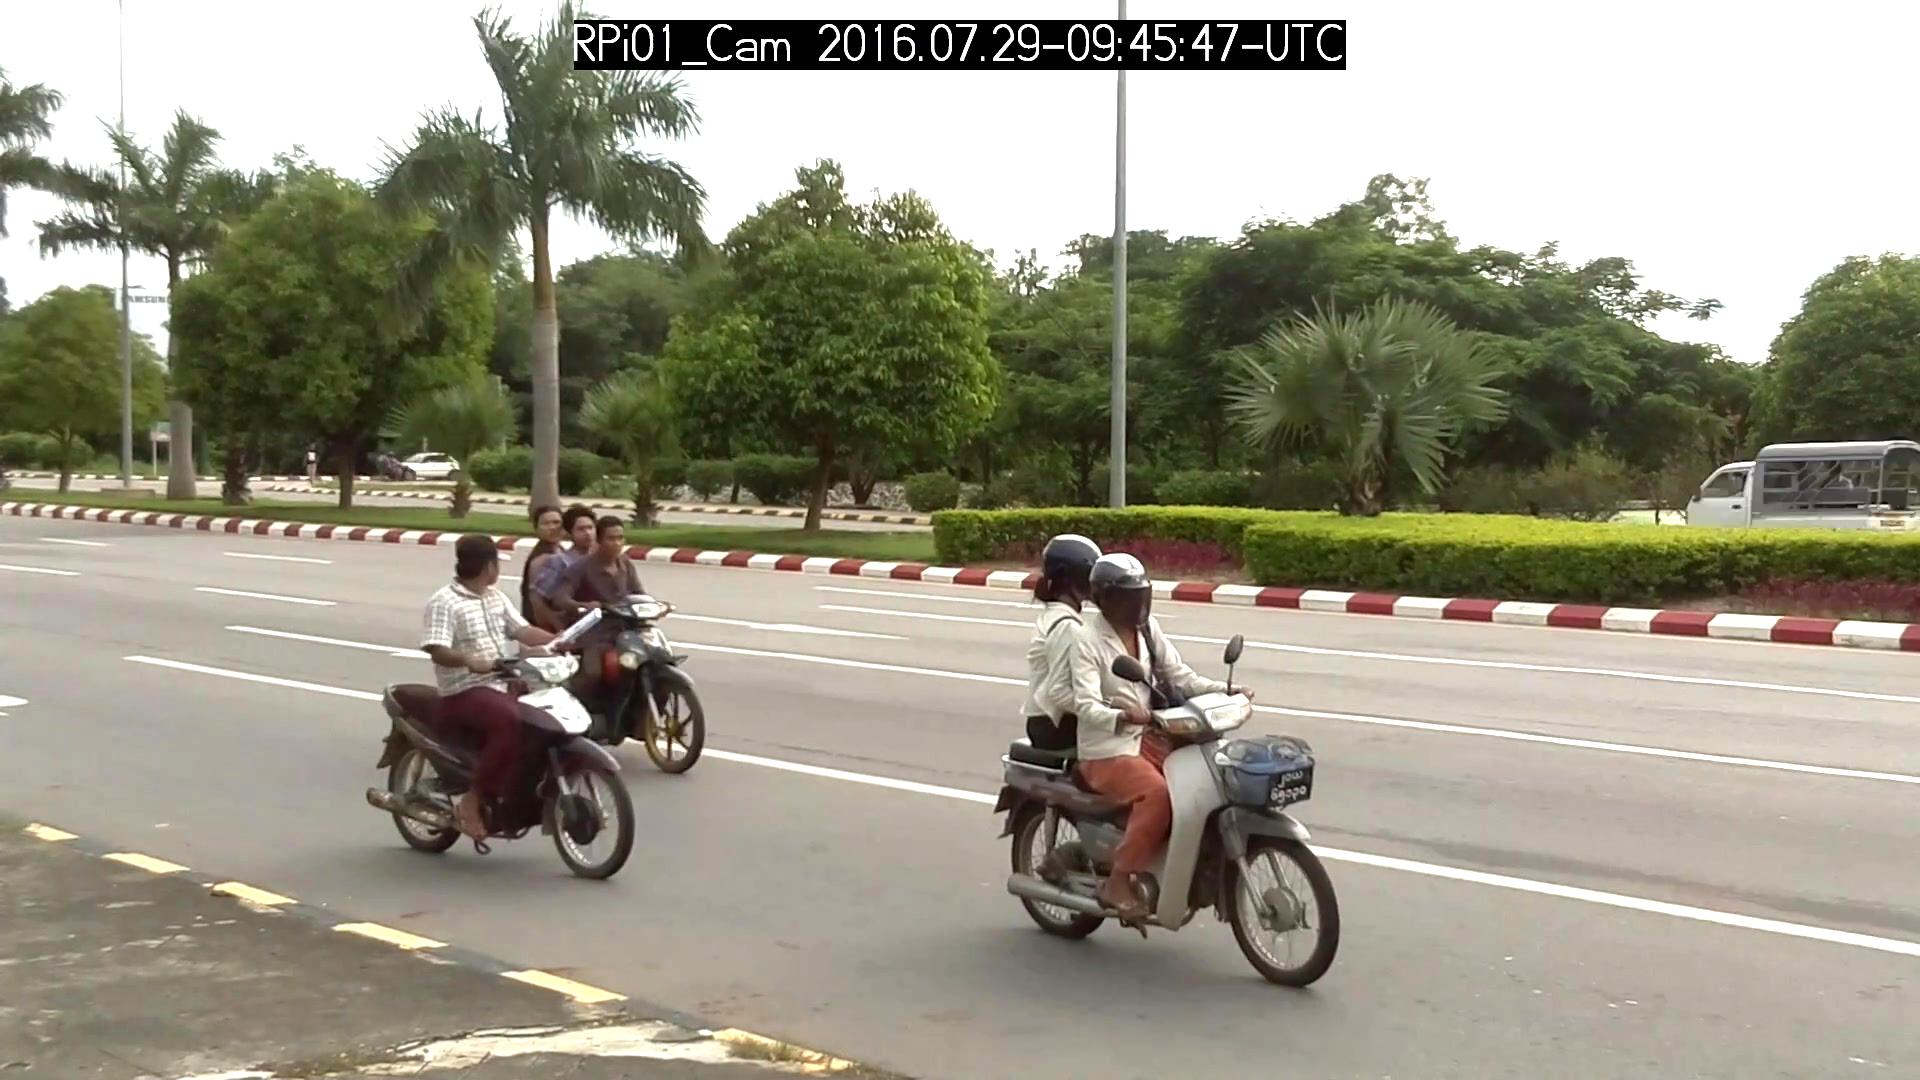
\includegraphics[width=\textwidth]{figs/chap03/rc_origin.jpg}
        \caption{随机对比度}
        \label{fig:sub2}
    \end{subfigure}
    \begin{subfigure}[t]{0.3\textwidth}
        \centering
        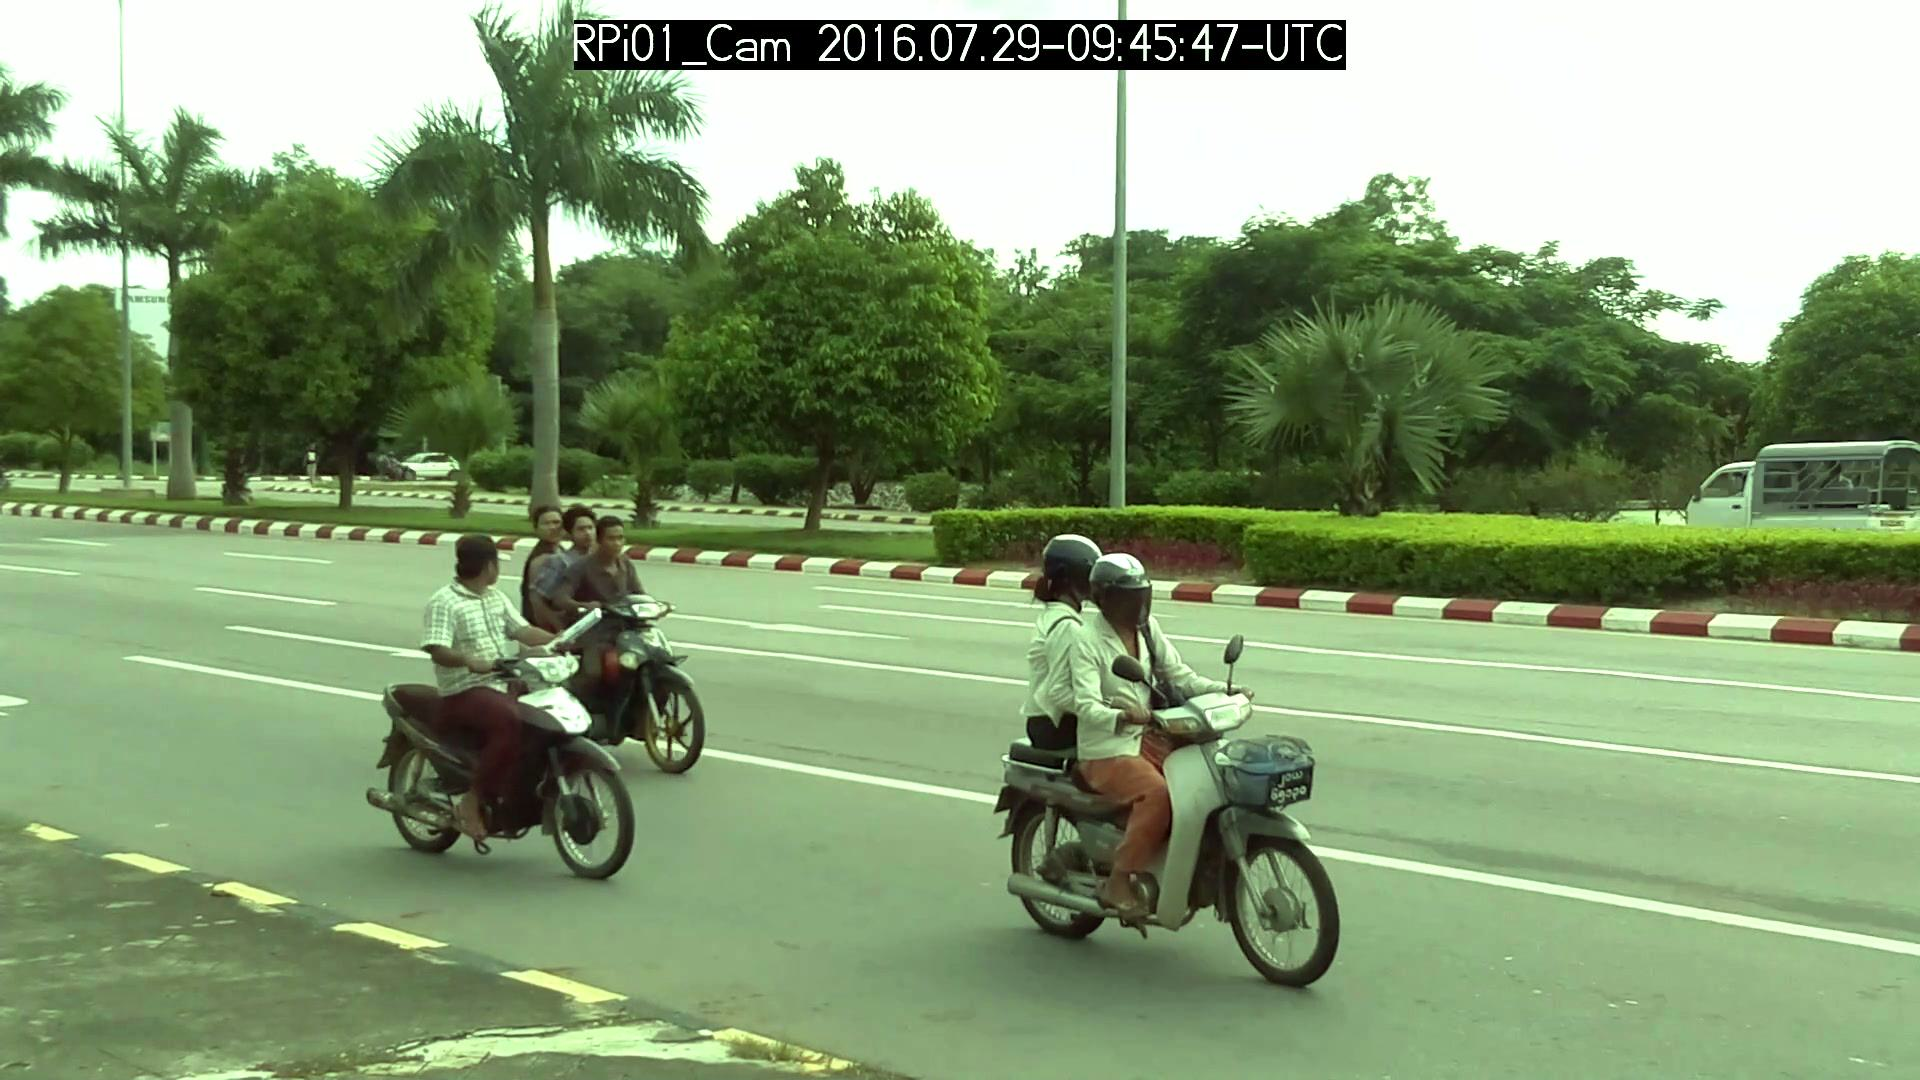
\includegraphics[width=\textwidth]{figs/chap03/rs_origin.jpg}
        \caption{随机饱和度}
        \label{fig:sub3}
    \end{subfigure}

    \begin{subfigure}[t]{0.3\textwidth}
        \centering
        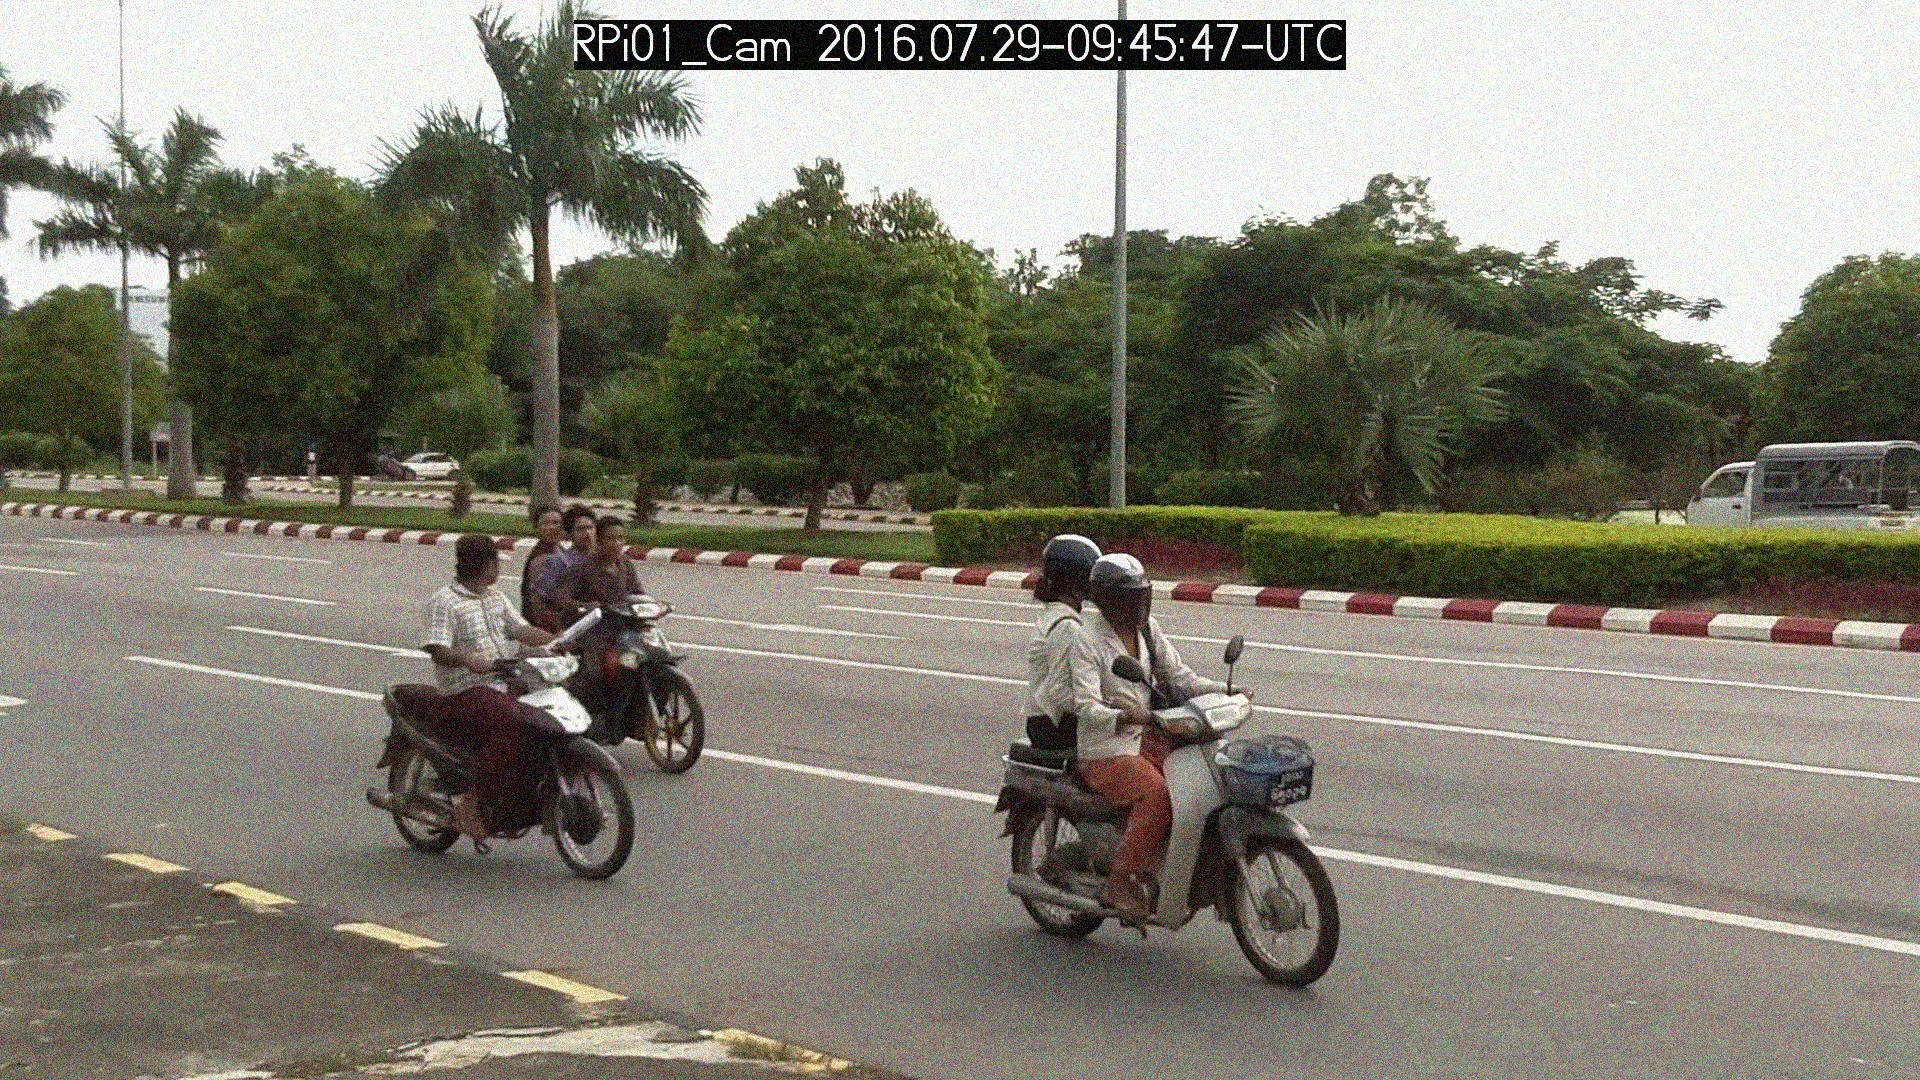
\includegraphics[width=\textwidth]{figs/chap03/gn_origin.jpg}
        \caption{高斯噪声}
        \label{fig:sub4}
    \end{subfigure}
    \begin{subfigure}[t]{0.3\textwidth}
        \centering
        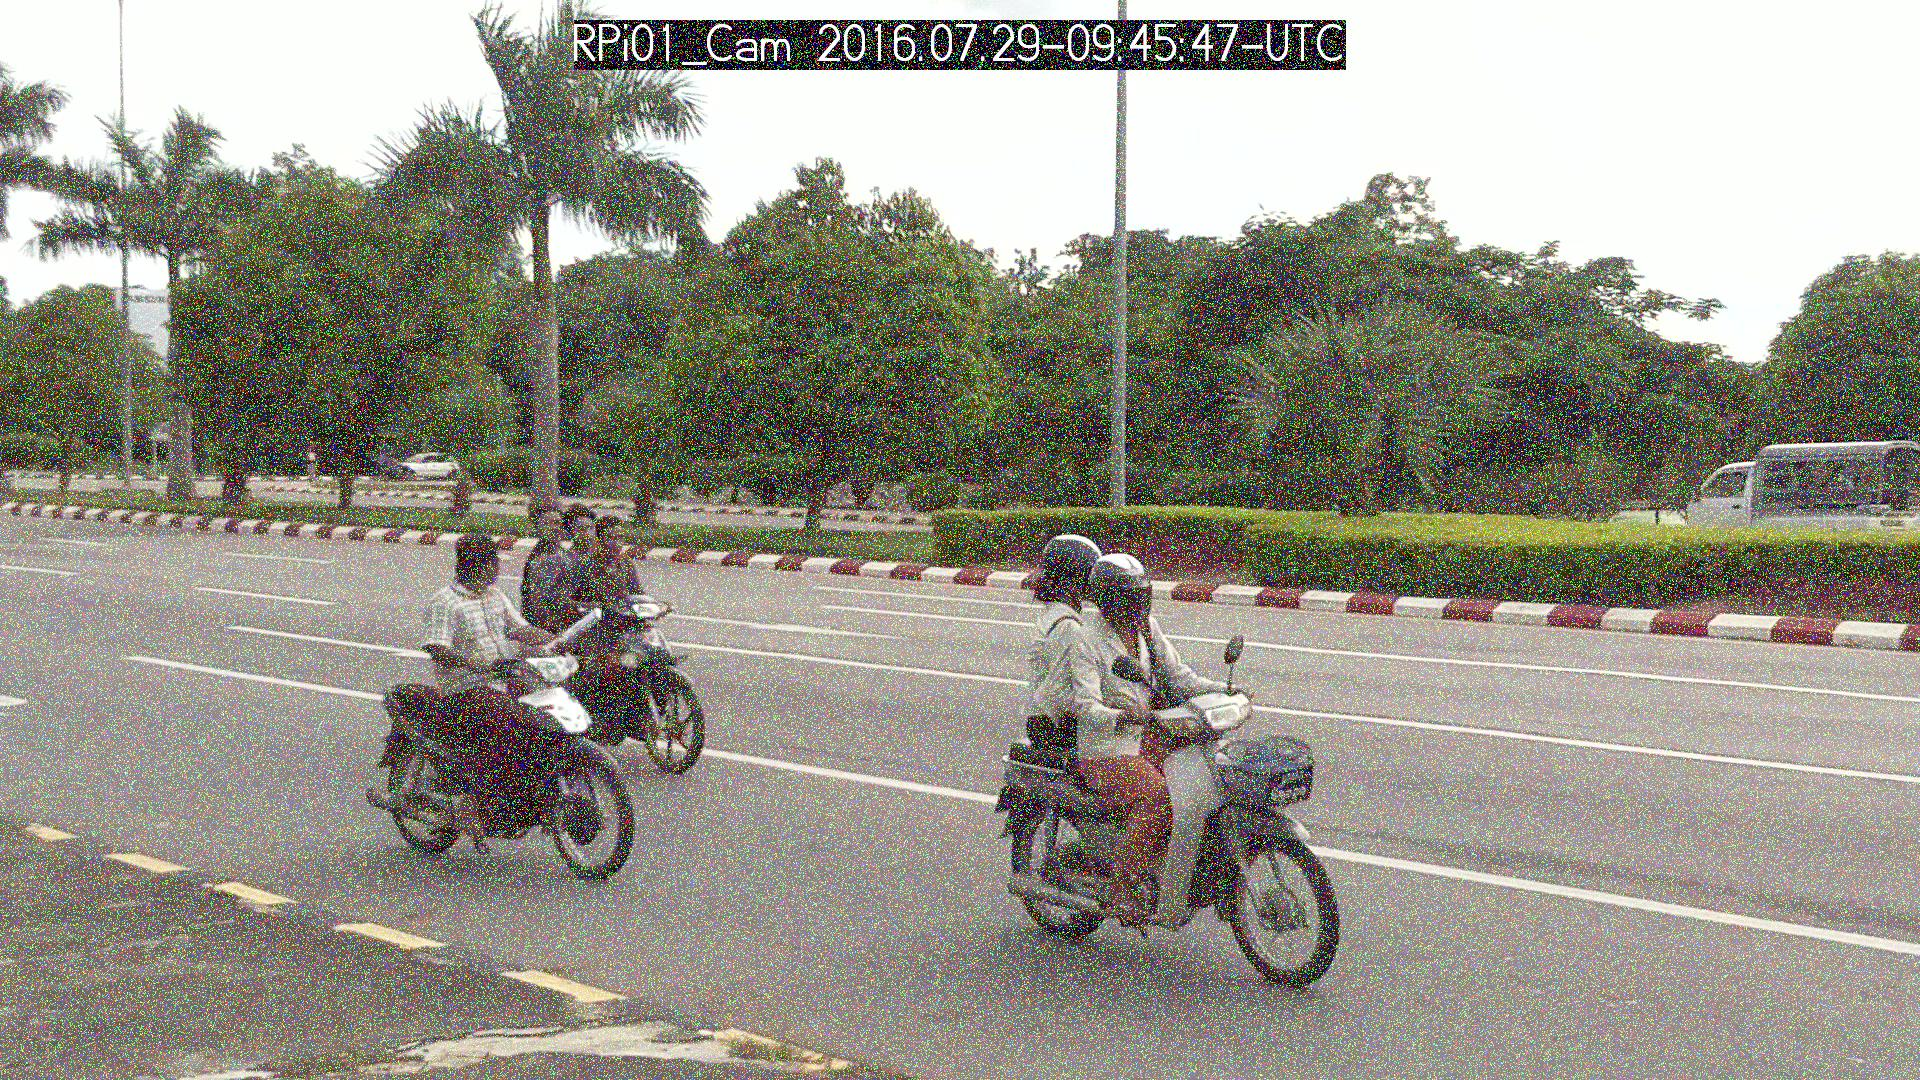
\includegraphics[width=\textwidth]{figs/chap03/sn_origin.jpg}
        \caption{salt噪声}
        \label{fig:sub5}
    \end{subfigure}
    \begin{subfigure}[t]{0.3\textwidth}
        \centering
        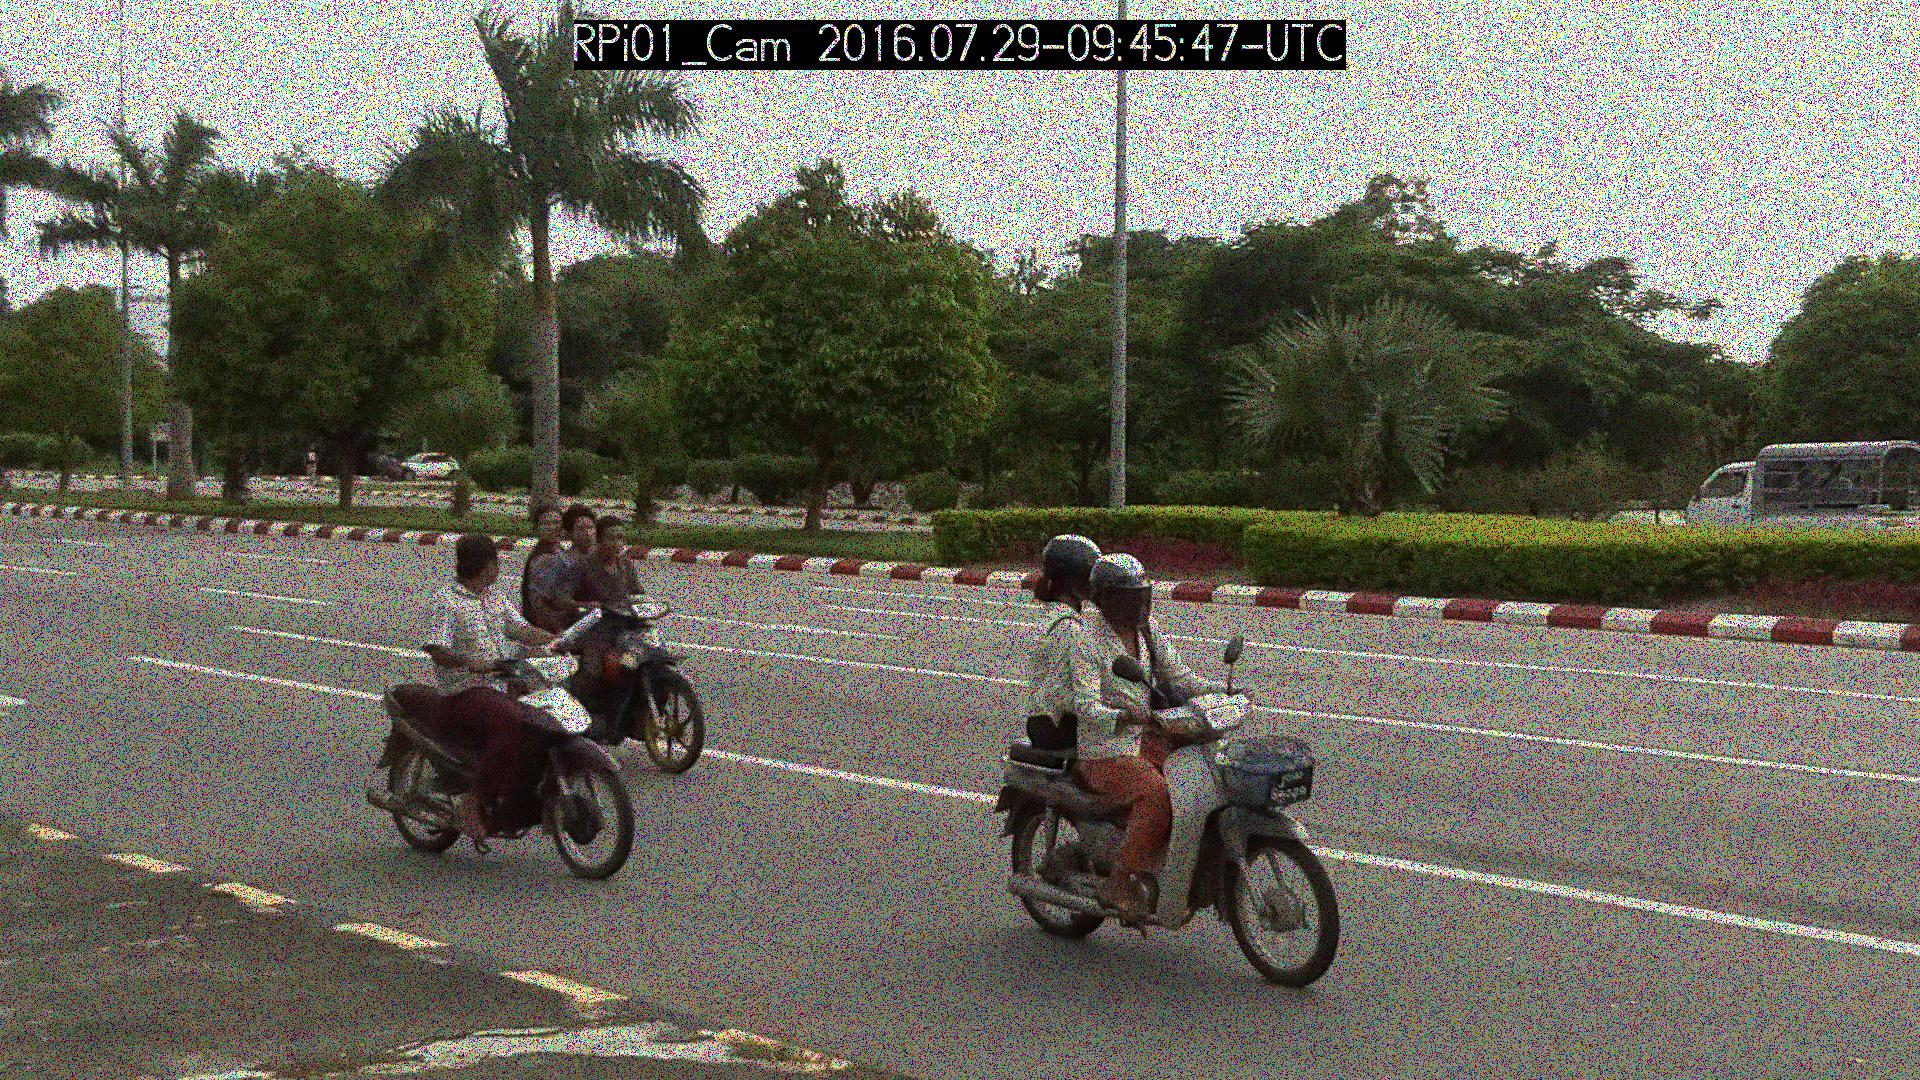
\includegraphics[width=\textwidth]{figs/chap03/pn_origin.jpg}
        \caption{pepper噪声}
        \label{fig:sub6}
    \end{subfigure}
    \caption{图像增强方式}
    \label{fig:enhance}
\end{figure}

对原数据集进行增强之后,共有6282张图像,采用7:2:1的比例对数据集进行随机划分,分别构建训练集、验证集和测试集。本文将目标类别分为18类,标签为S01-S18,其对应关系以及含义如\ref{tab:newlabel}所示,其中meaning一列命名规则为:D(Driver)代表摩托车驾驶员,P(Partner)代表乘车人员。P1代表驾驶员身后的一名乘车人员,P2代表驾驶员身后的另一名乘车人员,P0代表驾驶员身前的乘车人员(在原数据集中,某些小朋友会坐在驾驶员身前)。而D、P0、P1和P2后面紧跟着该乘车人员的头盔佩戴情况,Helmet代表已佩戴头盔,NoHelmet代表未佩戴头盔。例如,标签为S09的含义为DNoHelmetP0NoHelmetP1NoHelmet,表示摩托车驾驶员D未佩戴头盔,驾驶员身前的乘车人员P0未佩戴头盔,驾驶员身后的一名乘车人员P1未佩戴头盔。

\begin{table}[htb]
    \centering
    \caption[标签解释]{目标类别标签含义\label{tab:newlabel}}
    \begin{tabular}{lcl}
        \toprule
        \multicolumn{1}{c}{class} & \multicolumn{1}{c}{label} & \multicolumn{1}{l}{meaning} \\
        \midrule
        0 & S01 & DHelmetP1NoHelmetP2NoHelmet \\
        1 & S02 & DNoHelmetP1NoHelmetP2NoHelmet \\
        2 & S03 & DHelmetP0NoHelmetP1NoHelmet \\
        3 & S04 & DNoHelmetP1NoHelmet \\
        4 & S05 & DHelmetP0NoHelmet \\
        5 & S06 & DNoHelmet \\
        6 & S07 & DNoHelmetP1NoHelmetP2Helmet \\
        7 & S08 & DHelmetP1NoHelmet \\
        8 & S09 & DNoHelmetP0NoHelmetP1NoHelmet \\
        9 & S10 & DNoHelmetP1Helmet \\
        10 & S11 &  DHelmetP0NoHelmetP1Helmet \\
        11 & S12 &  DNoHelmetP0NoHelmetP1NoHelmetP2NoHelmet \\
        12 & S13 &  DHelmetP1NoHelmetP2Helmet \\
        13 & S14 &  DNoHelmetP0NoHelmet \\
        14 & S15 &  DHelmet \\
        15 & S16 &  DHelmetP1Helmet \\
        16 & S17 &  DHelmetP0Helmet \\
        17 & S18 &  DHelmetP1HelmetP2Helmet \\
        \bottomrule
    \end{tabular}
\end{table}

18个类别的样本数量分布如\ref{fig:label1}所示,可以看出S15标签数量最多,共6742个,其表示单一驾驶员佩戴头盔;S06标签数量次之,共6346个,其表示单一驾驶员未佩戴头盔,二者实例数量远高于其他标签。说明单一驾驶员驾驶摩托车是最常出现的情况,且佩戴头盔要比不佩戴头盔的情况稍多一些。除上述两个标签之外,S16和S04是数量最多的两个标签,S16标签共3296个,表示驾驶员和身后的一名乘客都佩戴头盔;S04标签共2503个,表示驾驶员和身后的一名乘客都未佩戴头盔。

由表中数据可以看出,单一驾驶员驾驶摩托车的情况出现次数最多,其次是驾驶员携带一名乘客的情况。并且不管是单一驾驶员,还是驾驶员携带一名乘客,佩戴头盔的情况均多于不佩戴头盔的情况。而一名驾驶员携带一名以上乘客的情况比较少见。

\begin{figure}[!htb]
    \centering
    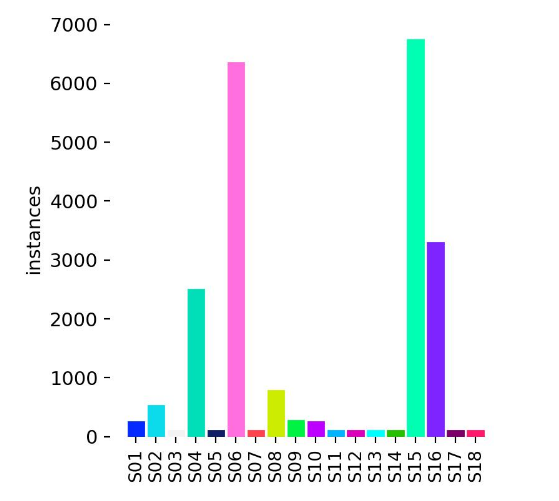
\includegraphics[width=0.8\textwidth]{figs/chap03/label1.png}
    \caption{头盔佩戴情况标签数量分布}
    \label{fig:label1}
\end{figure}

对原数据集5661张图像中的每一个驾驶员目标框进行裁剪,得到33571张包含驾驶员信息的图像,共有570个不同驾驶员。由于驾驶员的图像样本也存在不平衡的情况,对这33571张图像同样进行图像增强,保证每一个驾驶员都至少有100张样本图像。

% \begin{figure}[!htb]
%       \centering
%       \begin{minipage}{0.45\textwidth} % 调整宽度以适应需求,两张图总宽度接近1
%           \centering
%           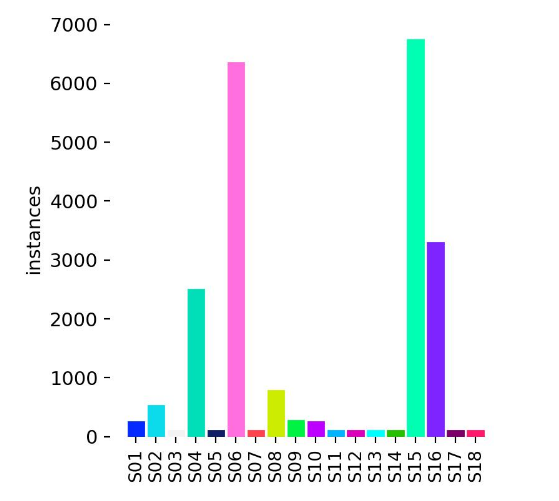
\includegraphics[width=\textwidth]{figs/chap03/label1.png}
%           \caption{头盔佩戴情况标签数量分布}
%           \label{fig:label1}
%       \end{minipage}
%       \hfill % 使两张图像之间保持一定距离
%       \begin{minipage}{0.45\textwidth}
%           \centering
%           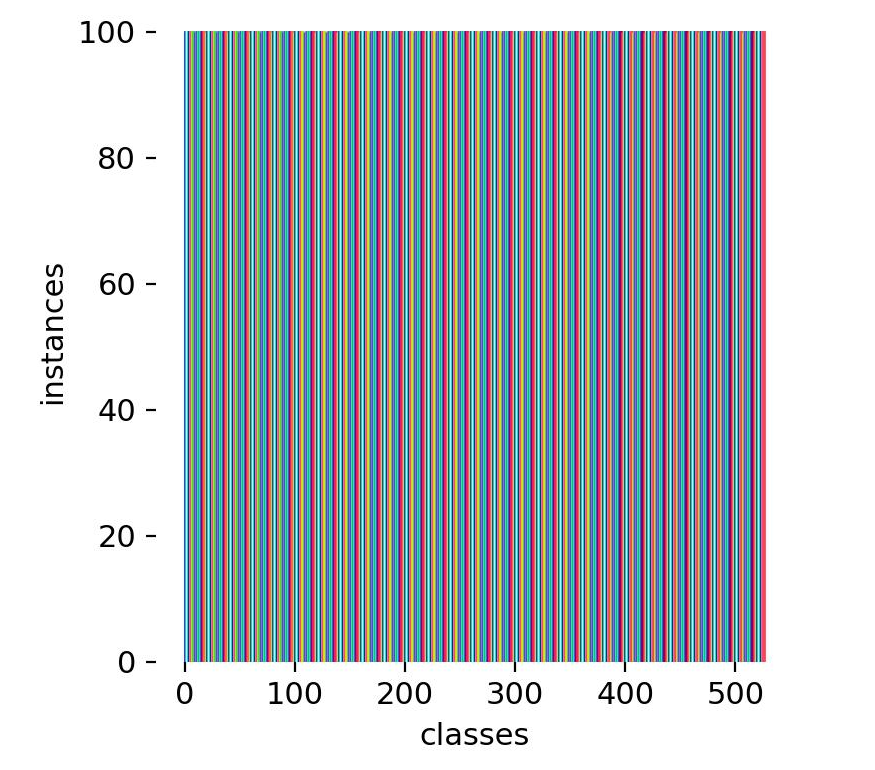
\includegraphics[width=\textwidth]{figs/chap03/label2.png}
%           \caption{驾驶员标签数量分布}
%           \label{fig:label2}
%       \end{minipage}
% \end{figure}

\section{实验环境}
操作系统:Ubuntu 20.04.3 LTS (Focal Fossa)

CPU:Intel(R) Xeon(R) Gold 5318Y CPU @ 2.10GHz

内存:1.5T

GPU:NVIDIA A40

显存:48G

CUDA版本:12.2

Pytorch版本:2.7.0+cu126

\section{参数设置}
本文分别使用YOLOv11n.pt、YOLOv11s.pt、YOLOv11m.pt进行训练,参数设置见\ref{tab:param}。本文进行头盔佩戴情况检测模型训练时,共有18个标签,在yaml文件里nc设置为18。在训练模型中,将batch设置为16,输入图像的size默认设置为640x640,epochs设置为300。
degrees设置为20,在指定度数范围内随机旋转图像,提升模型对摄像头拍摄到的不同角度的图像的识别能力。hsv\_v设置为0.6,将图像的亮度修改一部分,模拟不同的光照环境。translate设置为0.2,将图像进行水平和垂直平移,有助于检测部分可见物体。

\begin{table}[H]
    \centering
    \caption[标签解释]{参数设置\label{tab:param}}
    \begin{tabular}{lll}
        \toprule
        \multicolumn{1}{l}{param} & \multicolumn{1}{l}{value} & \multicolumn{1}{l}{meaing}\\
        \midrule
        nc & 18 & 类别数量\\
        batch & 16 & 训练批次\\
        size & 640x640 & 输入图像的尺寸\\
        epochs & 300 & 训练轮数\\
        degrees & 20 & 控制图像随机旋转的度数范围\\
        hsv\_v & 0.6 & 控制图像亮度调整幅度\\
        translate & 0.2 & 控制图像在水平和垂直方向上的平移程度\\
        \bottomrule
    \end{tabular}
\end{table}

\section{本章小结}
本章首先围绕YOLOv11算法相关理论展开,系统阐述了YOLOv11的网络结构,主要介绍了骨干网络、颈部网络和检测头,说明了YOLOv11对上述三个结构的改进点,并对YOLOv11中三个重要的损失函数做了详细的分析。然后介绍了原数据集的来源和本文使用到的六种数据增强方式,展示了需要训练的两个模型的标签及其数量分布。简要介绍了实验环境以及训练的参数设置。
\chapter{数据集构建及训练参数设置}

\section{数据集构建}
本文所使用的数据集来源于缅甸真实的交通道路照片。首先使用LabelImg工具对数据集进行标注,生成xml格式的标注文件,再转换成YOLO格式的txt标注文件。YOLO所使用的txt标注文件的格式如\ref{tab:format}所示,文件的每一行有五个元素,其中中心点位置由x\_center和y\_center两个参数描述,分别对应于图像宽度和高度的相对比例值;而边界框的尺寸特征则通过width和height两个参数表征,同样表示为相对于图像原始宽度和高度的归一化比例值。上述五元组能够表示某一个类别的目标在图像中的位置。

\begin{table}[htb]
      \centering
      \caption[目标数据]{YOLO数据标注格式\label{tab:format}}
      \begin{tabular}{lrrrr}
          \toprule
          \multicolumn{1}{c}{class} & \multicolumn{1}{c}{x\_center} & \multicolumn{1}{c}{y\_center} & \multicolumn{1}{c}{width} & \multicolumn{1}{c}{height} \\
          \midrule
          5 & 0.18229123 & 0.72314815 & 0.09270814 & 0.19629641 \\
          14 & 0.40755224 & 0.68564817 & 0.05677574 & 0.18796234 \\
          15 & 0.84505233 & 0.61064834 & 0.04947934 & 0.12587944 \\
          \bottomrule
      \end{tabular}
\end{table}


本文的原数据集包含5661张摩托车驾乘人员头盔佩戴情况图片,由于其中某些类别的样本数据非常少,对包含这些标签的原图片进行了图像增强,保证每一个类别至少有100张样本图片。具体的增强方法如\ref{fig:enhance}所示。

\begin{figure}[htbp]
    \centering
    \begin{subfigure}[t]{0.3\textwidth}
        \centering
        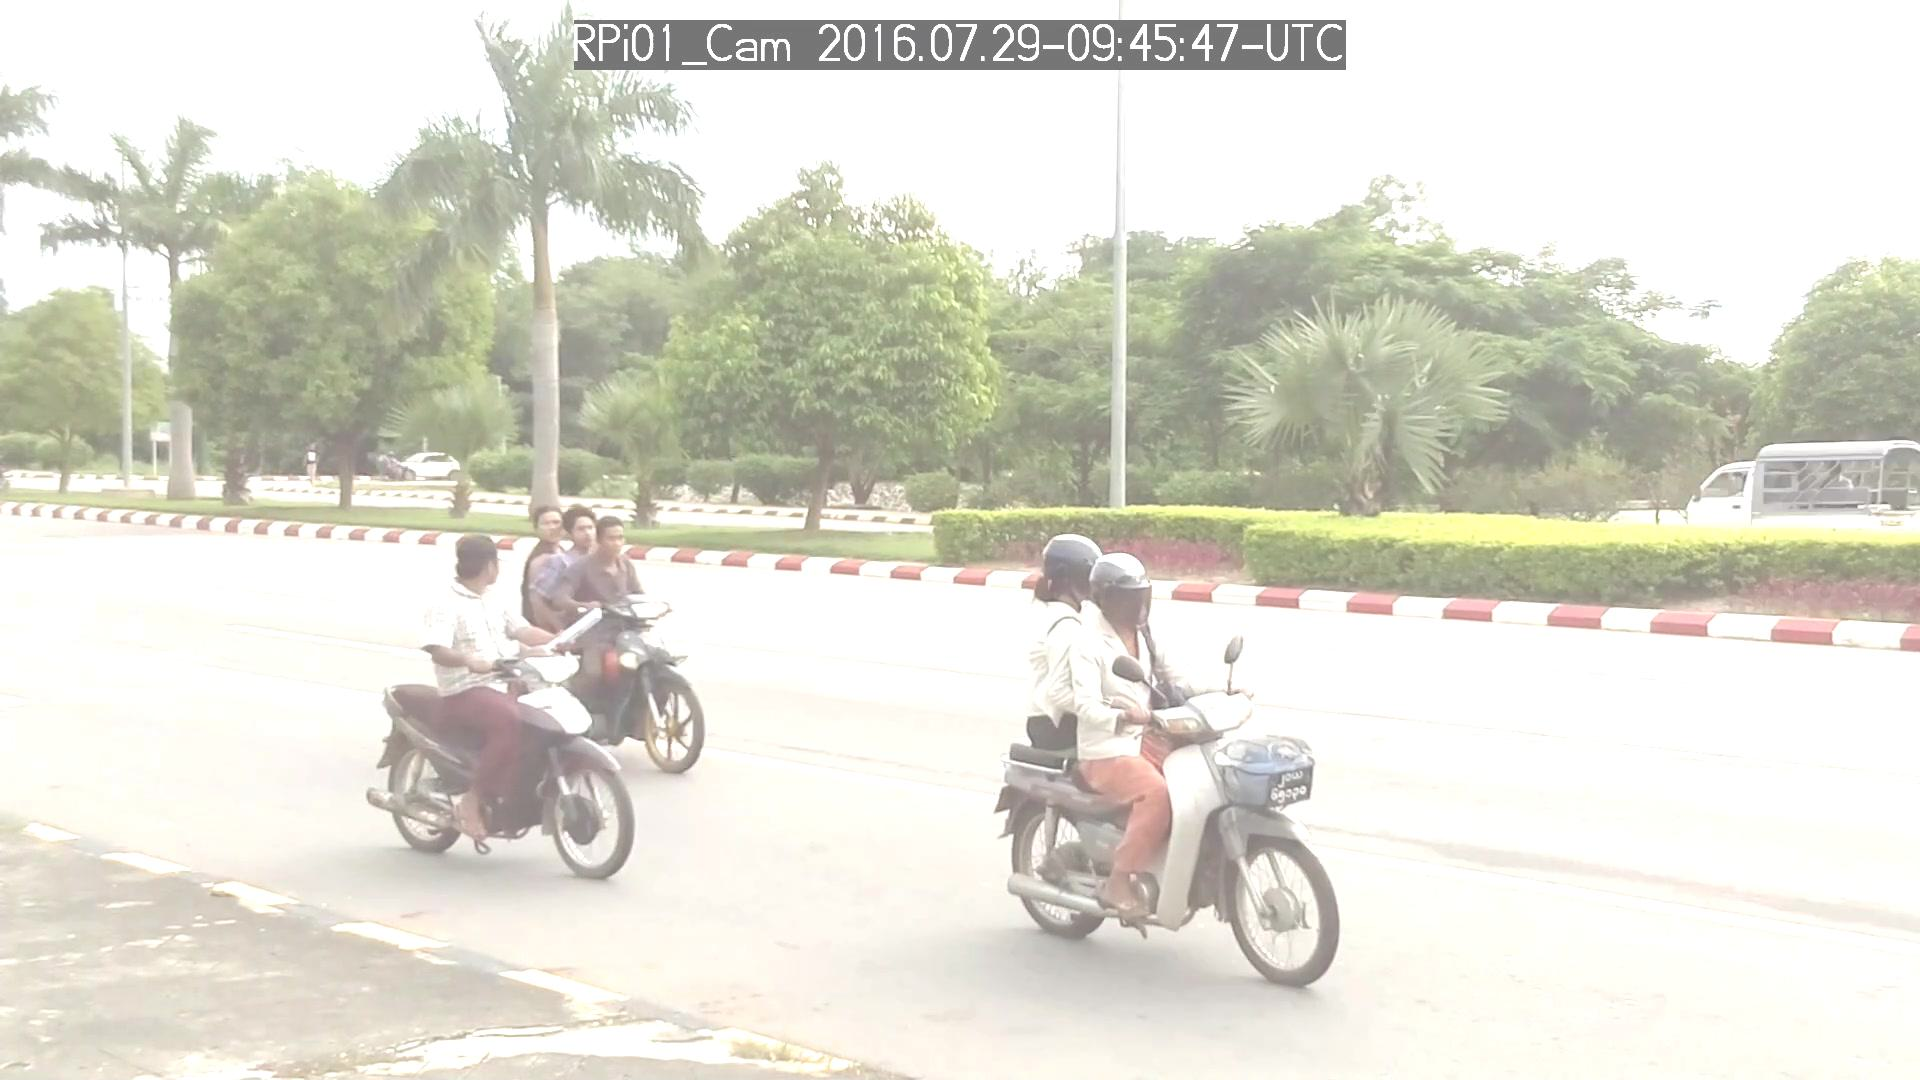
\includegraphics[width=\textwidth]{figs/chap03/rb_origin.jpg}
        \caption{随机亮度}
        \label{fig:sub1}
    \end{subfigure}
    \begin{subfigure}[t]{0.3\textwidth}
        \centering
        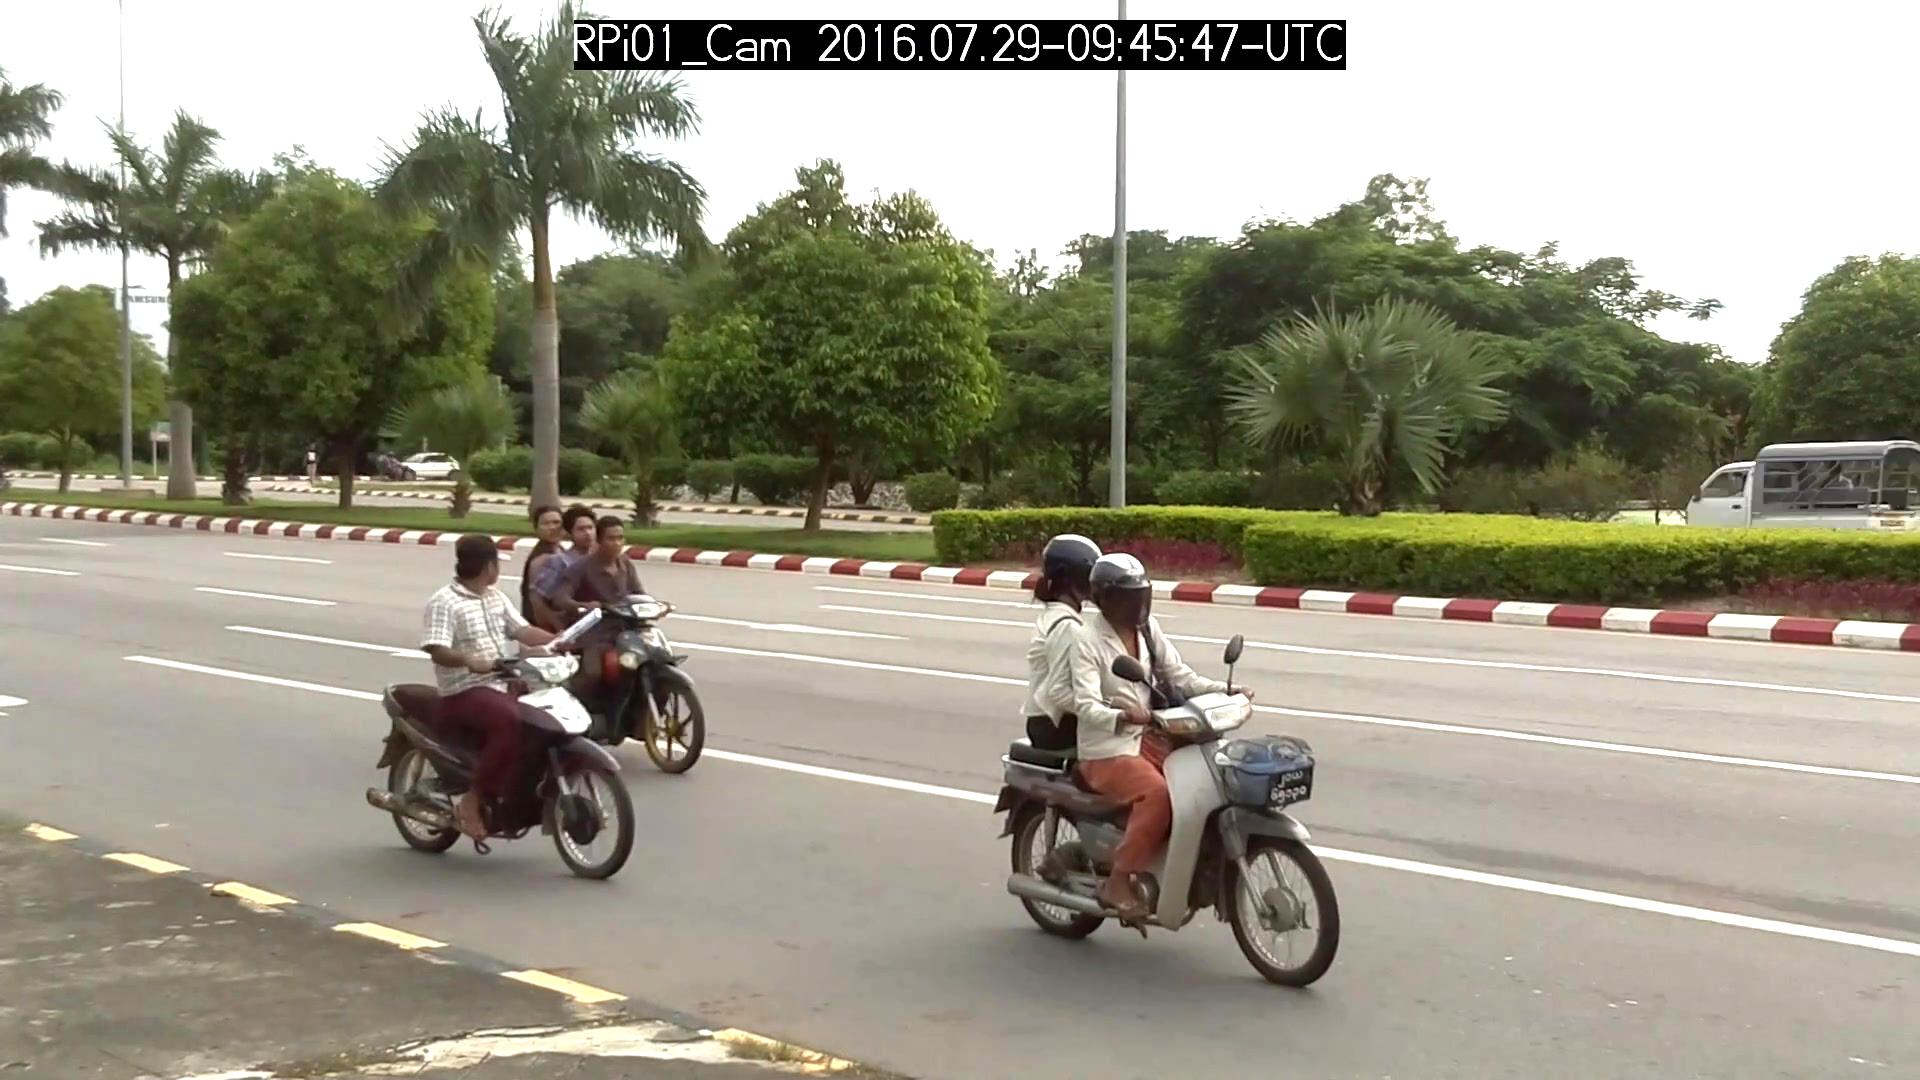
\includegraphics[width=\textwidth]{figs/chap03/rc_origin.jpg}
        \caption{随机对比度}
        \label{fig:sub2}
    \end{subfigure}
    \begin{subfigure}[t]{0.3\textwidth}
        \centering
        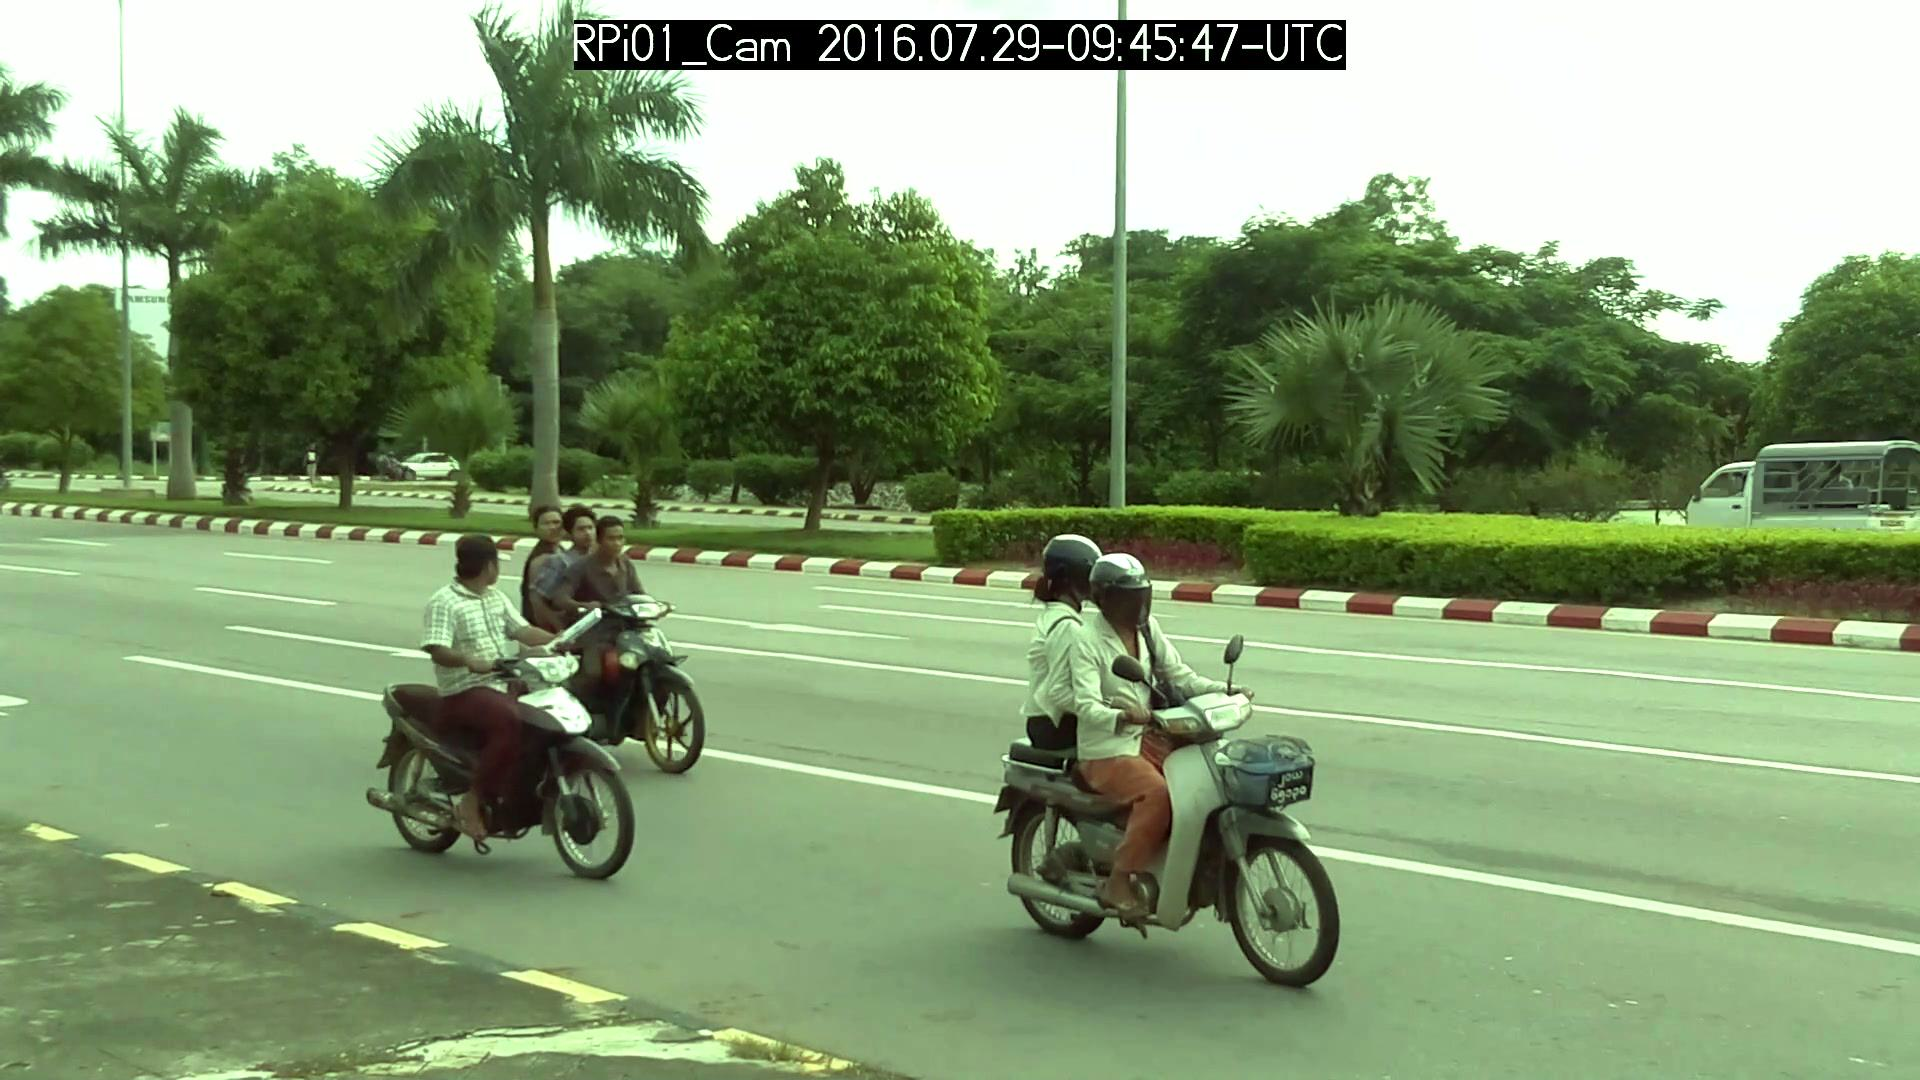
\includegraphics[width=\textwidth]{figs/chap03/rs_origin.jpg}
        \caption{随机饱和度}
        \label{fig:sub3}
    \end{subfigure}

    \begin{subfigure}[t]{0.3\textwidth}
        \centering
        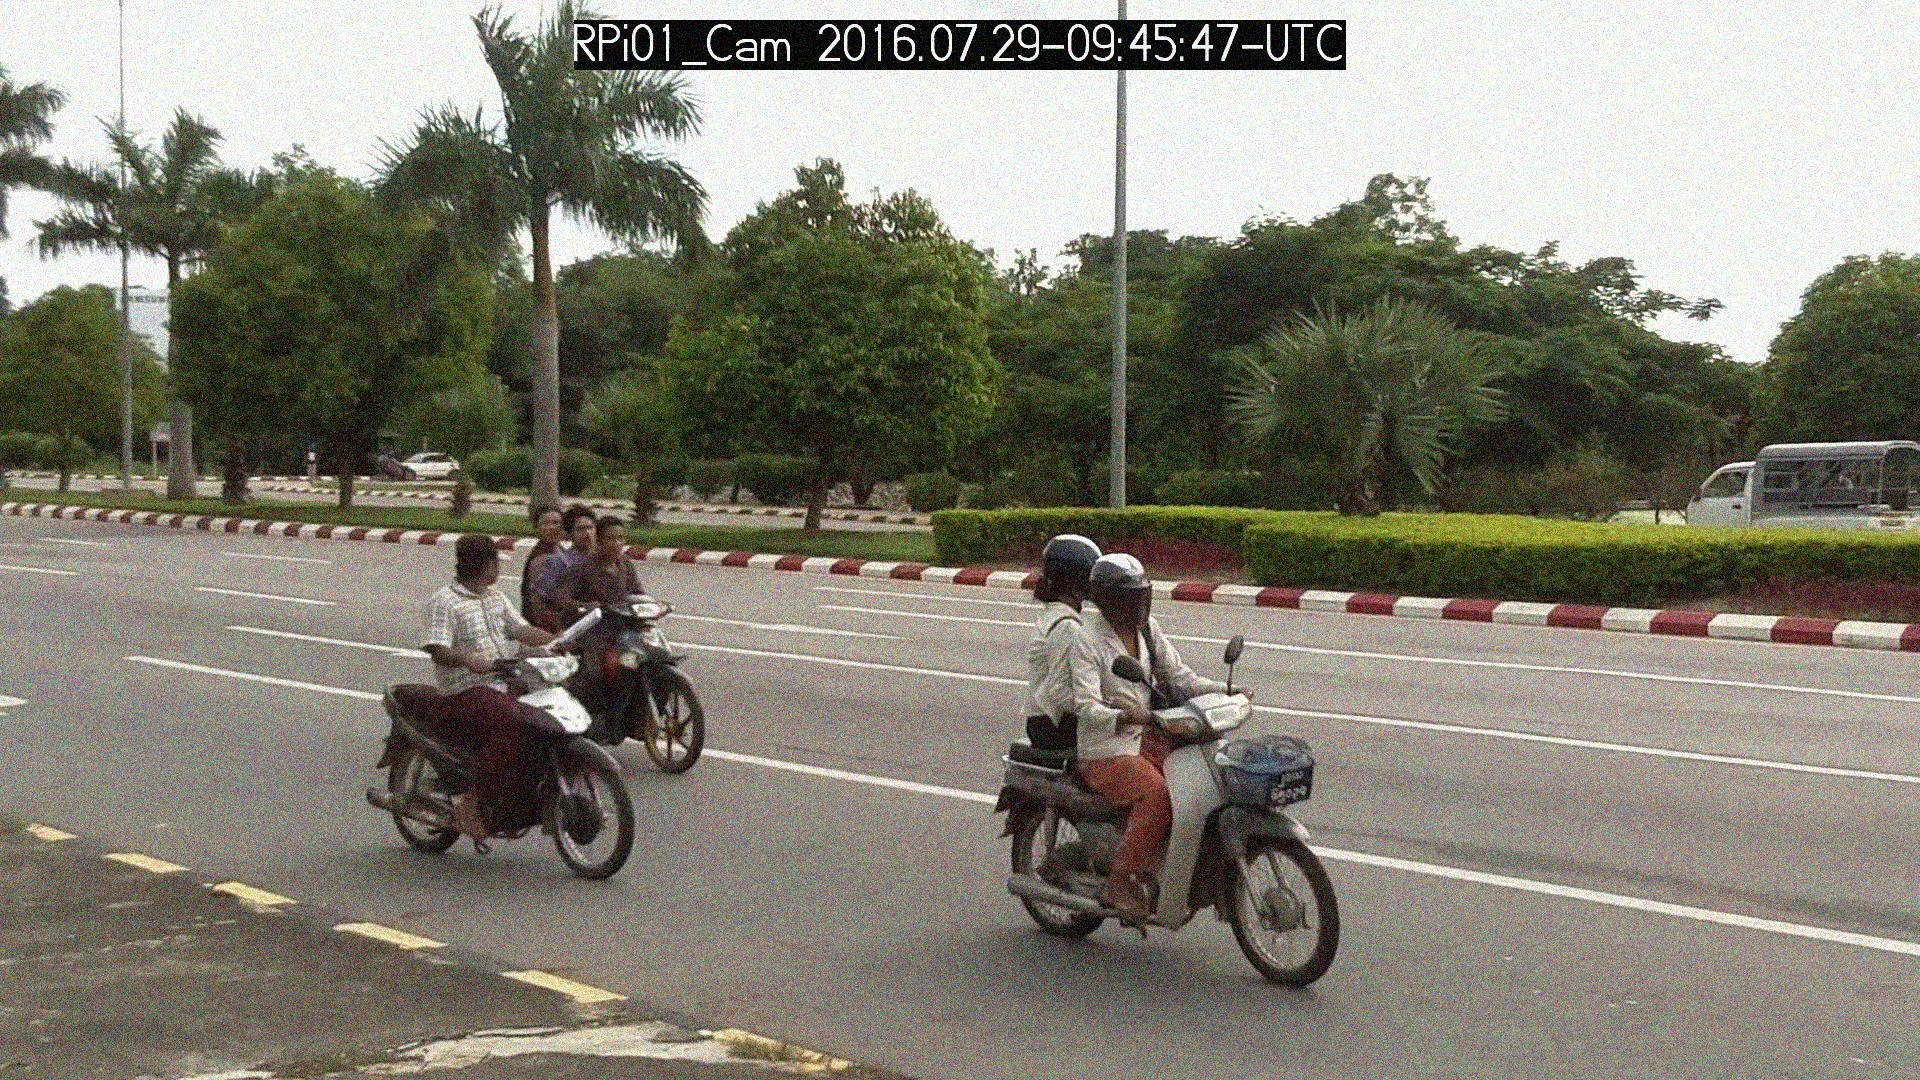
\includegraphics[width=\textwidth]{figs/chap03/gn_origin.jpg}
        \caption{高斯噪声}
        \label{fig:sub4}
    \end{subfigure}
    \begin{subfigure}[t]{0.3\textwidth}
        \centering
        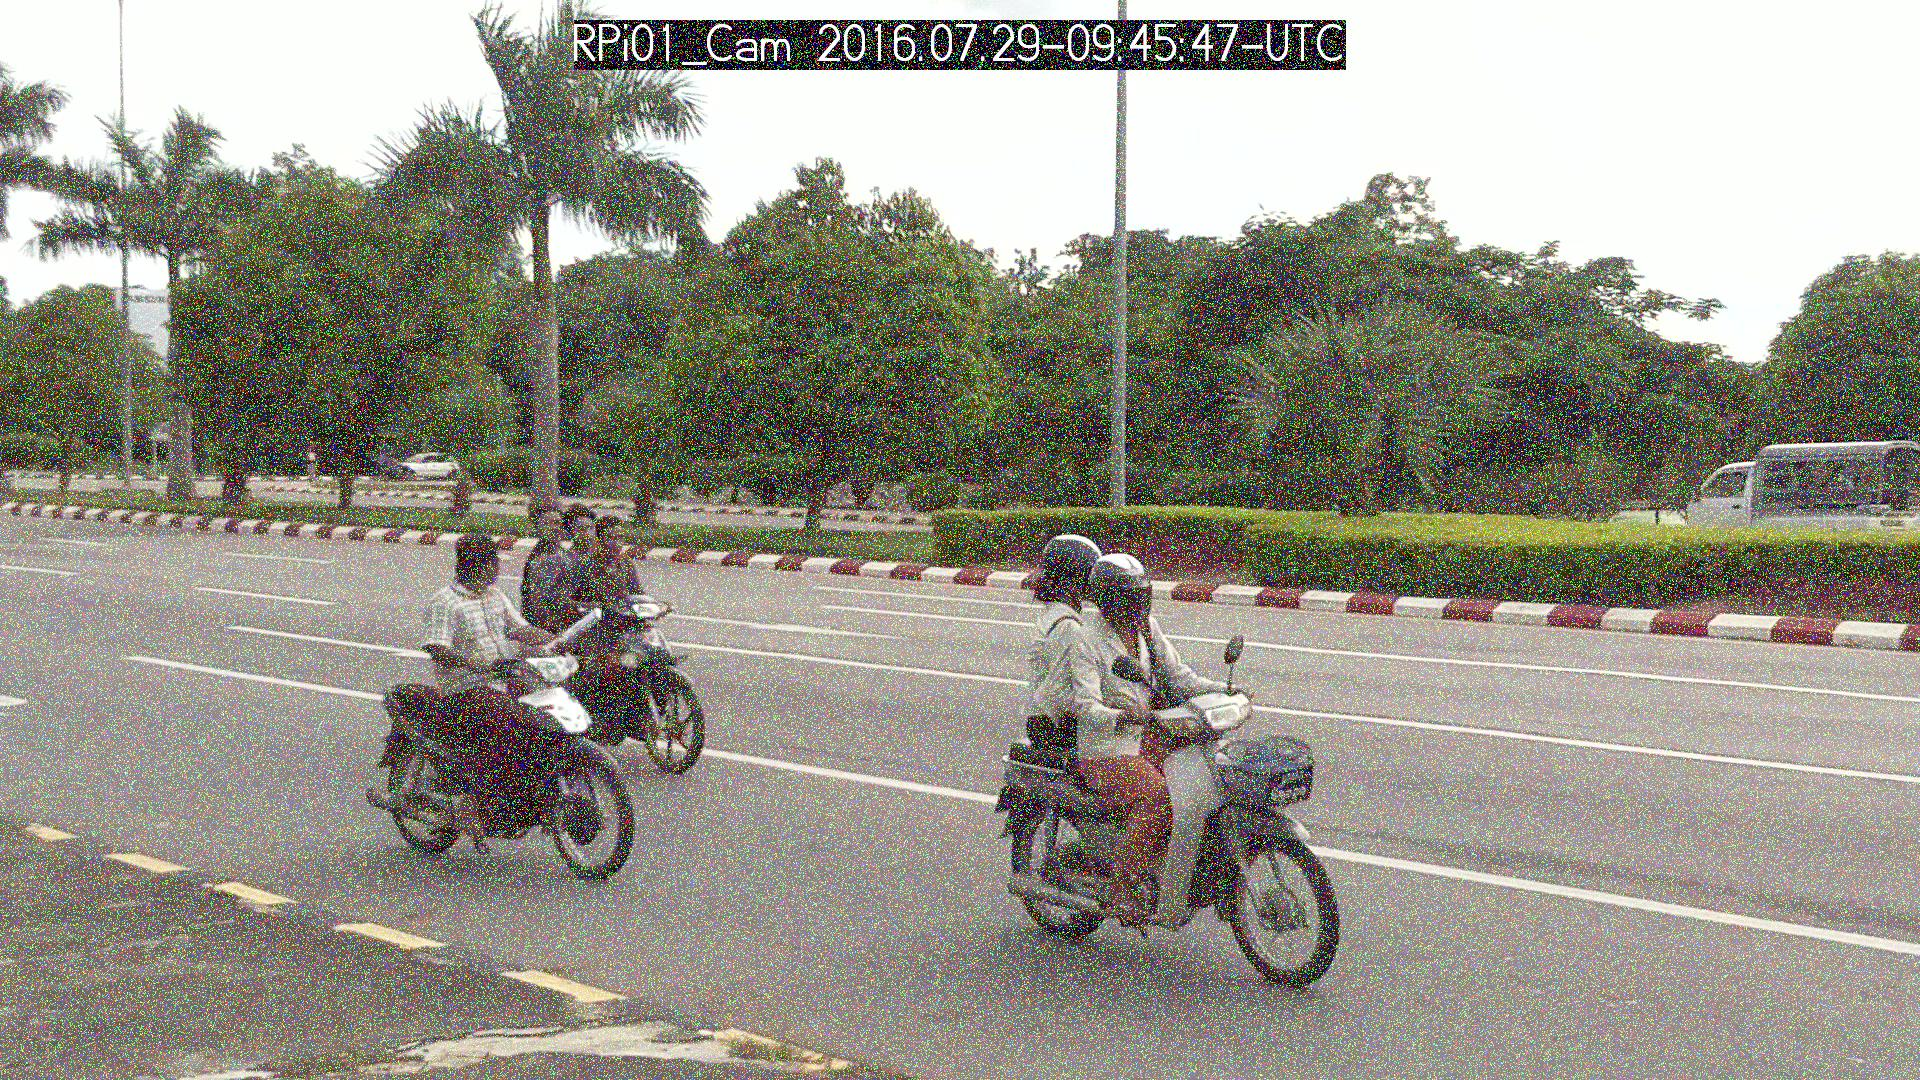
\includegraphics[width=\textwidth]{figs/chap03/sn_origin.jpg}
        \caption{salt噪声}
        \label{fig:sub5}
    \end{subfigure}
    \begin{subfigure}[t]{0.3\textwidth}
        \centering
        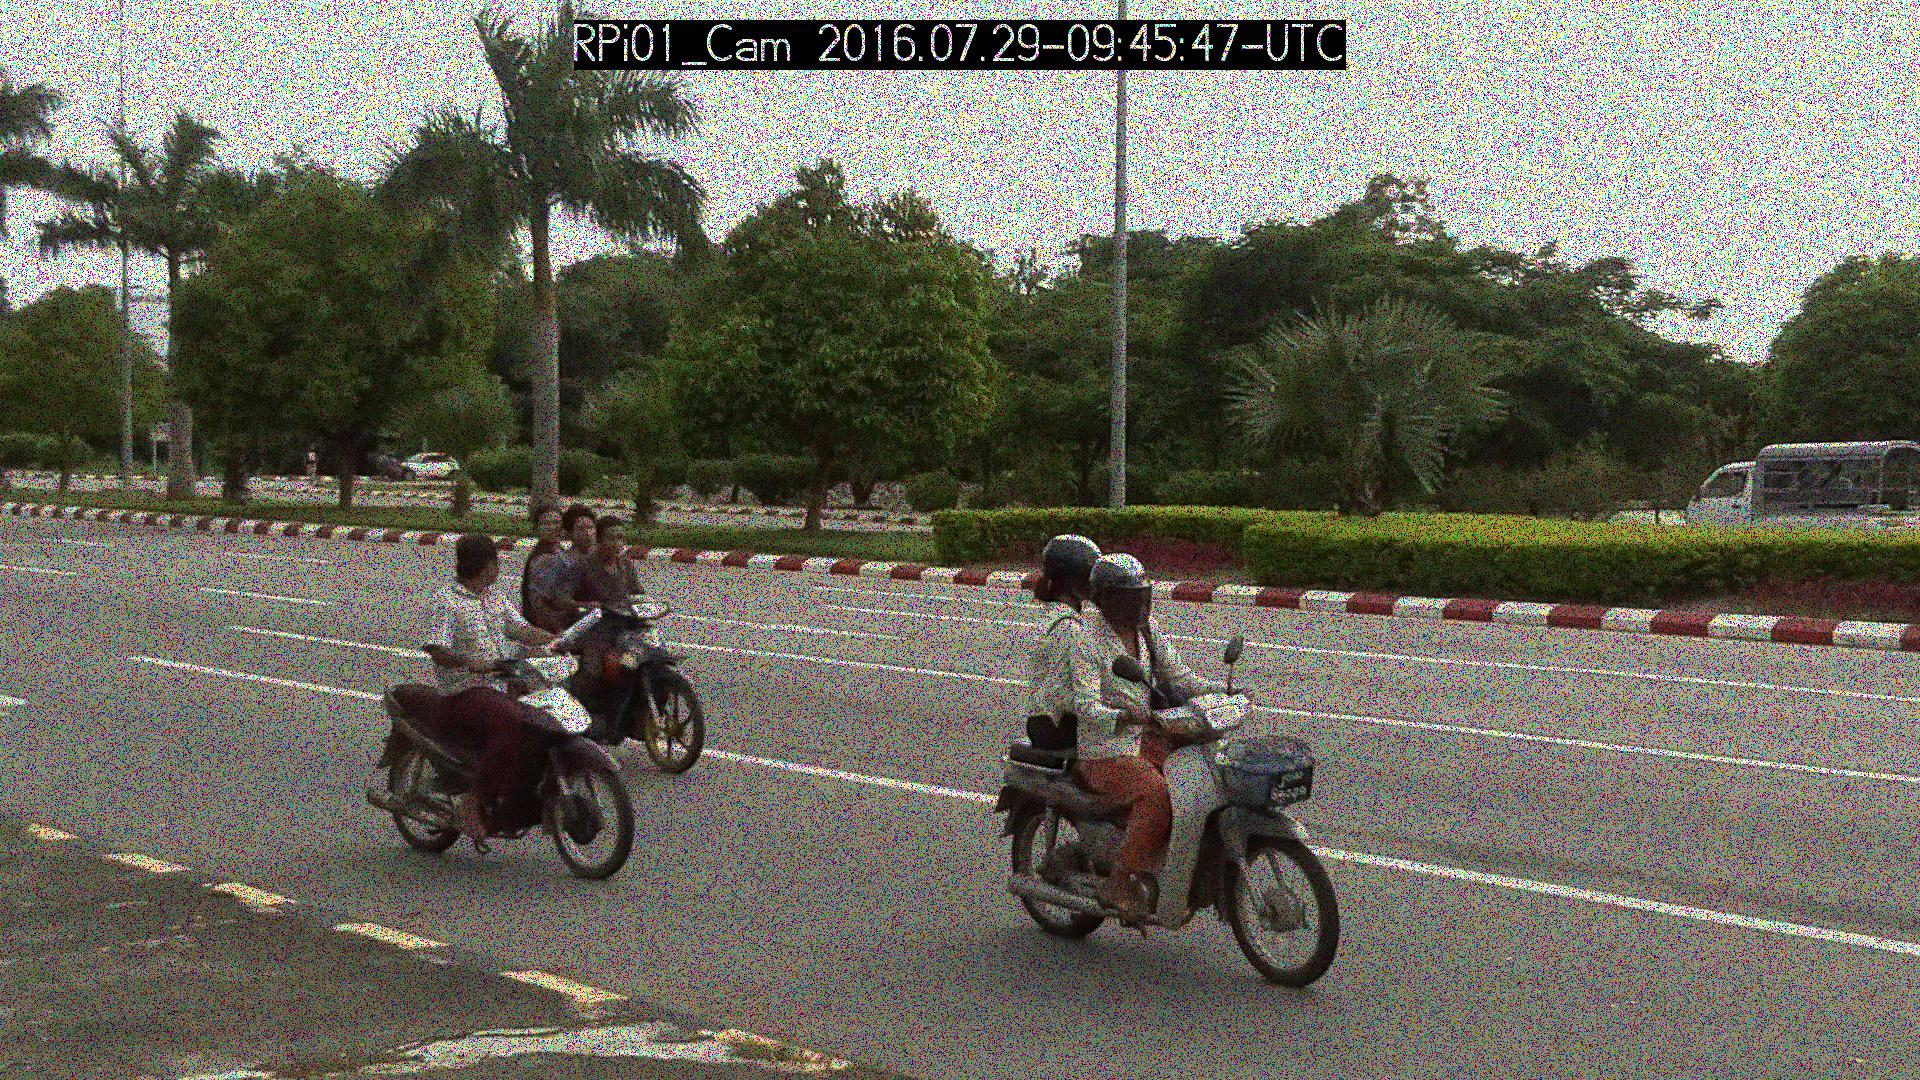
\includegraphics[width=\textwidth]{figs/chap03/pn_origin.jpg}
        \caption{pepper噪声}
        \label{fig:sub6}
    \end{subfigure}
    \caption{图像增强方式}
    \label{fig:enhance}
\end{figure}

对原数据集进行增强之后,共有6282张图片,采用7:2:1的比例对数据集进行随机划分,分别构建训练集、验证集和测试集。本文将目标类别分为18类,标签为S01-S18,其对应关系以及含义如\ref{tab:newlabel}所示,其中meaning一列命名规则为:D(Driver)代表摩托车驾驶员,P(Partner)代表乘车人员。P1代表驾驶员身后的一名乘车人员,P2代表驾驶员身后的另一名乘车人员,P0代表驾驶员身前的乘车人员(在原数据集中,某些小朋友会坐在驾驶员身前)。而D、P0、P1和P2后面紧跟着该乘车人员的头盔佩戴情况,Helmet代表已佩戴头盔,NoHelmet代表未佩戴头盔。例如,标签为S09的含义为DNoHelmetP0NoHelmetP1NoHelmet,表示摩托车驾驶员D未佩戴头盔,驾驶员身前的乘车人员P0未佩戴头盔,驾驶员身后的一名乘车人员P1未佩戴头盔。

\begin{table}[htb]
    \centering
    \caption[标签解释]{目标类别标签含义\label{tab:newlabel}}
    \begin{tabular}{lcl}
        \toprule
        \multicolumn{1}{c}{class} & \multicolumn{1}{c}{label} & \multicolumn{1}{l}{meaning} \\
        \midrule
        0 & S01 & DHelmetP1NoHelmetP2NoHelmet \\
        1 & S02 & DNoHelmetP1NoHelmetP2NoHelmet \\
        2 & S03 & DHelmetP0NoHelmetP1NoHelmet \\
        3 & S04 & DNoHelmetP1NoHelmet \\
        4 & S05 & DHelmetP0NoHelmet \\
        5 & S06 & DNoHelmet \\
        6 & S07 & DNoHelmetP1NoHelmetP2Helmet \\
        7 & S08 & DHelmetP1NoHelmet \\
        8 & S09 & DNoHelmetP0NoHelmetP1NoHelmet \\
        9 & S10 & DNoHelmetP1Helmet \\
        10 & S11 &  DHelmetP0NoHelmetP1Helmet \\
        11 & S12 &  DNoHelmetP0NoHelmetP1NoHelmetP2NoHelmet \\
        12 & S13 &  DHelmetP1NoHelmetP2Helmet \\
        13 & S14 &  DNoHelmetP0NoHelmet \\
        14 & S15 &  DHelmet \\
        15 & S16 &  DHelmetP1Helmet \\
        16 & S17 &  DHelmetP0Helmet \\
        17 & S18 &  DHelmetP1HelmetP2Helmet \\
        \bottomrule
    \end{tabular}
\end{table}

18个类别的样本数量分布如\ref{fig:label1}所示,可以看出S15标签数量最多,共6742个,其表示单一驾驶员佩戴头盔;S06标签数量次之,共6346个,其表示单一驾驶员未佩戴头盔,二者实例数量远高于其他标签。说明单一驾驶员驾驶摩托车是最常出现的情况,且佩戴头盔要比不佩戴头盔的情况稍多一些。除上述两个标签之外,S16和S04是数量最多的两个标签,S16标签共3296个,表示驾驶员和身后的一名乘客都佩戴头盔;S04标签共2503个,表示驾驶员和身后的一名乘客都未佩戴头盔。

由表中数据可以看出,单一驾驶员驾驶摩托车的情况出现次数最多,其次是驾驶员携带一名乘客的情况。并且不管是单一驾驶员,还是驾驶员携带一名乘客,佩戴头盔的情况均多于不佩戴头盔的情况。而一名驾驶员携带一名以上乘客的情况比较少见。

\begin{figure}[!htb]
    \centering
    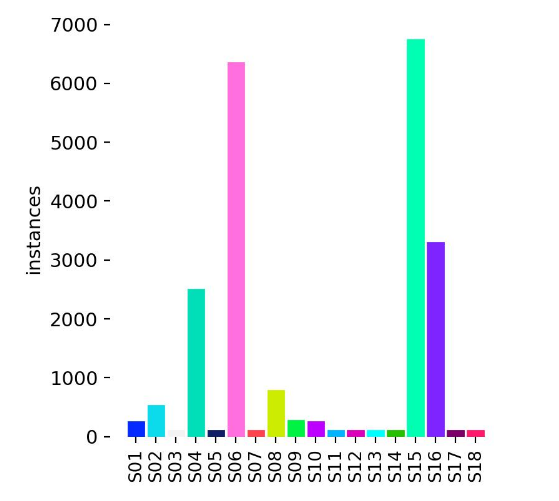
\includegraphics[width=0.8\textwidth]{figs/chap03/label1.png}
    \caption{头盔佩戴情况标签数量分布}
    \label{fig:label1}
\end{figure}

对原数据集5661张图片中的每一个驾驶员目标框进行裁剪,得到33571张包含驾驶员信息的图片,共有570个不同驾驶员。由于驾驶员的图片样本也存在不平衡的情况,对这33571张图片同样进行图像增强,保证每一个驾驶员都至少有100张样本图片。

% \begin{figure}[!htb]
%       \centering
%       \begin{minipage}{0.45\textwidth} % 调整宽度以适应需求,两张图总宽度接近1
%           \centering
%           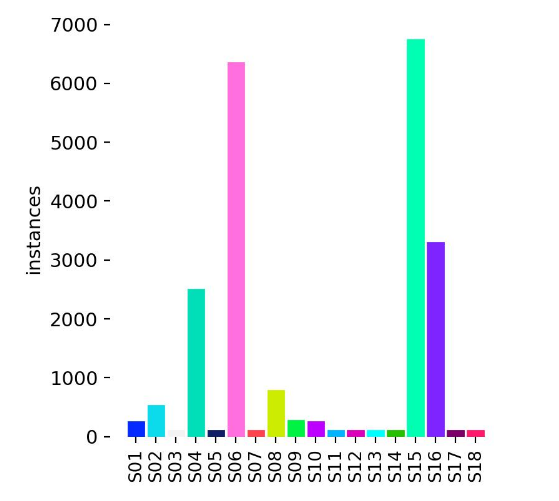
\includegraphics[width=\textwidth]{figs/chap03/label1.png}
%           \caption{头盔佩戴情况标签数量分布}
%           \label{fig:label1}
%       \end{minipage}
%       \hfill % 使两张图片之间保持一定距离
%       \begin{minipage}{0.45\textwidth}
%           \centering
%           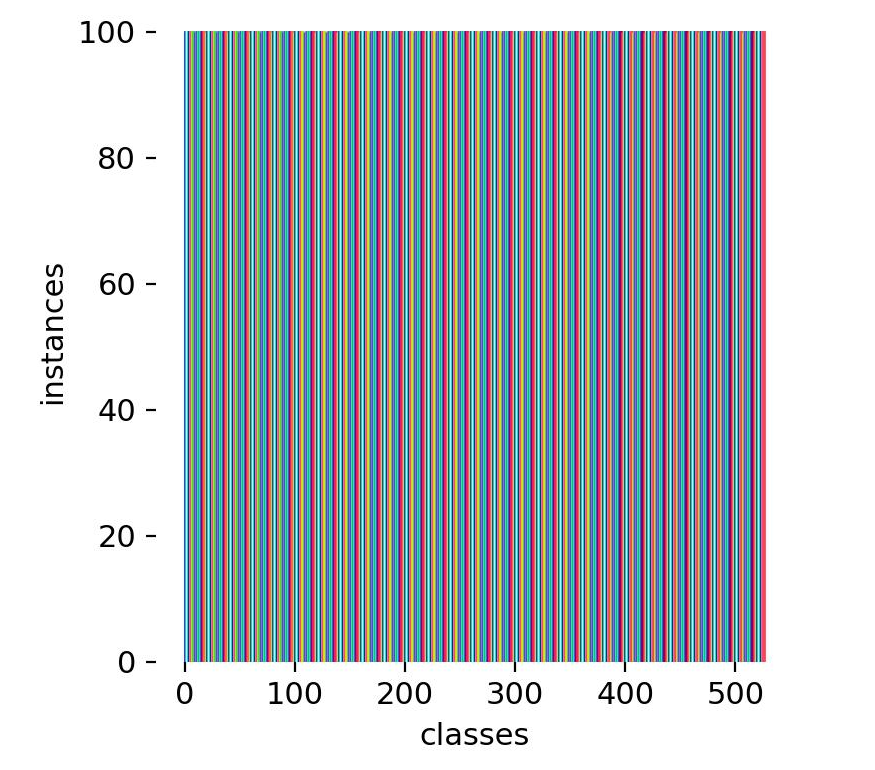
\includegraphics[width=\textwidth]{figs/chap03/label2.png}
%           \caption{驾驶员标签数量分布}
%           \label{fig:label2}
%       \end{minipage}
% \end{figure}

\section{实验环境}
操作系统:Ubuntu 20.04.3 LTS (Focal Fossa)

CPU:Intel(R) Xeon(R) Gold 5318Y CPU @ 2.10GHz

内存:1.5T

GPU:NVIDIA A40

显存:48G

CUDA版本:12.2

Pytorch版本:2.7.0+cu126

\section{参数设置}
本文分别使用YOLOv11n.pt、YOLOv11s.pt、YOLOv11m.pt进行训练,参数设置见\ref{tab:param}。本文进行头盔佩戴情况检测模型训练时,共有18个标签,在yaml文件里nc设置为18。在训练模型中,将batch设置为16,输入图像的size默认设置为640x640,epochs设置为300。
degrees设置为20,在指定度数范围内随机旋转图像,提升模型对摄像头拍摄到的不同角度的图像的识别能力。hsv\_v设置为0.6,将图像的亮度修改一部分,模拟不同的光照环境。translate设置为0.2,将图像进行水平和垂直平移,有助于检测部分可见物体。

\begin{table}[htb]
    \centering
    \caption[标签解释]{参数设置\label{tab:param}}
    \begin{tabular}{lll}
        \toprule
        \multicolumn{1}{l}{param} & \multicolumn{1}{l}{value} & \multicolumn{1}{l}{meaing}\\
        \midrule
        nc & 18 & 类别数量\\
        batch & 16 & 训练批次\\
        size & 640x640 & 输入图像的尺寸\\
        epochs & 300 & 训练轮数\\
        degrees & 20 & 控制图像随机旋转的度数范围\\
        hsv\_v & 0.6 & 控制图像亮度调整幅度\\
        translate & 0.2 & 控制图像在水平和垂直方向上的平移程度\\
        \bottomrule
    \end{tabular}
\end{table}


\section{本章小结}
本章主要介绍了原数据集的来源和本文使用到的六种数据增强方式,展示了需要训练的两个模型的标签及其数量分布。简要介绍了实验环境以及训练的参数设置,说明了本文将基于YOLOv11的三个不同量级的模型进行训练,比较各自的性能。


% % 本文件是示例论文的一部分
% % 论文的主文件位于上级目录的 `main.tex`
% \chapter{数学公式}

% 数学公式是\LaTeX{}排版中举世闻名的强项,关于数学公式的排版。在此,本文无意
% 展开讨论\LaTeX{}中的数学公式排版。只是重点说明一下由 \nwafuthesis{} 提供的
% 特有的宏。

% \section{学习资源}

% 对于数学公式的排版在\enquote{lshort-zh-cn.pdf}的第四章给出了基本的使用方法,
% 请大家阅读学习。其内容对大多数人来说已经足够用了,但是如果不能解决问题的话
% 建议大家求助于搜索引擎或者有经验的人,这也不失为一个好办法。

% 常见的几个学习\LaTeX{}数学公式排版的资源链接如下:

% \begin{itemize}
%   \item 数学排版常见问题集:
%         \url{https://www.latexstudio.net/index/details/index/mid/635}
%   \item \pkg{amsmath}手册中译:
%         \url{https://www.latexstudio.net/index/details/index/mid/706}
%   \item \LaTeX{}公式备忘单:
%         \url{https://www.latexstudio.net/index/details/index/mid/1052.html}
% \end{itemize}

% \section{公式排版与注解}

% 按我校学位论文排版要求,公式排版需要行间居中排版,公式编号按照一级标题(章)
% 连续编号(按章)并加小括号,不加导引线。类似这些细节\nwafuthesis{}模板都已进
% 行了设置。在撰写论文中只要将公式置于\env{equation}环境,并用\cs{label}命令
% 添加标签后用\cs{ref}或\cs{eqref}命令引用该公式即可。对于多行公式可以在
% \env{equation}环境中使用\env{aligned}环境实现排版。

% 需要注意的是,公式解释下面的\enquote{式中}两字需要左起顶格编排,后接符号及
% 其解释;解释顺序为先左后右,先上后下;解释与解释之间用中文分号“;”分隔。
% 此时可以用\cs{noindent}命令临时取消首行缩进,在解释完公式符号后,再次正常
% 用空行进行分段便可自动恢复段落首行缩进。

% 例如:勾股定理可以表示为\ref{eq:gougu}

% \begin{equation}
%   a^2+b^2=c^2\label{eq:gougu}
% \end{equation}

% \noindent
% 式中,$a$是一条直角边边长;$b$是另一条直角边边长;$c$是斜边边长。

% 在公式解释结束后,段落缩进应复位至首行缩进2个汉字的模式。

% \section{模板提供的数学环境}

% \nwafuthesis{} 提供了一系列预定义的数学环境,详情见\nwafuthesis{}说明书的表6。
% 其使用样例有以下7种形式。

% \subsection{axiom公理环境}

% \begin{axiom}[欧几里得距离]
% 点$\mathbf{p}$与点$\mathbf{q}$的\textbf{欧几里德距离},是连接两点的线段
% ($\overline{\mathbf{pq}}$)的长度。

% 在笛卡尔坐标系下,如果 $n$维欧几里得空间下的两个点 $\mathbf{p}=(p_1, p_2,
% \dots, p_n)$ 与点$\mathbf{q} = (q_1, q_2, q_3, \dots, q_n)$,那么点$\mathbf{p}$
% 与点$\mathbf{q}$的距离,或者点$\mathbf{q}$与点$\mathbf{p}$的距离,由
% \autoref{equ:1}定义:
% \begin{align}
% d(\mathbf{p},\mathbf{q}) = d(\mathbf{q},\mathbf{p}) & = \sqrt{(q_1-p_1)^2
%                          + (q_2-p_2)^2 + \cdots + (q_n-p_n)^2} \notag \\
% \label{equ:1}
% & = \sqrt{\sum_{i=1}^n (q_i-p_i)^2}
% \end{align}
% \end{axiom}

% \subsection{corollary推论环境}

% \begin{corollary}[欧几里得距离]
% 点$\mathbf{p}$与点$\mathbf{q}$的\textbf{欧几里德距离},是连接两点的线段
% ($\overline{\mathbf{pq}}$)的长度。

% 在笛卡尔坐标系下,如果 $n$维欧几里得空间下的两个点 $\mathbf{p}=(p_1, p_2,
% \dots, p_n)$ 与点$\mathbf{q} = (q_1, q_2, q_3, \dots, q_n)$,那么点$\mathbf{p}$
% 与点$\mathbf{q}$的距离,或者点$\mathbf{q}$与点$\mathbf{p}$的距离,由
% \autoref{equ:2}定义:
% \begin{align}
% d(\mathbf{p},\mathbf{q}) = d(\mathbf{q},\mathbf{p}) & = \sqrt{(q_1-p_1)^2
%                          + (q_2-p_2)^2 + \cdots + (q_n-p_n)^2} \notag \\
% \label{equ:2}
% & = \sqrt{\sum_{i=1}^n (q_i-p_i)^2}
% \end{align}
% \end{corollary}

% \subsection{definition定义环境}

% \begin{definition}[欧几里得距离]
% 点$\mathbf{p}$与点$\mathbf{q}$的\textbf{欧几里德距离},是连接两点的线段
% ($\overline{\mathbf{pq}}$)的长度。

% 在笛卡尔坐标系下,如果 $n$维欧几里得空间下的两个点 $\mathbf{p}=(p_1, p_2,
% \dots, p_n)$ 与点$\mathbf{q} = (q_1, q_2, q_3, \dots, q_n)$,那么点$\mathbf{p}$
% 与点$\mathbf{q}$的距离,或者点$\mathbf{q}$与点$\mathbf{p}$的距离,由
% \autoref{equ:3}定义:
% \begin{align}
% d(\mathbf{p},\mathbf{q}) = d(\mathbf{q},\mathbf{p}) & = \sqrt{(q_1-p_1)^2
%                          + (q_2-p_2)^2 + \cdots + (q_n-p_n)^2} \notag \\
% \label{equ:3}
% & = \sqrt{\sum_{i=1}^n (q_i-p_i)^2}
% \end{align}
% \end{definition}

% \subsection{example示例环境}

% \begin{example}[欧几里得距离]
% 点$\mathbf{p}$与点$\mathbf{q}$的\textbf{欧几里德距离},是连接两点的线段
% ($\overline{\mathbf{pq}}$)的长度。

% 在笛卡尔坐标系下,如果 $n$维欧几里得空间下的两个点 $\mathbf{p}=(p_1, p_2,
% \dots, p_n)$ 与点$\mathbf{q} = (q_1, q_2, q_3, \dots, q_n)$,那么点$\mathbf{p}$
% 与点$\mathbf{q}$的距离,或者点$\mathbf{q}$与点$\mathbf{p}$的距离,由
% \autoref{equ:4}定义:
% \begin{align}
% d(\mathbf{p},\mathbf{q}) = d(\mathbf{q},\mathbf{p}) & = \sqrt{(q_1-p_1)^2
%                          + (q_2-p_2)^2 + \cdots + (q_n-p_n)^2} \notag \\
% \label{equ:4}
% & = \sqrt{\sum_{i=1}^n (q_i-p_i)^2}
% \end{align}
% \end{example}

% \subsection{lemma引理环境}

% \begin{lemma}[欧几里得距离]
% 点$\mathbf{p}$与点$\mathbf{q}$的\textbf{欧几里德距离},是连接两点的线段
% ($\overline{\mathbf{pq}}$)的长度。

% 在笛卡尔坐标系下,如果 $n$维欧几里得空间下的两个点 $\mathbf{p}=(p_1, p_2,
% \dots, p_n)$ 与点$\mathbf{q} = (q_1, q_2, q_3, \dots, q_n)$,那么点$\mathbf{p}$
% 与点$\mathbf{q}$的距离,或者点$\mathbf{q}$与点$\mathbf{p}$的距离,由
% \autoref{equ:5}定义:
% \begin{align}
% d(\mathbf{p},\mathbf{q}) = d(\mathbf{q},\mathbf{p}) & = \sqrt{(q_1-p_1)^2
%                          + (q_2-p_2)^2 + \cdots + (q_n-p_n)^2} \notag \\
% \label{equ:5}
% & = \sqrt{\sum_{i=1}^n (q_i-p_i)^2}
% \end{align}
% \end{lemma}

% \subsection{proof证明环境}

% \begin{proof}[欧几里得距离]
% 点$\mathbf{p}$与点$\mathbf{q}$的\textbf{欧几里德距离},是连接两点的线段
% ($\overline{\mathbf{pq}}$)的长度。

% 在笛卡尔坐标系下,如果 $n$维欧几里得空间下的两个点 $\mathbf{p}=(p_1, p_2,
% \dots, p_n)$ 与点$\mathbf{q} = (q_1, q_2, q_3, \dots, q_n)$,那么点$\mathbf{p}$
% 与点$\mathbf{q}$的距离,或者点$\mathbf{q}$与点$\mathbf{p}$的距离,由
% \autoref{equ:6}定义:
% \begin{align}
% d(\mathbf{p},\mathbf{q}) = d(\mathbf{q},\mathbf{p}) & = \sqrt{(q_1-p_1)^2
%                          + (q_2-p_2)^2 + \cdots + (q_n-p_n)^2} \notag \\
% \label{equ:6}
% & = \sqrt{\sum_{i=1}^n (q_i-p_i)^2}
% \end{align}
% \end{proof}

% 证明与其他定理环境稍有不同, 末尾会有一个 QED 符号。

% \subsection{theorem定理环境}

% \begin{theorem}[欧几里得距离]
% 点$\mathbf{p}$与点$\mathbf{q}$的\textbf{欧几里德距离},是连接两点的线段
% ($\overline{\mathbf{pq}}$)的长度。

% 在笛卡尔坐标系下,如果 $n$维欧几里得空间下的两个点 $\mathbf{p}=(p_1, p_2,
% \dots, p_n)$ 与点$\mathbf{q} = (q_1, q_2, q_3, \dots, q_n)$,那么点$\mathbf{p}$
% 与点$\mathbf{q}$的距离,或者点$\mathbf{q}$与点$\mathbf{p}$的距离,由
% \autoref{equ:7}定义:
% \begin{align}
% d(\mathbf{p},\mathbf{q}) = d(\mathbf{q},\mathbf{p}) & = \sqrt{(q_1-p_1)^2
%                          + (q_2-p_2)^2 + \cdots + (q_n-p_n)^2} \notag \\
% \label{equ:7}
% & = \sqrt{\sum_{i=1}^n (q_i-p_i)^2}
% \end{align}
% \end{theorem}


% \section{交叉引用}

% 与图表一样,公式、定理等也需要采用专用的命令或环境进行排版以实现
% 编号、交叉引用等\emph{自动化}处理,\emph{万万不可}手动编号、引用!


% %%% Local Variables: 
% %%% mode: latex
% %%% TeX-master: "../main.tex"
% %%% End:

\chapter{实验结果与分析}

\section{评价指标}

\subsection{精度评价指标}
本文使用到的评价目标检测模型精度的指标有精度(Precision)、召回率(Recall)、平均精度(Average Precision, AP)及平均精度均值(mean Average Precision, mAP)。

% IoU用来表示预测框的准确率,它在训练阶段反映的是标注框与预测框的重合程度。例如,用A表示预测目标框,用B表示真实目标框,IoU则是A、B两个框的交集与并集的比值。IoU值越大,代表A、B两个框重叠程度越高。IoU要搭配IoU阈值一起使用。IoU阈值默认被设置为0.5,当两框的IoU大于阈值时,则判断预测框预测正确。
% 在深度学习中,将分类任务的预测结果分为以下四种,被称作混淆矩阵,见\ref{fig:matrix}:第一种是真正例(True Positive,TP),即模型预测为正例,且实际标签也是正例,预测正确;第二种是假负例(False Negative,FN),指模型预测为负例,但真实标签却是正例,预测错误;第三种是假正例(False Positive,FP),表示模型将负例误判为正例,同样是预测错误;最后一种是真负例(True Negative,TN),即模型预测为负例,同时实际标签也为负例,预测正确。这里的正例和负例其实只是针对某一类别而言的,针对A类而言,A类别就是正例,其他类别就是负例。

精度(Precision)和召回率(Recall),是衡量模型预测准确性与完整性的核心指标。精度的定义如\ref{eq:precision},其中TP表示模型预测为正例,且实际标签也是正例,FP表示模型将负例误判为正例。精度数值越大,表明FP值越小,反映出模型预测结果中真正正例的占比更高,误检更少,预测的准确性更好。召回率(Recall)的定义如\ref{eq:recall},TP同精度公式中的TP,FN表示模型漏掉的正例。召回率数值越大,代表FN值越小,说明模型对实际正例的捕捉能力更强,能够找到更多的正例样本。

% \begin{figure}[!htb]
%     \centering
%     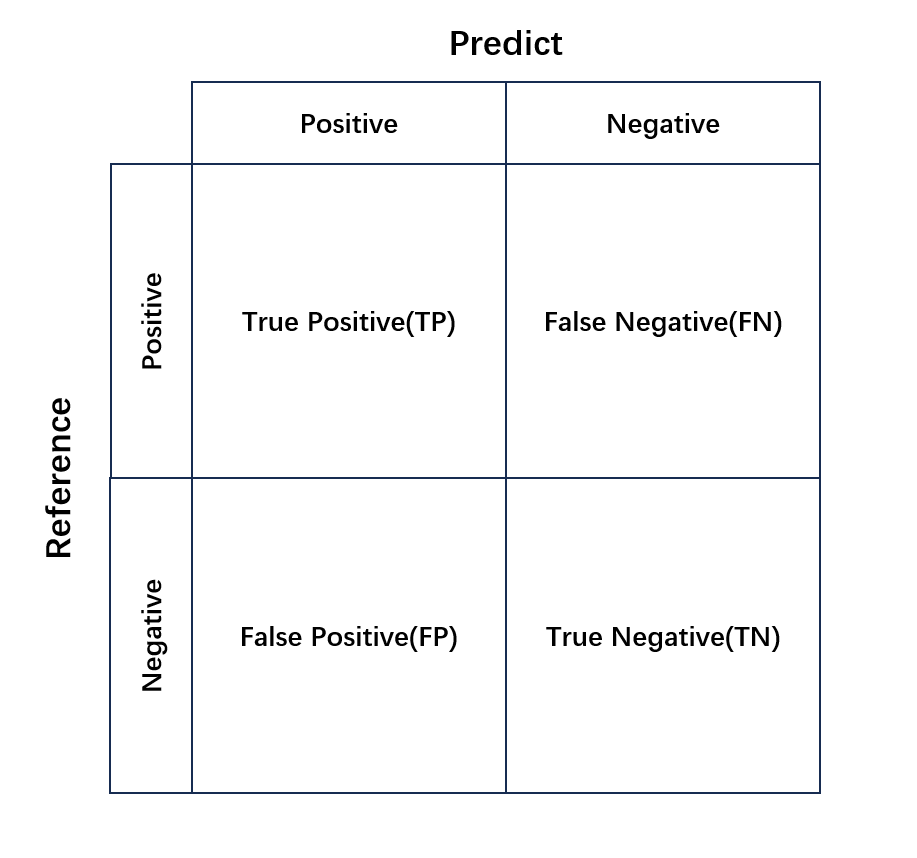
\includegraphics[width=0.6\textwidth]{figs/chap04/matrix.png}
%     \caption{混淆矩阵}
%     \label{fig:matrix}
%   \end{figure}

\begin{equation}
    \begin{aligned}
    Precision = \frac{TP}{TP + FP}\label{eq:precision}
    \end{aligned}
\end{equation}


\begin{equation}
    \begin{aligned}
    Recall = \frac{TP}{TP + FN}\label{eq:recall}
    \end{aligned}
\end{equation}

作为评估模型性能的重要指标,平均精度(AP)采用P-R曲线与坐标轴围成区域的面积进行量化表征。从几何学视角分析,较高的AP值直观体现了模型在精度和召回率两个核心评价维度上的协同优化效果,表明其既能维持较高的正样本识别准确度,又具备较强的正样本覆盖能力。在综合评价体系方面,平均精度均值(mAP)通过对所有类别的AP计算结果求均值来表征模型的整体识别准确率。YOLO模型主要采用mAP50和mAP50-95两种指标:前者设定IoU阈值为0.5时计算各类别平均精度的平均值;后者则在IoU阈值0.5至0.95范围内进行多尺度评估,最终取各阈值下mAP结果的平均值作为综合性能指标。

% \begin{figure}[!htb]
%     \centering
%     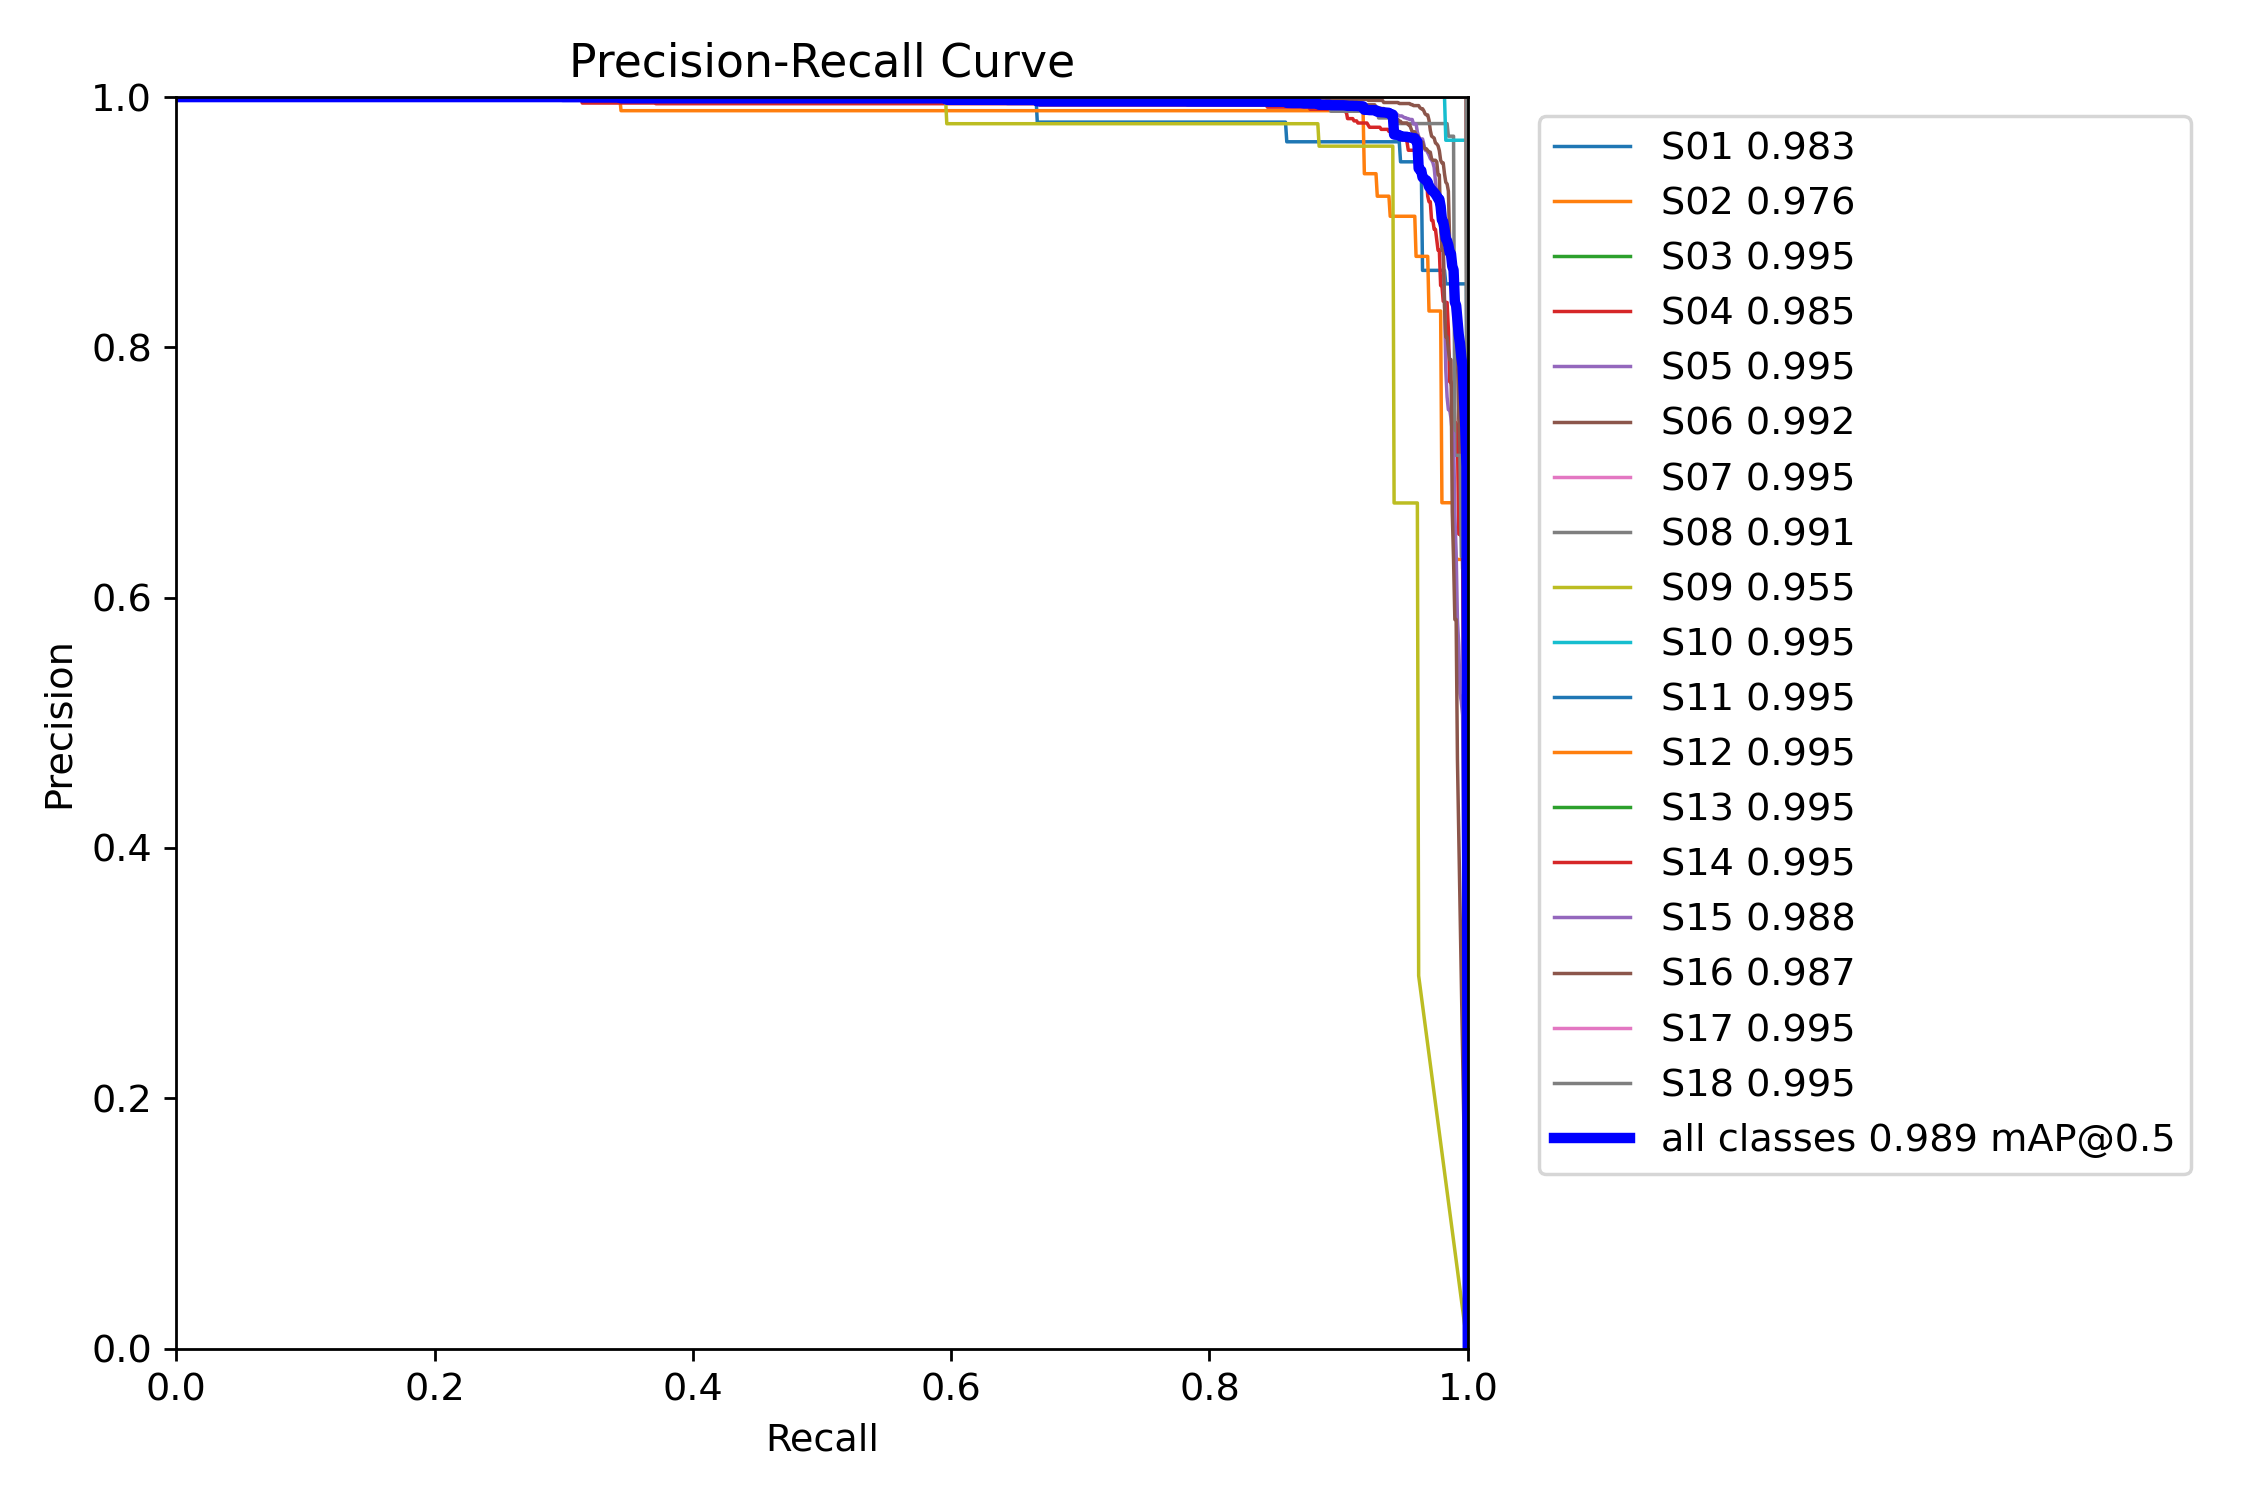
\includegraphics[width=0.6\textwidth]{figs/chap04/PR_curve.png}
%     \caption{PR曲线}
%     \label{fig:pr}
%   \end{figure}

\subsection{速度评价指标}
本文采用每秒帧率(FPS)与浮点运算量(FLOPs)作为目标检测模型速度性能的量化评估指标。其中,FPS指标反映了模型在单位时间内能够检测的图像帧数,其数值越高,意味着一秒内能执行更多的目标检测任务;而FLOPs则用于量化模型执行目标检测任务过程中所涉及的浮点运算次数,该指标能够有效表征模型的计算量,FLOPs越低,理论速度越快,但并不直接等于实际速度。

\section{实验结果分析}
\subsection{头盔佩戴情况模型}
本文基于YOLOv11n、YOLOv11s和YOLOv11m三个模型,各训练了300个epoch,头盔佩戴情况模型训练结果如\ref{fig:helmetResult_part1}和\ref{fig:helmetResult_part2}所示。下面对边界框回归损失、分类损失、分布损失、精度、召回率、mAP50和mAP50-95这七个指标进行详细对比分析。
\begin{figure}[H]
    \centering
    \begin{subfigure}[t]{0.43\textwidth}
        \centering
        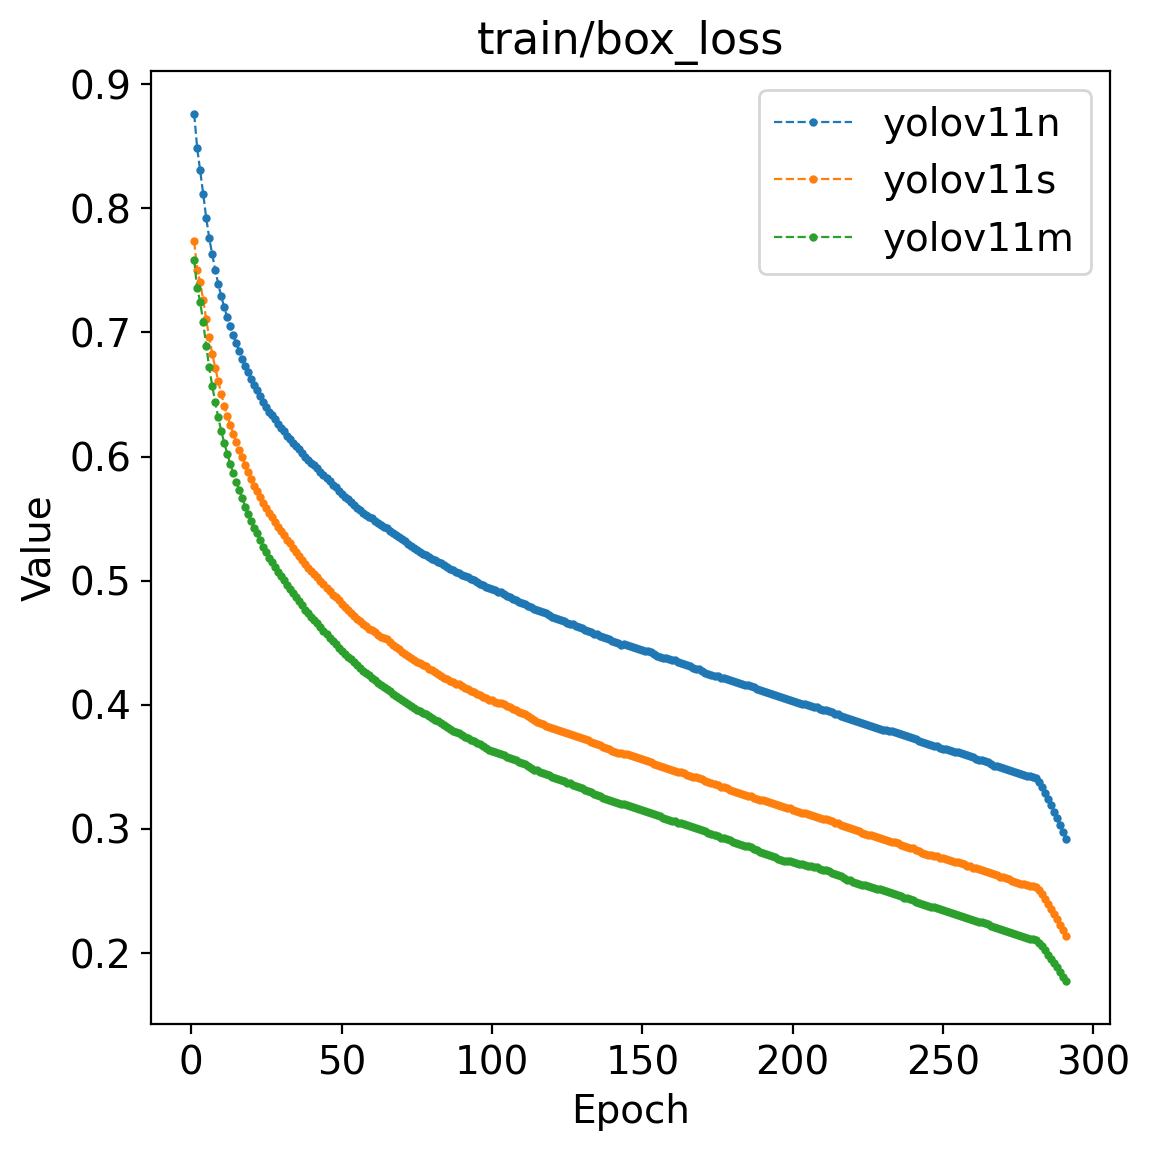
\includegraphics[width=\textwidth]{figs/chap04/helmet_result/helmet_train_box_loss.png}
        \caption{训练集边界框回归损失}
        \label{fig:helmet_train_box_loss}
    \end{subfigure}
    \begin{subfigure}[t]{0.43\textwidth}
        \centering
        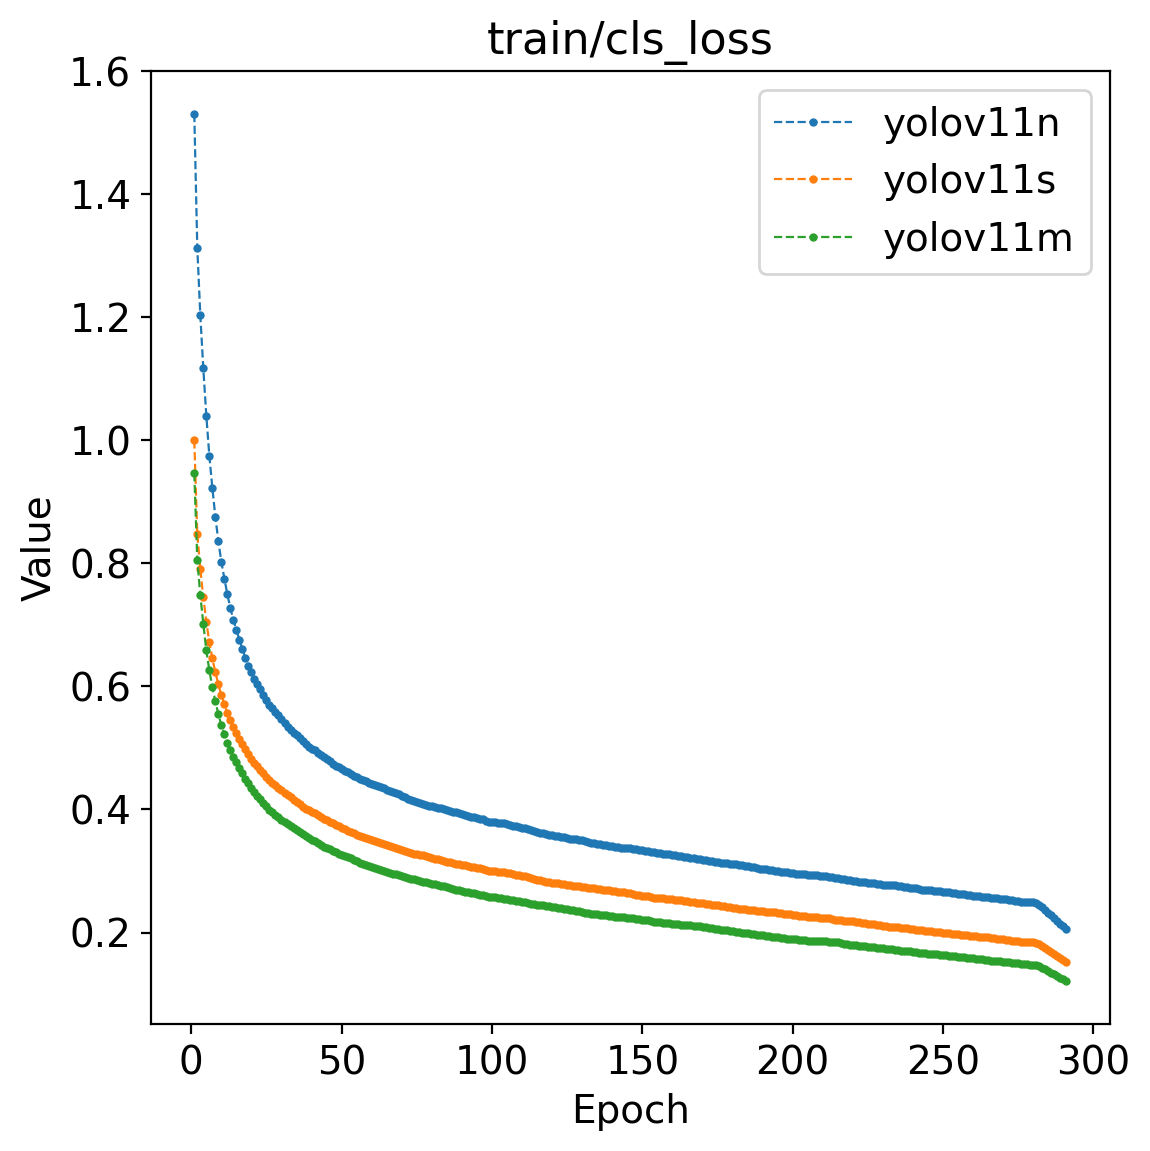
\includegraphics[width=\textwidth]{figs/chap04/helmet_result/helmet_train_cls_loss.png}
        \caption{训练集分类损失}
        \label{fig:helmet_train_cls_loss}
    \end{subfigure}
    \begin{subfigure}[t]{0.43\textwidth}
        \centering
        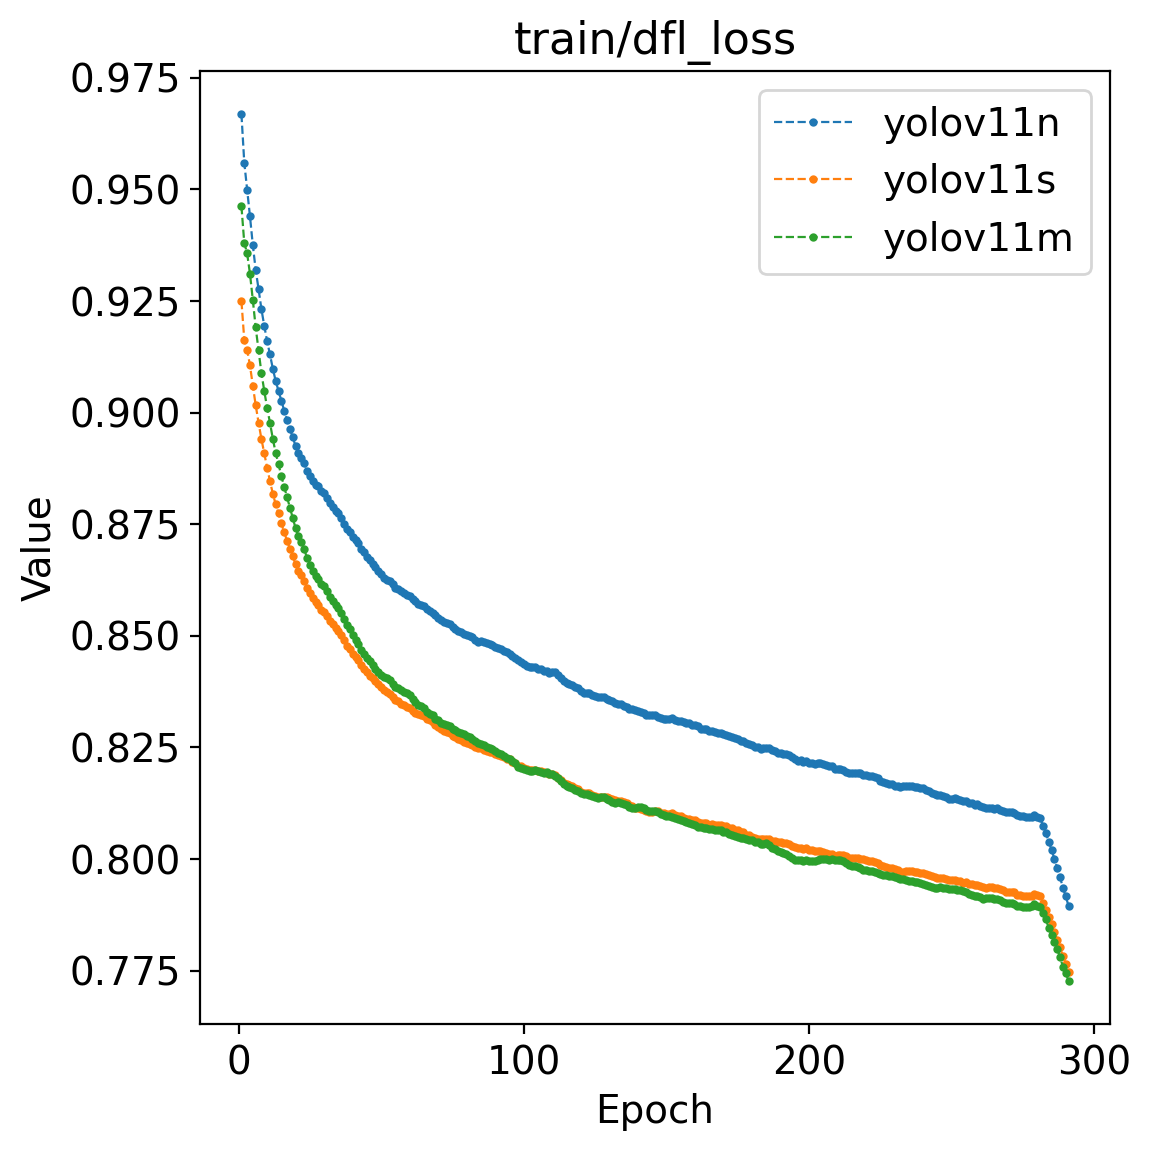
\includegraphics[width=\textwidth]{figs/chap04/helmet_result/helmet_train_dfl_loss.png}
        \caption{训练集分布损失}
        \label{fig:helmet_train_dfl_loss}
    \end{subfigure}
    \begin{subfigure}[t]{0.43\textwidth}
        \centering
        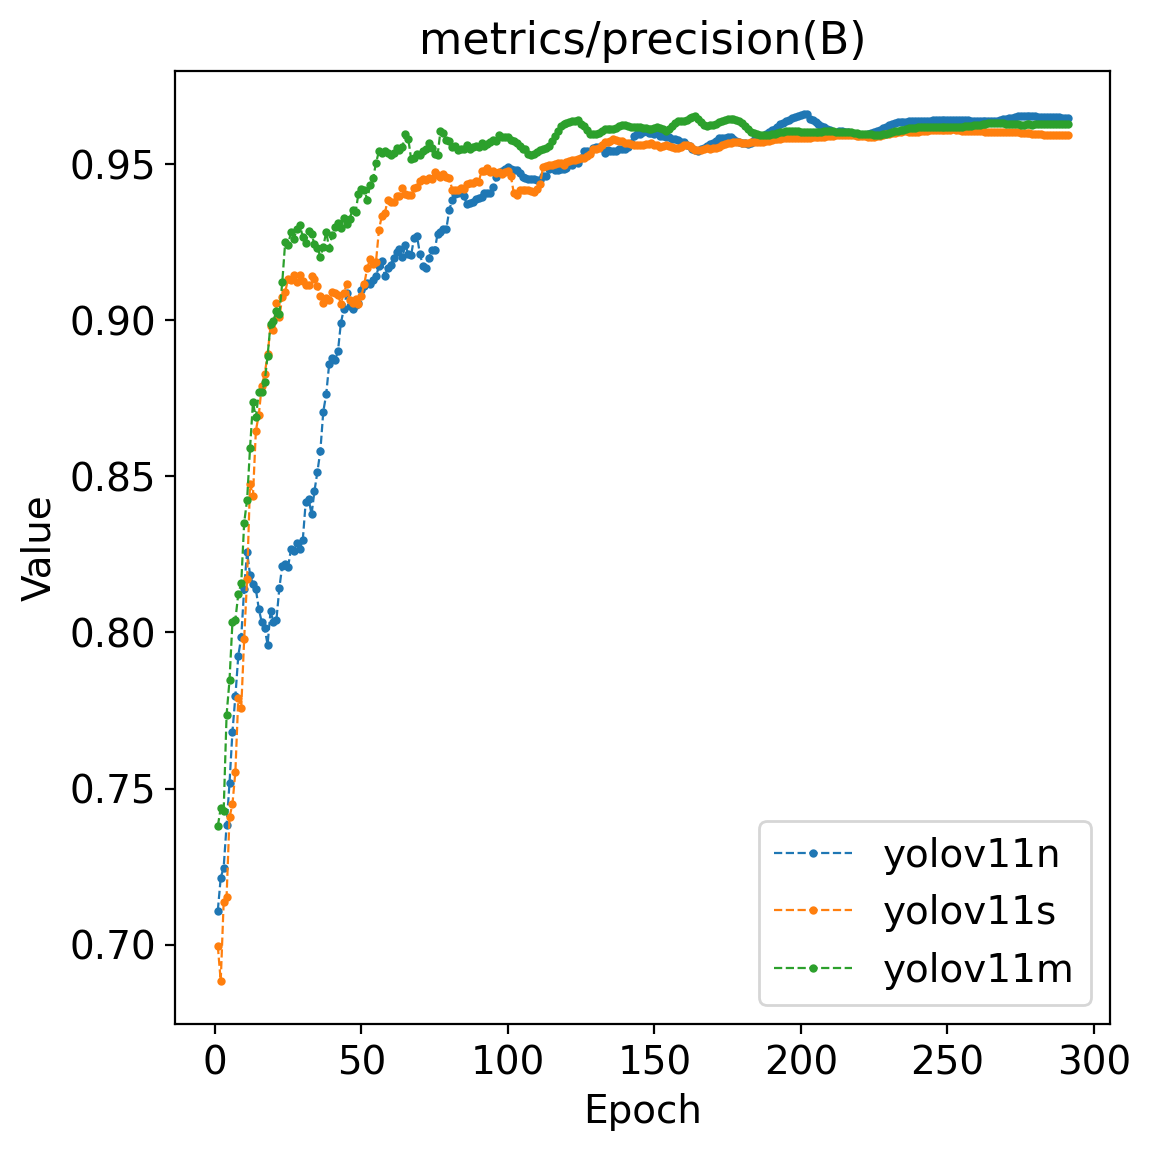
\includegraphics[width=\textwidth]{figs/chap04/helmet_result/helmet_metrics_precision(B).png}
        \caption{精度}
        \label{fig:helmet_metrics_precision}
    \end{subfigure}
    \caption{头盔佩戴情况模型训练结果(第一部分)}
    \label{fig:helmetResult_part1}
\end{figure}

\newpage % 这里使用 \newpage 强制分页

\begin{figure}[H]
    \centering
    \begin{subfigure}[t]{0.43\textwidth}
        \centering
        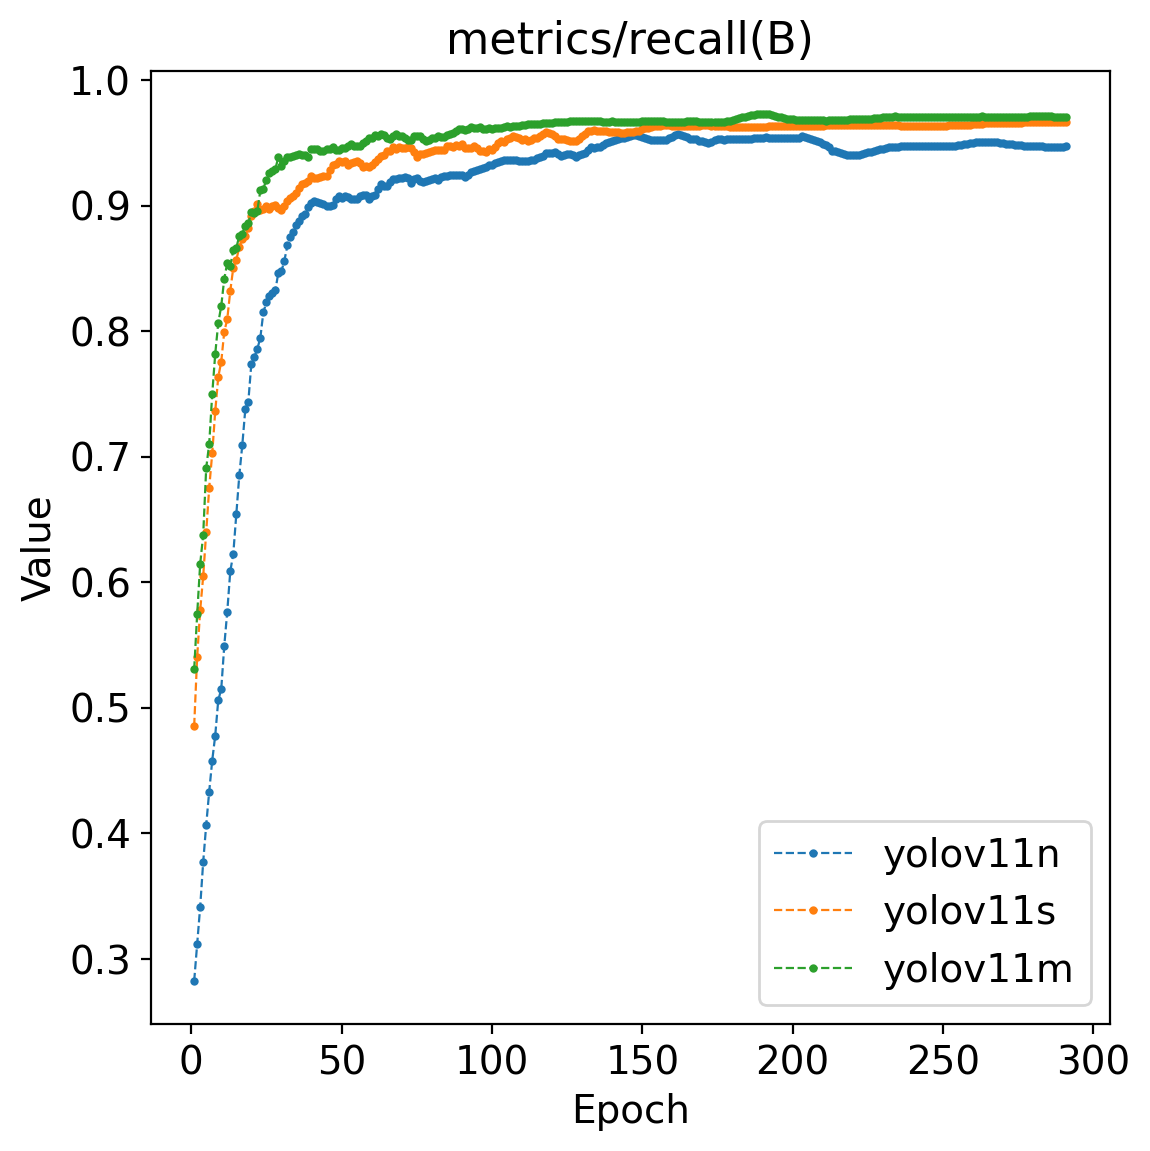
\includegraphics[width=\textwidth]{figs/chap04/helmet_result/helmet_metrics_recall(B).png}
        \caption{召回率}
        \label{fig:helmet_metrics_recall}
    \end{subfigure}
    \begin{subfigure}[t]{0.43\textwidth}
        \centering
        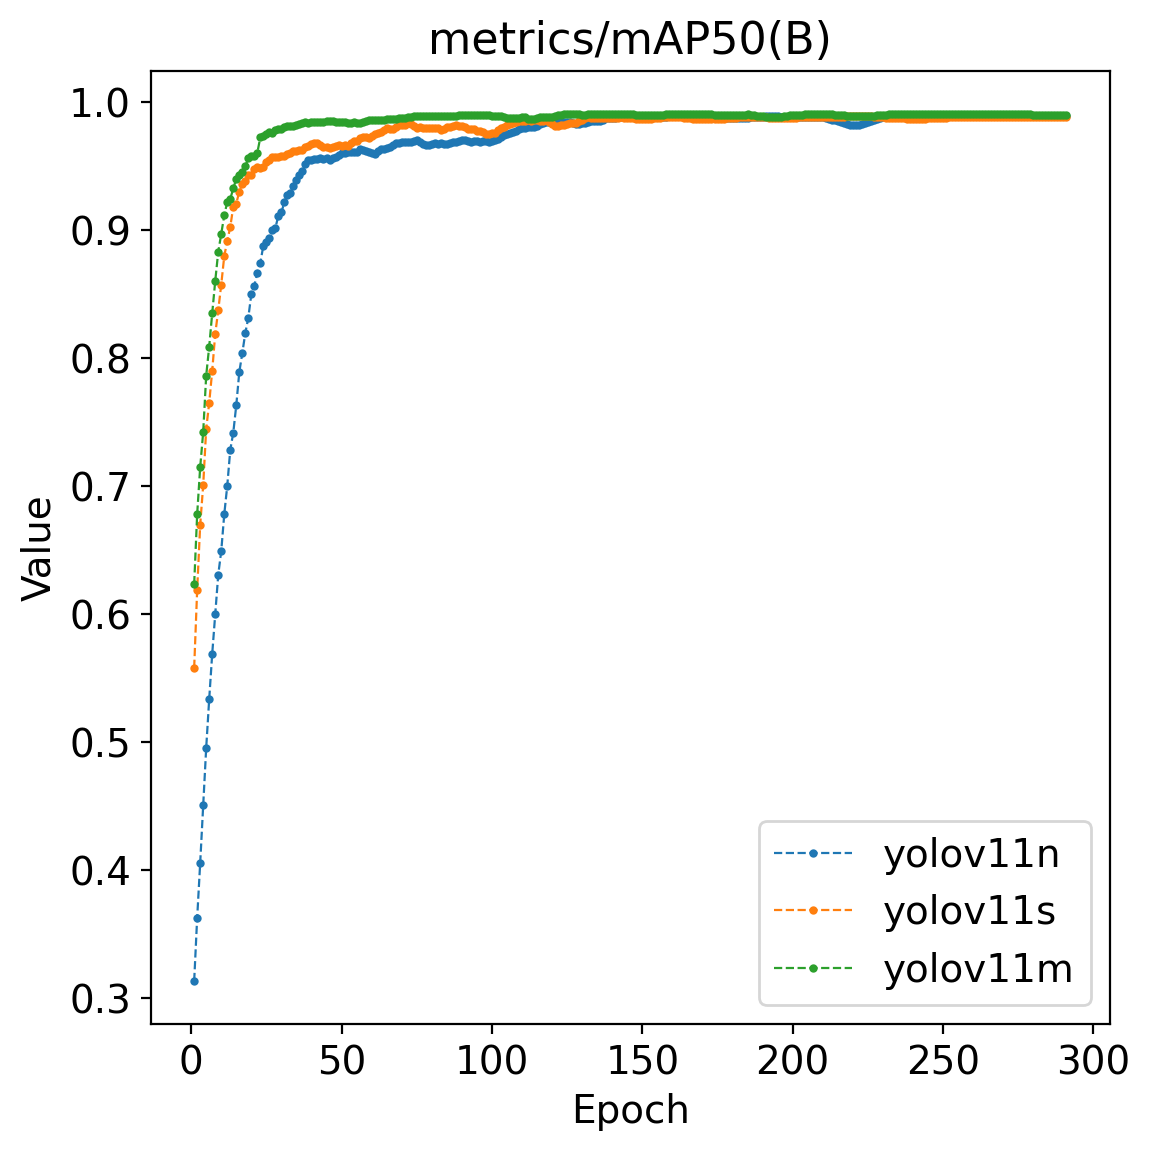
\includegraphics[width=\textwidth]{figs/chap04/helmet_result/helmet_metrics_mAP50(B).png}
        \caption{mAP50}
        \label{fig:helmet_metrics_mAP50}
    \end{subfigure}
    \begin{subfigure}[t]{0.43\textwidth}
        \centering
        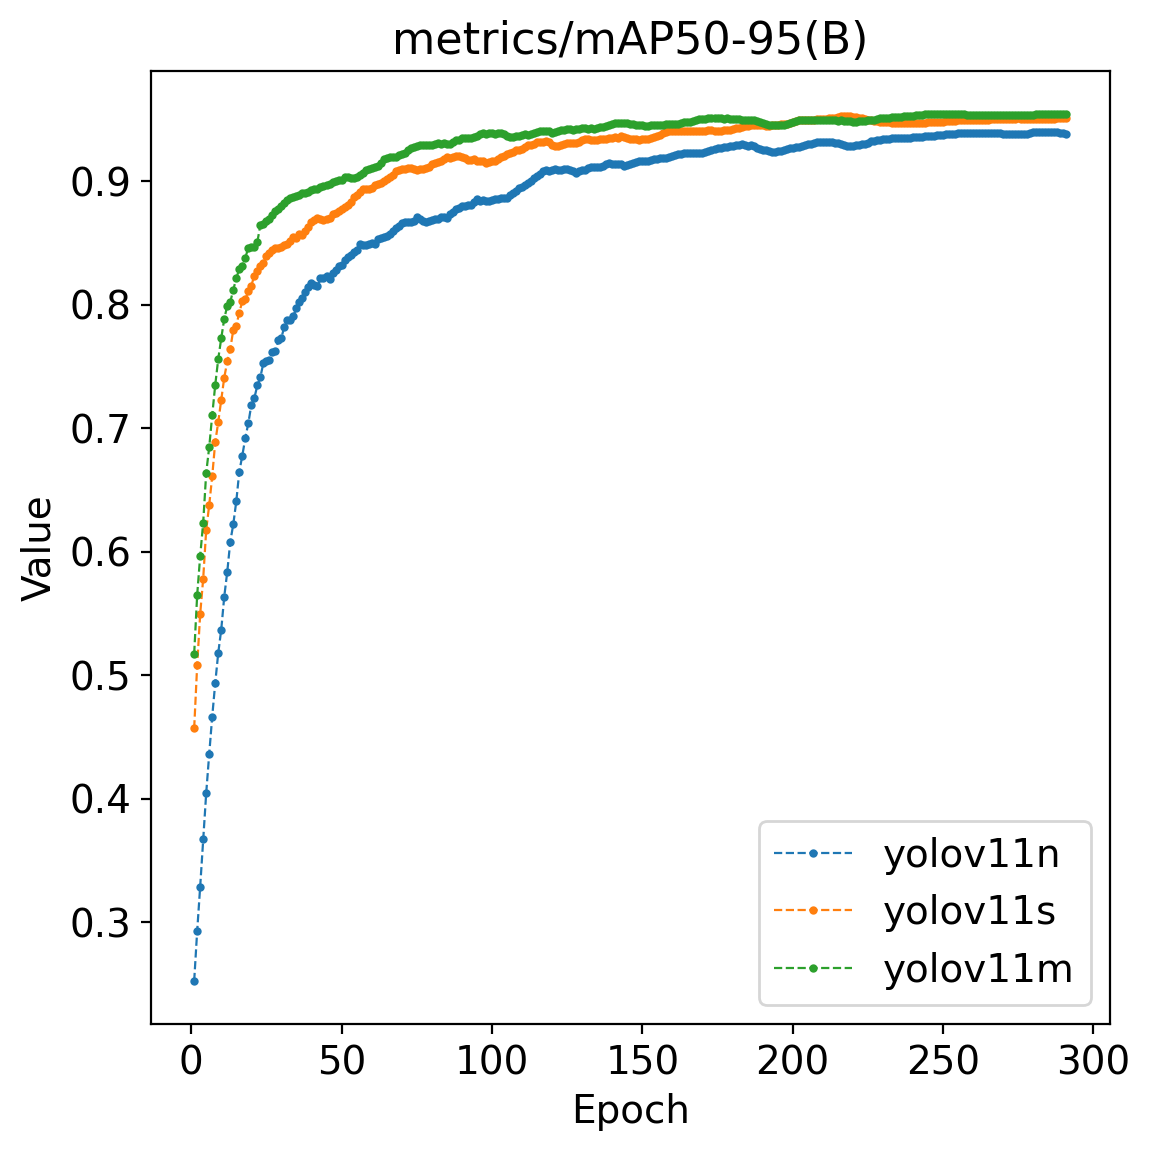
\includegraphics[width=\textwidth]{figs/chap04/helmet_result/helmet_metrics_mAP50-95(B).png}
        \caption{mAP50-95}
        \label{fig:helmet_metrics_mAP50-95}
    \end{subfigure}
    \begin{subfigure}[t]{0.43\textwidth}
        \centering
        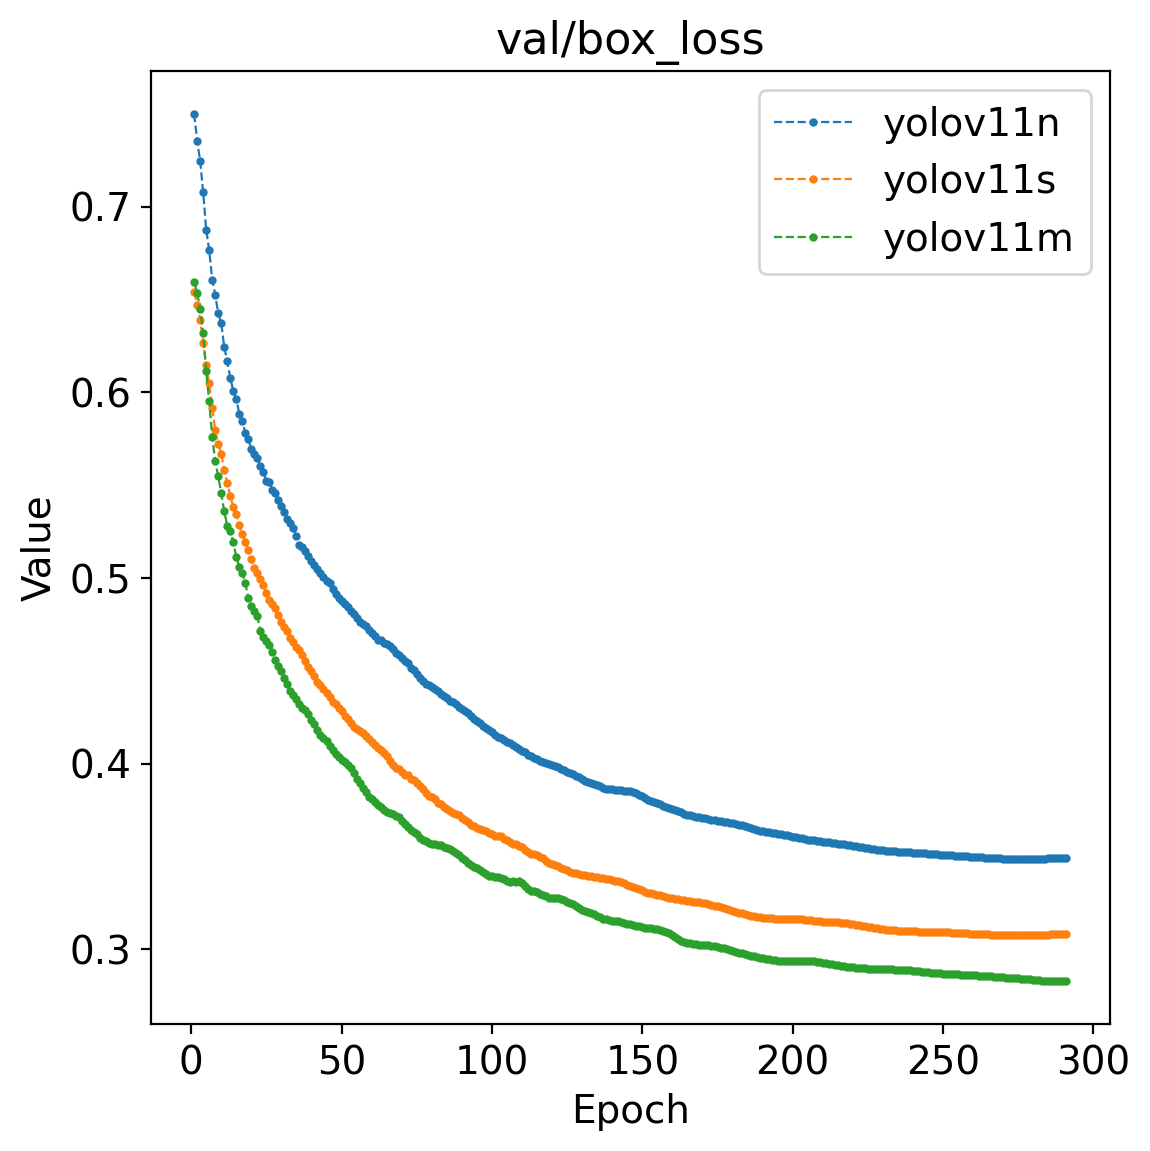
\includegraphics[width=\textwidth]{figs/chap04/helmet_result/helmet_val_box_loss.png}
        \caption{验证集边界框回归损失}
        \label{fig:helmet_val_box_loss}
    \end{subfigure}
    \begin{subfigure}[t]{0.43\textwidth}
        \centering
        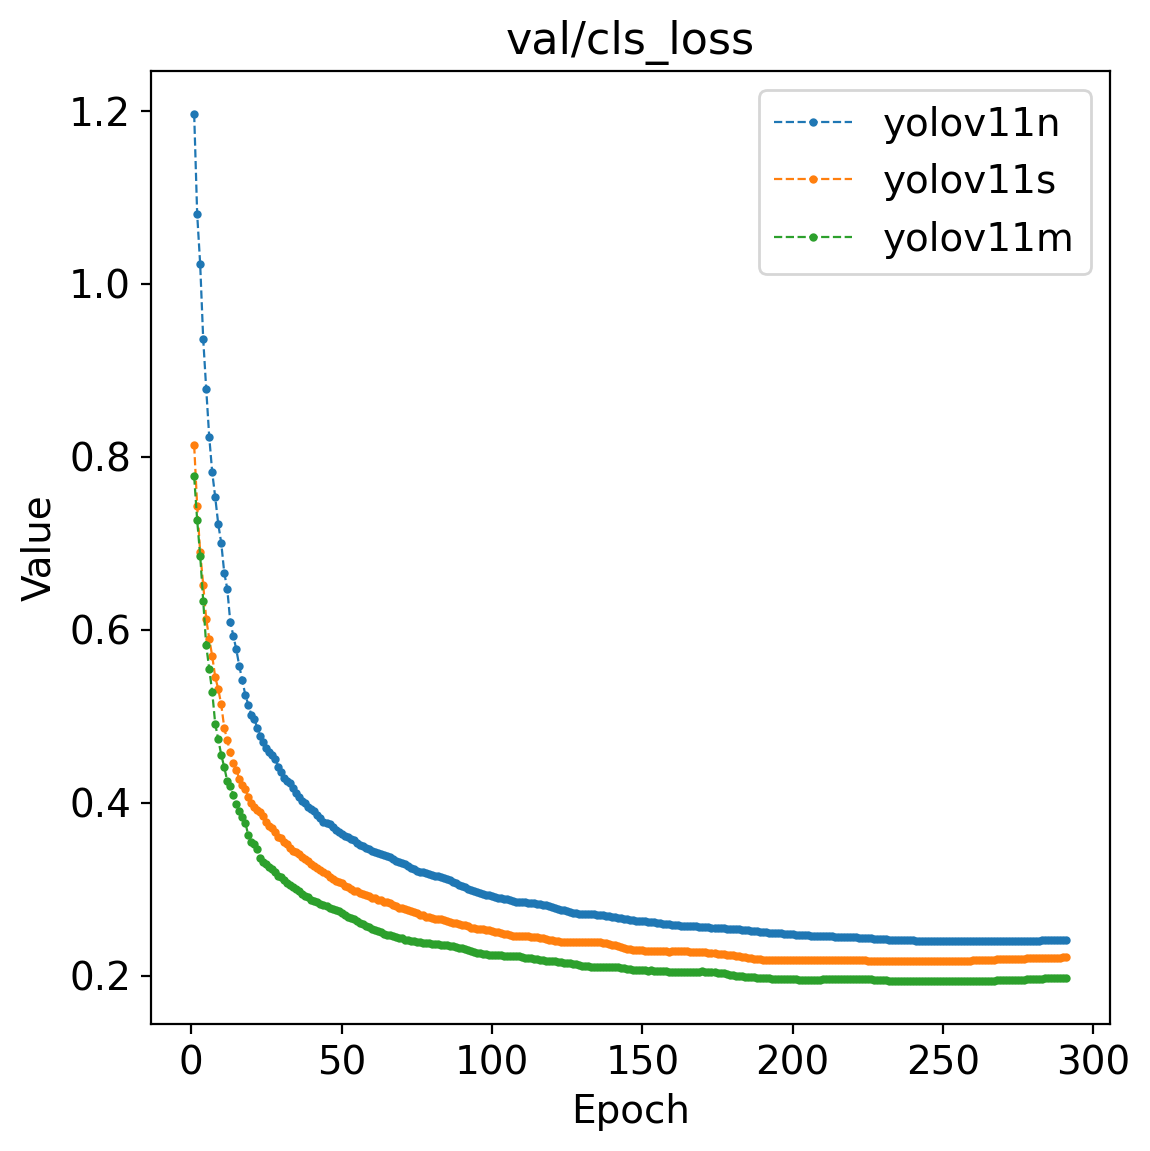
\includegraphics[width=\textwidth]{figs/chap04/helmet_result/helmet_val_cls_loss.png}
        \caption{验证集分类损失}
        \label{fig:helmet_val_cls_loss}
    \end{subfigure}
    \begin{subfigure}[t]{0.43\textwidth}
        \centering
        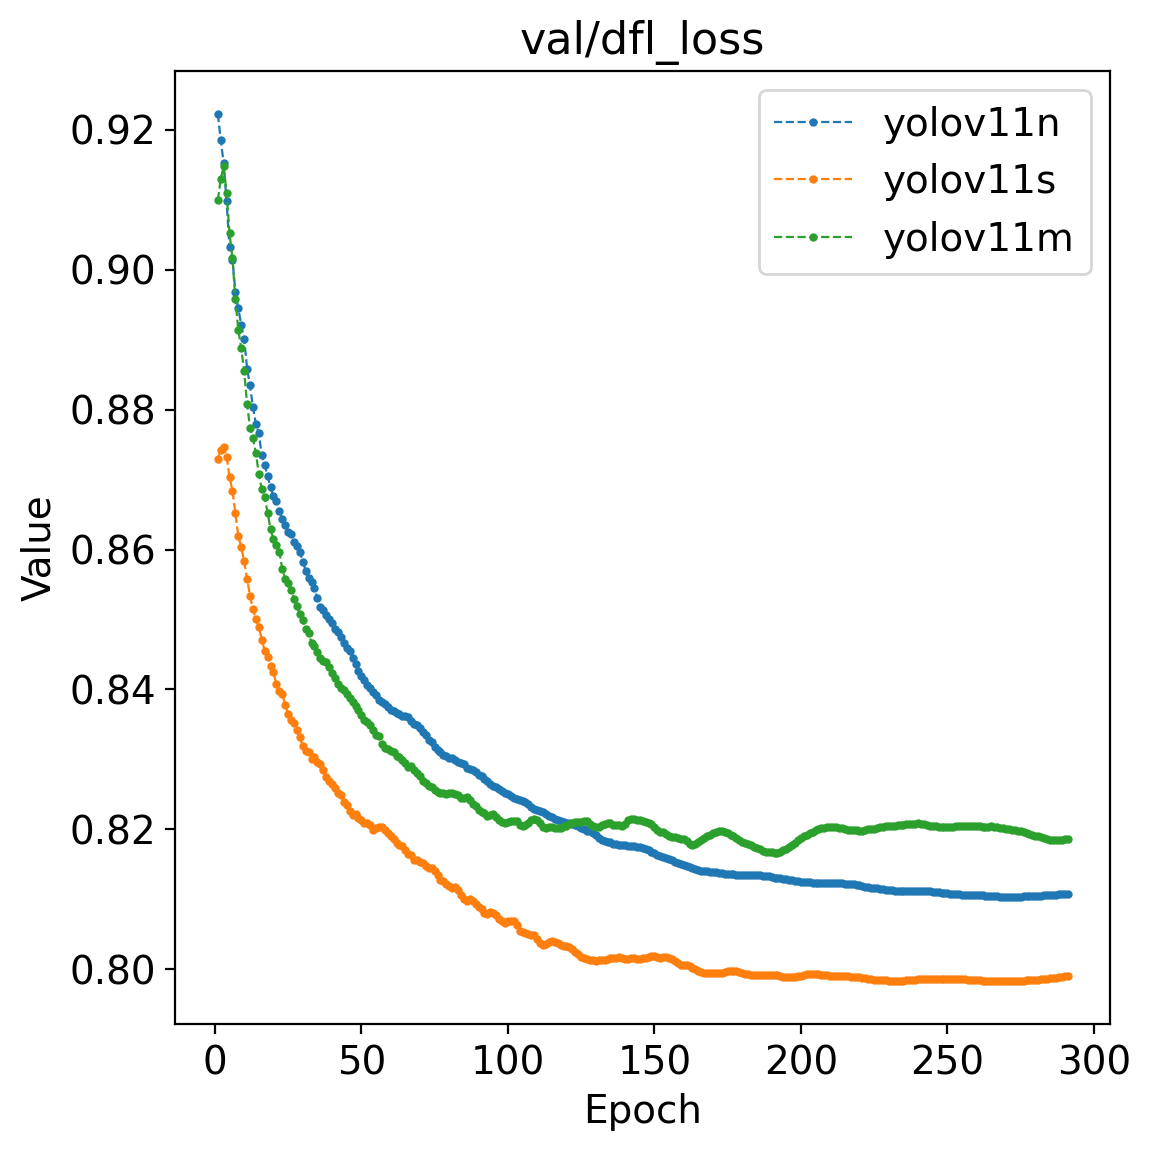
\includegraphics[width=\textwidth]{figs/chap04/helmet_result/helmet_val_dfl_loss.png}
        \caption{验证集分布损失}
        \label{fig:helmet_val_dfl_loss}
    \end{subfigure}
    \caption{头盔佩戴情况模型训练结果(第二部分)}
    \label{fig:helmetResult_part2}
\end{figure}
% \begin{figure}[H]
%     \centering
%     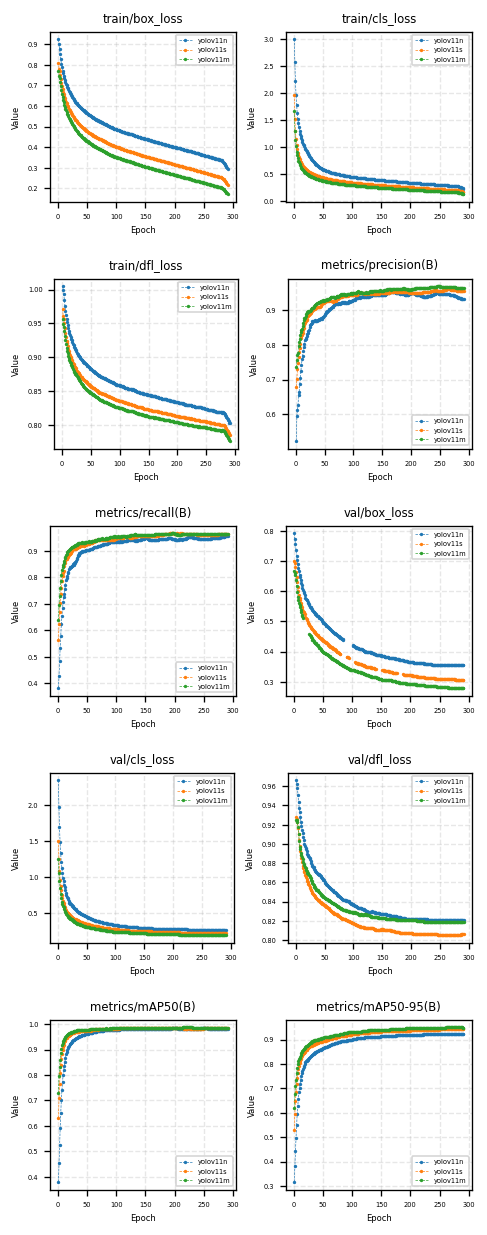
\includegraphics[width=1\textwidth]{figs/chap04/YoloMetrics_Combined.png}
%     \caption{头盔佩戴情况模型训练结果}
%     \label{fig:helmetResult}
% \end{figure}

边界框回归损失:三个模型的边界框回归损失值在训练过程中逐渐降低。YOLOv11n下降趋势相对较缓,YOLOv11s和YOLOv11m前期下降速度较快且相近,在训练进行大约50轮之后,YOLOv11m下降速度略快于YOLOv11s,说明YOLOv11m在边界框回归损失的收敛上最具优势。在训练后期,YOLOv11m的边界框回归损失最终值最低,YOLOv11s次之,YOLOv11n相对较高。这表明YOLOv11m在边界框定位的准确性上表现更好。

分类损失:三个模型分类损失收敛趋势相似,均在前期快速下降,后期平稳下降。前期YOLOv11n下降稍快,YOLOv11s与YOLOv11m相近。中期YOLOv11s和YOLOv11m的下降速度与YOLOv11n相似,后期三者收敛速度相近。
YOLOv11m最终的分类损失值最低,YOLOv11s和YOLOv11n相对较高且较为接近,意味着YOLOv11m在分类任务上的准确性更高。

分布损失:YOLOv11s与YOLOv11m整体收敛趋势相似,前期都比YOLOv11n收敛速度略快,后期三者收敛速度近似。YOLOv11s与YOLOv11m达到的最优值近乎相同,且都比YOLOv11n的最优值更好。

精度:三个模型精度均随训轮数增多逐渐变高。YOLOv11s和YOLOv11m前期上升速度较快且相近,YOLOv11n稍慢;后期三者趋势相似。YOLOv11m达到的精度最优值最高,YOLOv11s次之,YOLOv11n相对较低,表明YOLOv11m在预测准确程度上表现更优。

召回率:YOLOv11s与YOLOv11m前期收敛趋势相同且均比YOLOv11n收敛速度快;后期三个模型的召回率收敛速度都逐渐趋于平稳。YOLOv11m召回率最优值最高,YOLOv11s与之接近,YOLOv11n相对较低。说明YOLOv11m在捕捉正例样本能力上表现最好。

mAP50:YOLOv11s和YOLOv11m的mAP50值在训练前期上升迅速,YOLOv11n稍慢;中后期YOLOv11m率先趋于稳定,YOLOv11s次之。最后三个模型得到的mAP50最优值近似。

mAP50-95:YOLOv11s和YOLOv11m前期收敛速度快且相近,YOLOv11n比较缓慢;后期YOLOv11m收敛更平稳,更快达到较高精度水平。YOLOv11m的mAP50-95最优值最高,YOLOv11s与之相近,YOLOv11n较低。表明YOLOv11m与YOLOv11s在不同IoU阈值下平均精度综合表现都比较好。

根据训练结果中的csv文件,能够得到各项指标在每一轮训练中的精确值,上述指标在训练过程中的最优值的对比如\ref{tab:modelCompare1}所示。从表格呈现的趋势来看,随着模型规模增大,三个损失函数的收敛速度更快,最终达到的损失值更低。其余四项指标,除检测精度外都随模型规模增大表现更优。

\begin{table}[htb]
    \centering
    \caption[目标数据]{模型损失函数与检测精度指标对比1\label{tab:modelCompare1}}
    \begin{tabular}{lccccccc}
        \toprule
        Model & 
        \makecell{box\_loss\\(\%)} & 
        \makecell{cls\_loss\\(\%)} & 
        \makecell{dfl\_loss\\(\%)} & 
        \makecell{Precision\\(\%)} & 
        \makecell{Recall\\(\%)} & 
        \makecell{mAP50\\(\%)} & 
        \makecell{mAP50-95\\(\%)} \\
        \midrule
        YOLOv11n & 28.4 & 20.2 & 78.6 & 96.7 & 96.6 & 99.0 & 94.1 \\
        YOLOv11s & 20.5 & 14.7 & 77.2 & 96.2 & 97.2 & 99.0 & 95.4 \\
        YOLOv11m & 17.1 & 11.8 & 77.1 & 97.3 & 98.1 & 99.1 & 95.5 \\
        \bottomrule
    \end{tabular}
\end{table}


除了检测精度,模型的推理速度与计算复杂度同样是衡量性能的关键要素,\ref {tab:speedCompare1}对比了YOLOv11n、YOLOv11s和YOLOv11m三个版本基于实测数据的FPS与FLOPs数值。对于FPS指标,YOLOv11n的值最高,达到41.67,意味着该模型每秒能够处理41.67帧图像,实时性最强;YOLOv11s的FPS为36.63,仅次于YOLOv11n;YOLOv11m的FPS最低,为31.75。由此可见,随着模型规模增大(从n到m),检测速度逐渐降低,因为更大的模型通常包含更多的参数和计算操作,需要更长的推理时间。对于FLOPs指标,YOLOv11m的FLOPs值最高,为68.26G,表明其完成一次前向推理所需的浮点运算次数最多,计算复杂度最高;YOLOv11s的FLOPs为21.59G;而YOLOv11n的 FLOPs最低,仅为6.4G。综合两项指标来看,YOLOv11模型的检测精度与计算速度呈现负相关性。YOLOv11n在检测精度上略逊于其他版本,但其计算复杂度低、检测速度快;而YOLOv11m推理速度较慢,计算量最大,但有更高的检测精度。

\begin{table}[htb]
    \centering
    \caption[目标数据]{模型检测速度对比1\label{tab:speedCompare1}}
    \begin{tabular}{lcc}
        \toprule
        Model & 
        \makecell{FPS(1)} & 
        \makecell{FLOPs(G)} \\
        \midrule
        YOLOv11n & 41.67 & 6.4 \\
        YOLOv11s & 36.63 & 21.59 \\
        YOLOv11m & 31.75 & 68.26 \\
        \bottomrule
    \end{tabular}
\end{table}

% 6.46G 21.59G 68.26G   24 27.3 31.5

三个模型的混淆矩阵如\ref{fig:nmatrix}、\ref{fig:smatrix}、\ref{fig:mmatrix}所示。YOLOv11n对S07类别的检测效果较差,有33\%的错误预测情况。对S09类别有6\%的误判和6\%的漏检。对剩余标签的检测准确度都在94\%以上。YOLOv11s相较于YOLOv11n,对S07和S09两个标签的检测准确度有大幅提升,且对所有标签的检测精度都在94\%以上。YOLOv11m相较于YOLOv11n,对各类别的检测精度近似,没有大幅变化,且对所有标签的检测精度也都在94\%以上。

综合上文对三个模型在检测精度、检测速度和混淆矩阵三个方面的对比,YOLOv11n模型优势是检测速度快,适用于实时检测场景;YOLOv11s模型在检测精度、检测速度和计算复杂度方面取得了平衡,适用于对实时性和精度都有一定要求的场景;YOLOv11m模型牺牲了一定的检测速度,并且资源开销巨大,但换来了更高的精度,能够更准确地识别驾乘人员的头盔佩戴情况。

\begin{figure}[H]
    \centering
    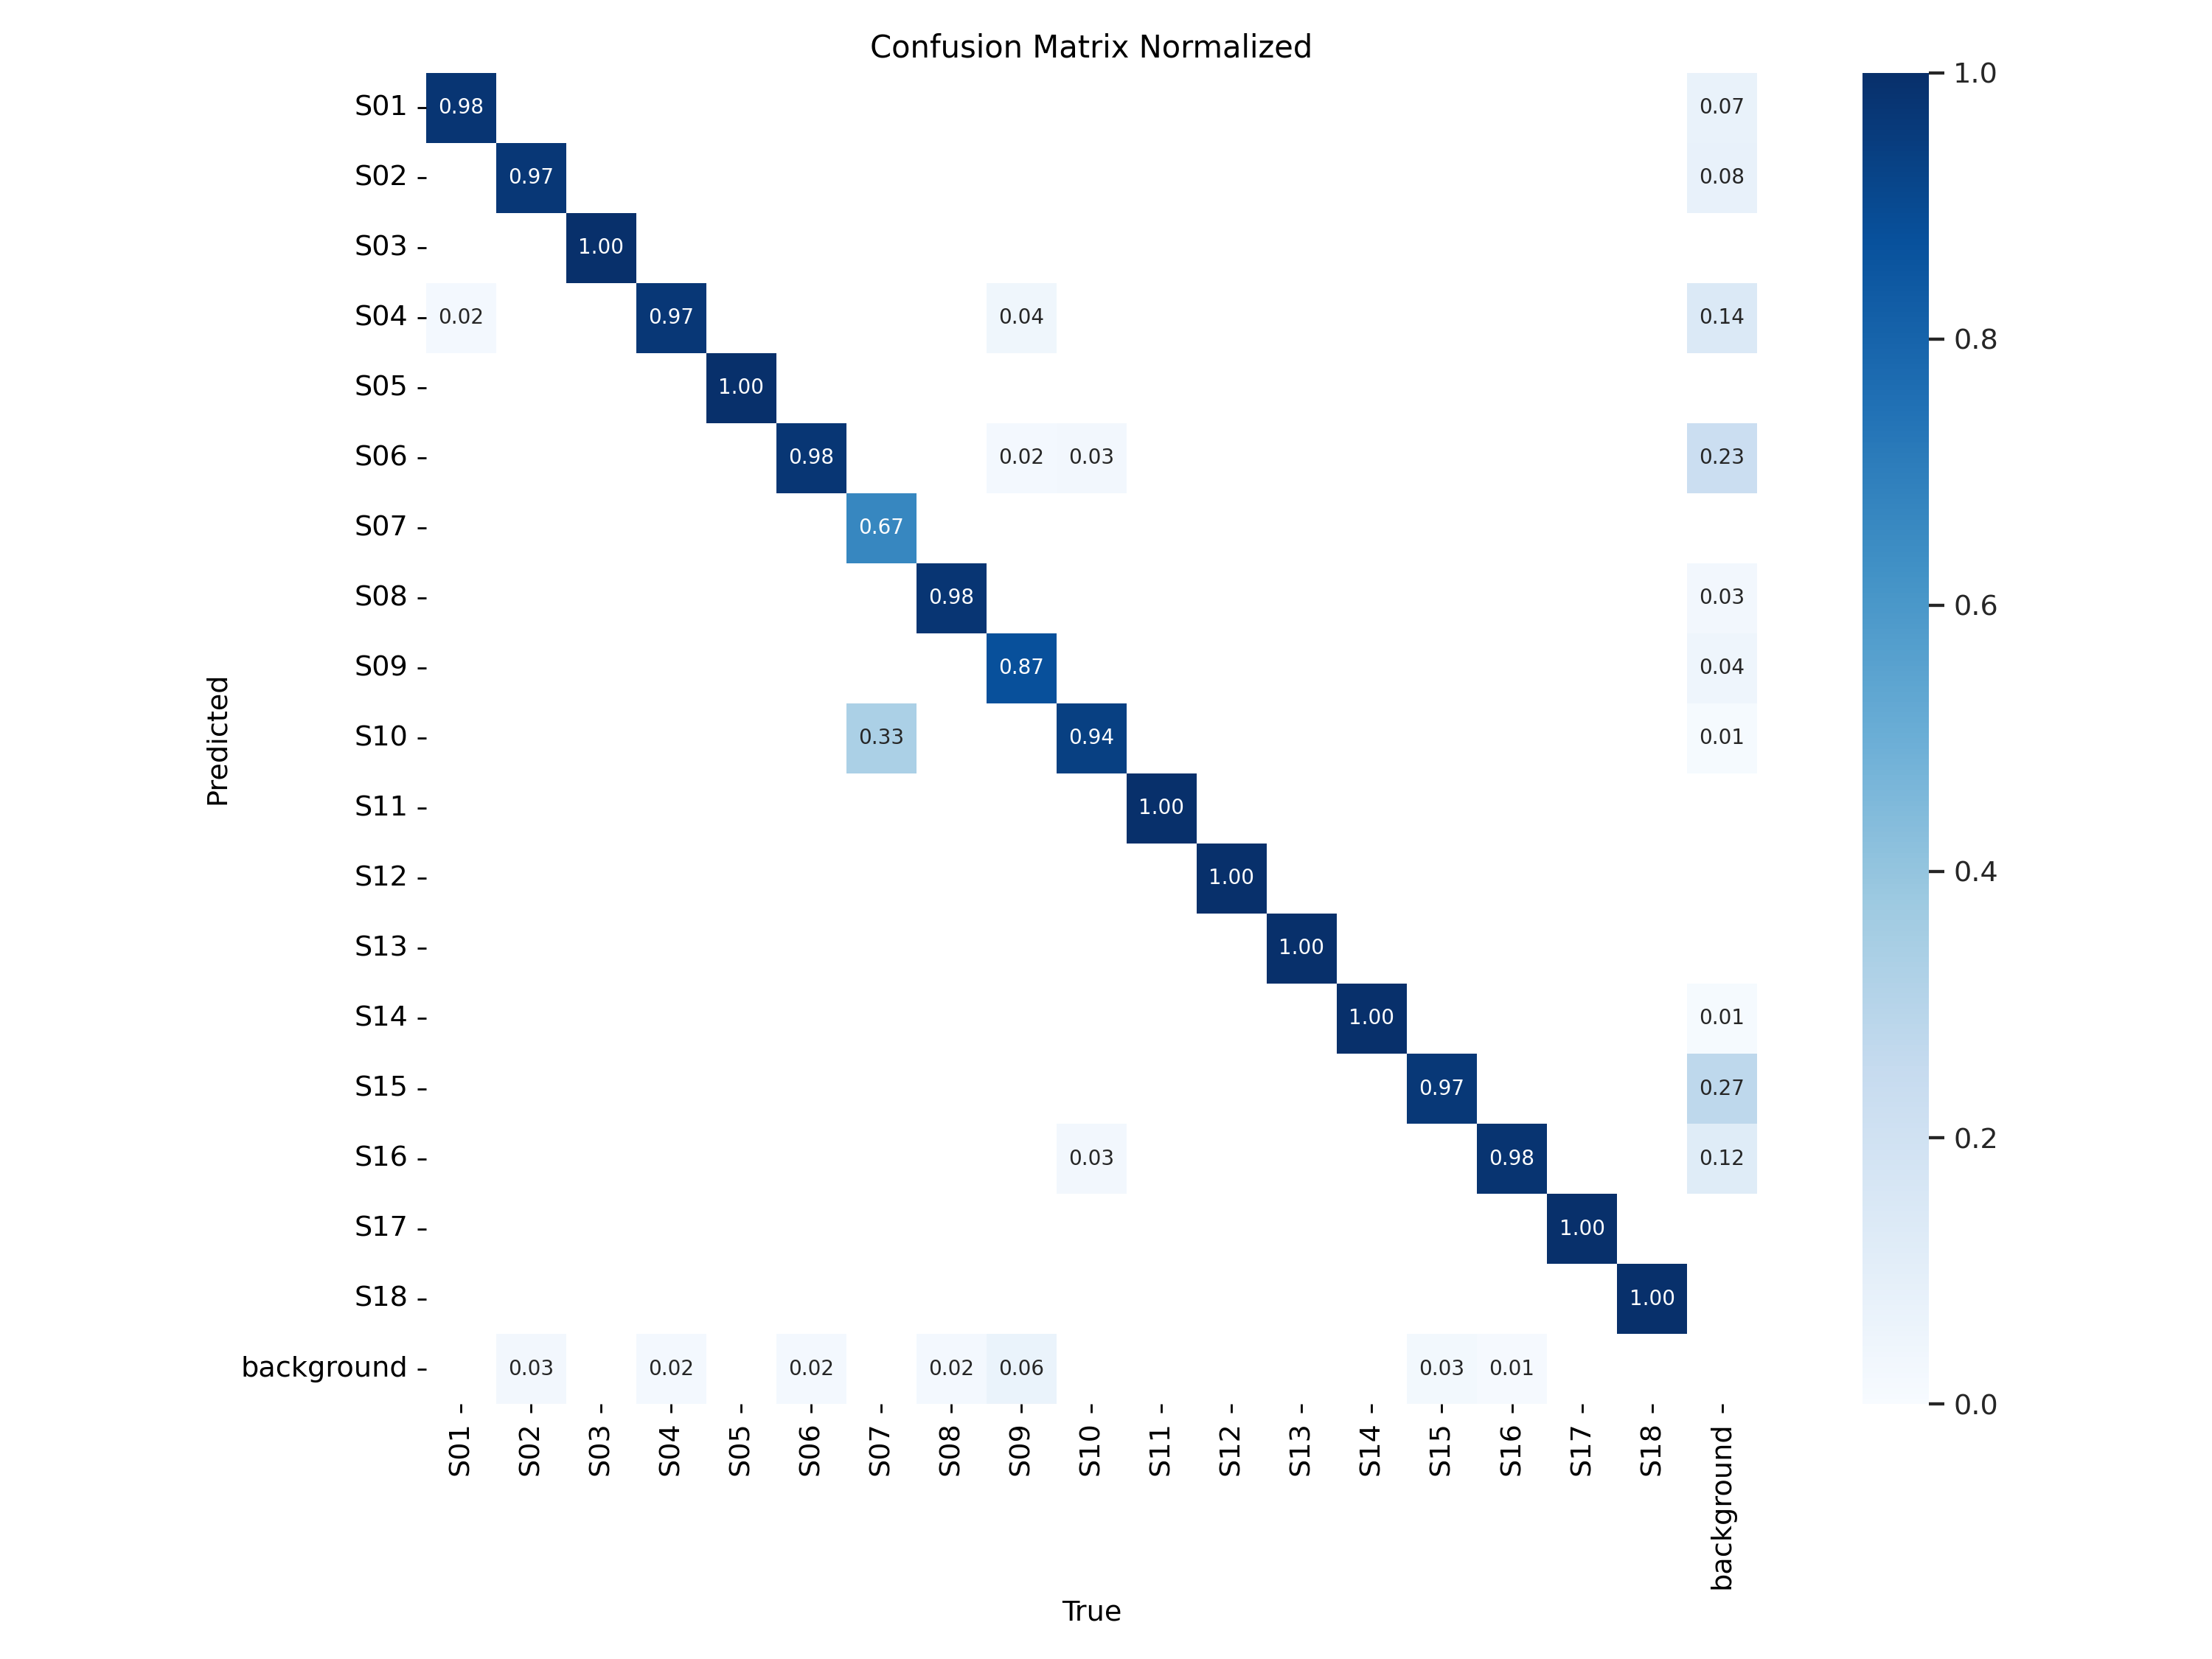
\includegraphics[width=0.85\textwidth]{figs/chap04/n_confusion_matrix_normalized.png}
    \caption{YOLOv11n混淆矩阵}
    \label{fig:nmatrix}
\end{figure}


\begin{figure}[h]
    \centering
    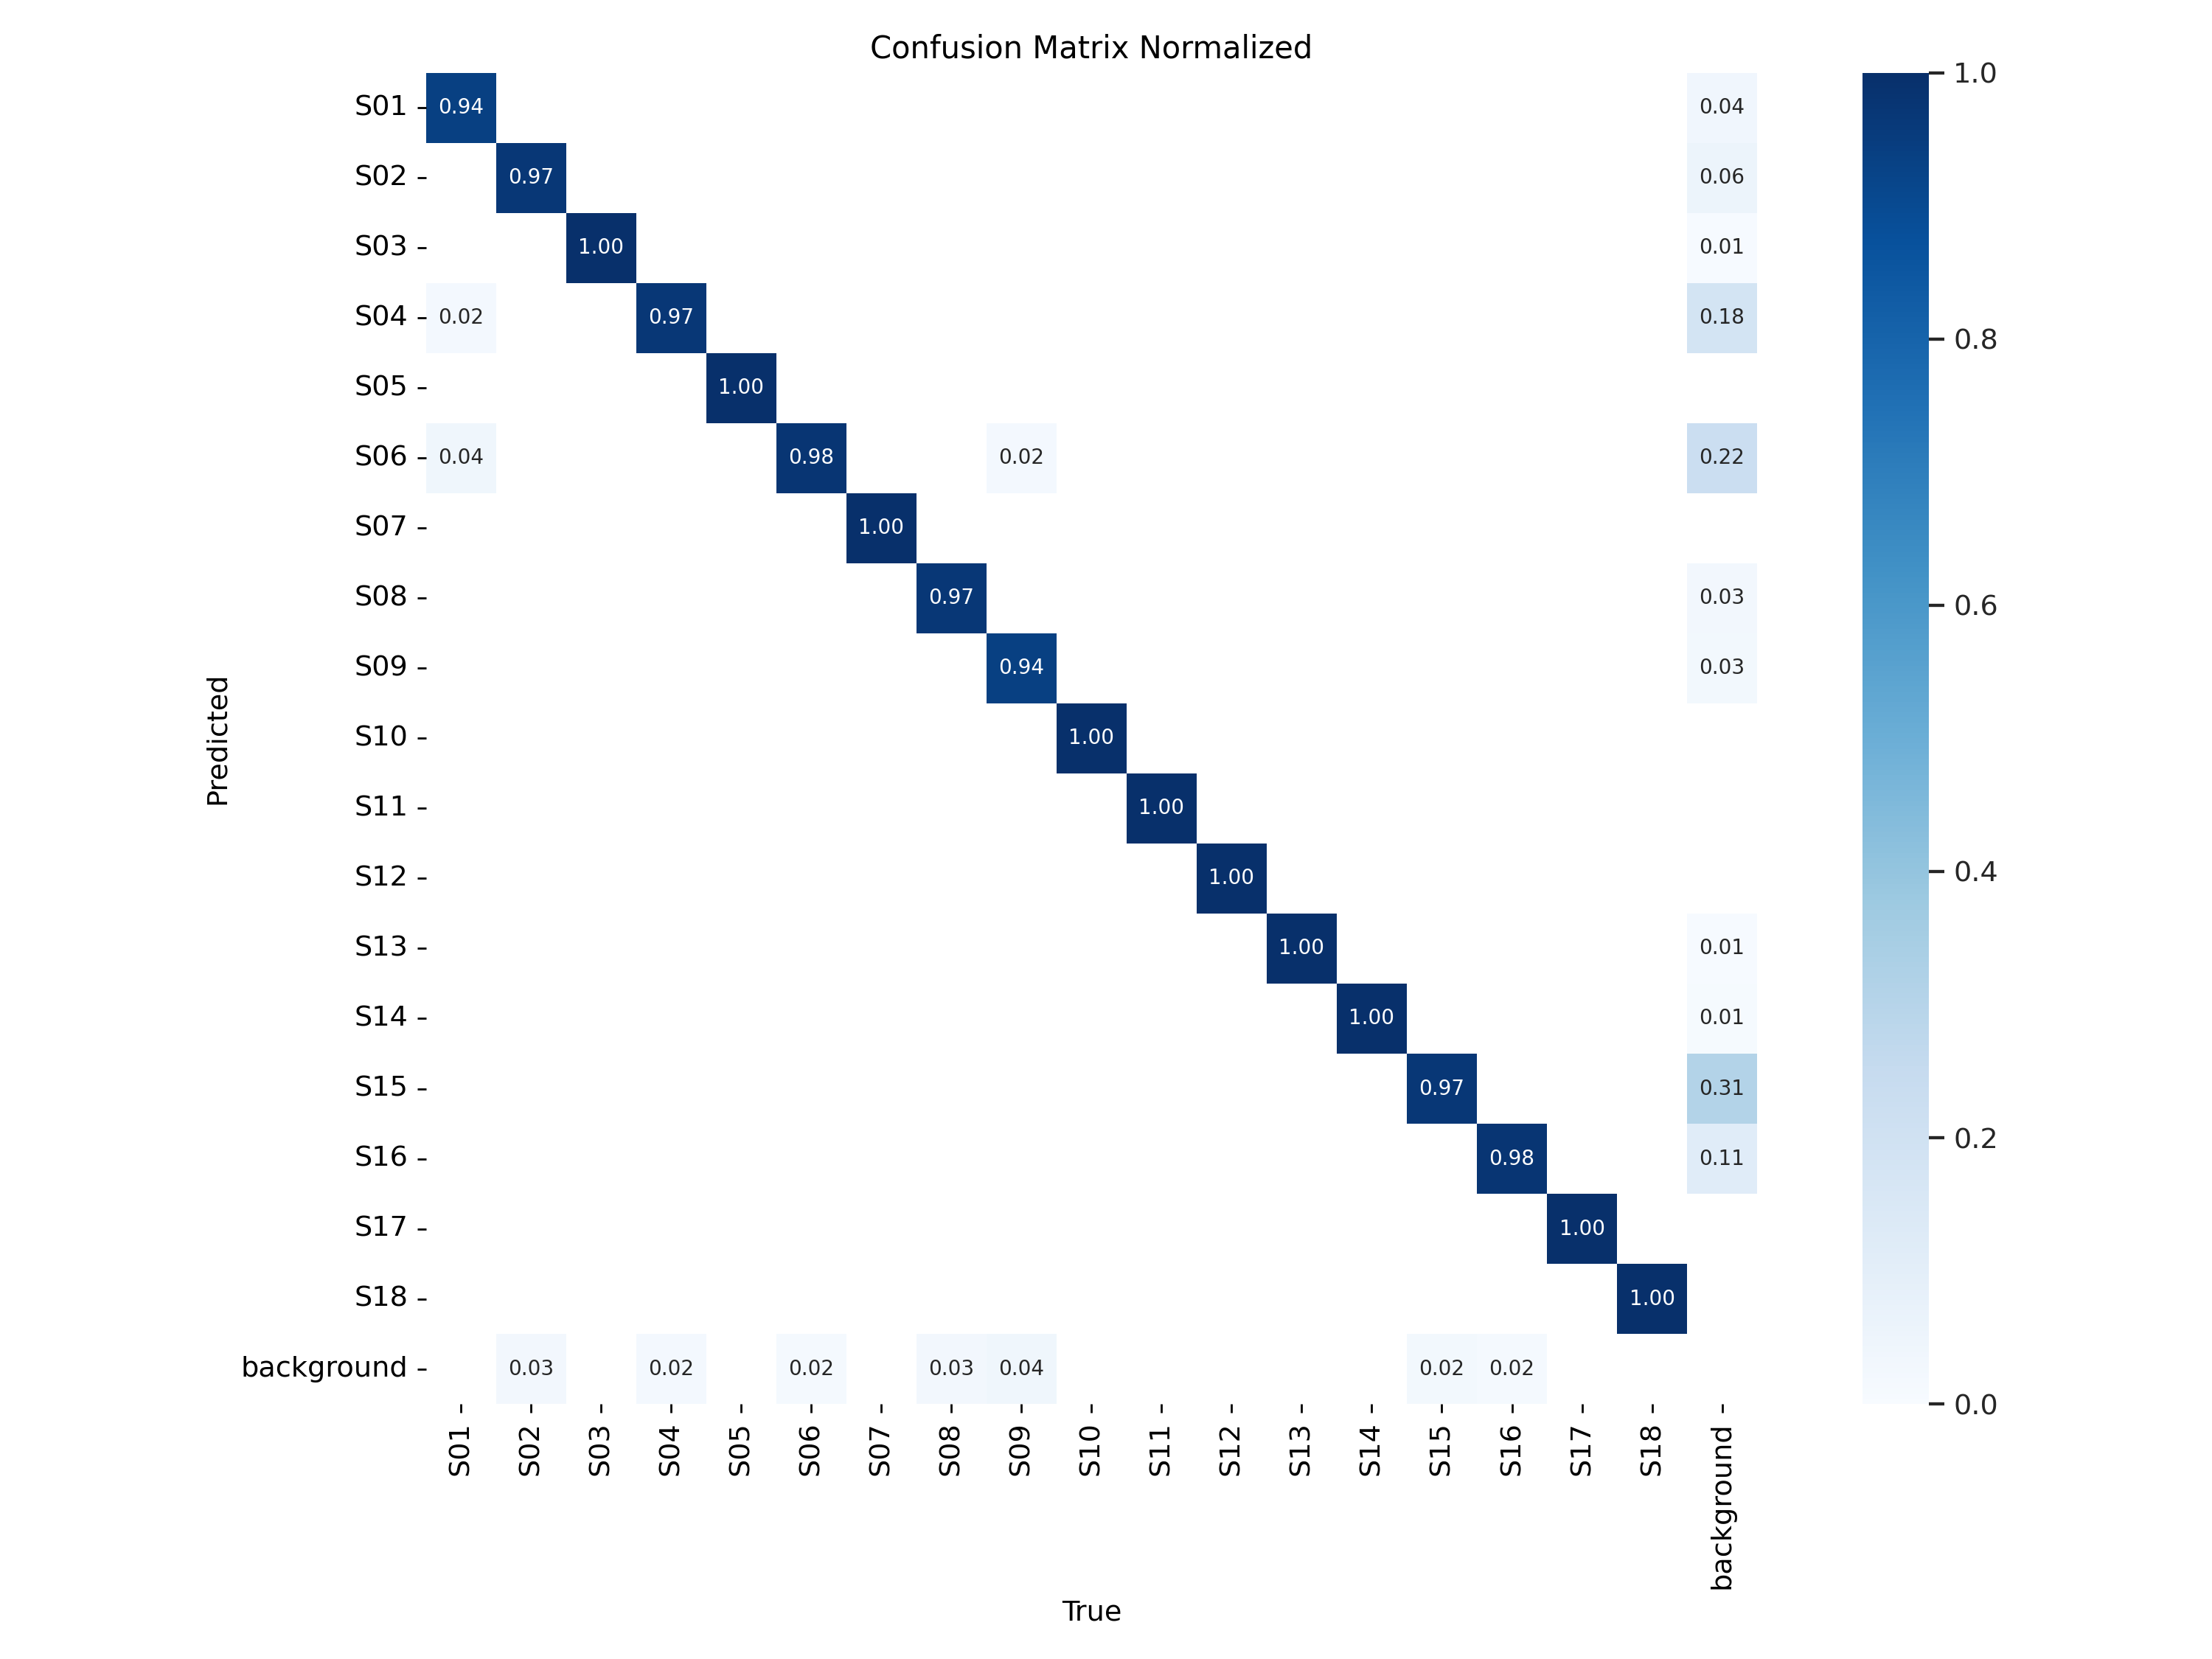
\includegraphics[width=0.85\textwidth]{figs/chap04/s_confusion_matrix_normalized.png}
    \caption{YOLOv11s混淆矩阵}
    \label{fig:smatrix}
\end{figure}


\begin{figure}[H]
    \centering
    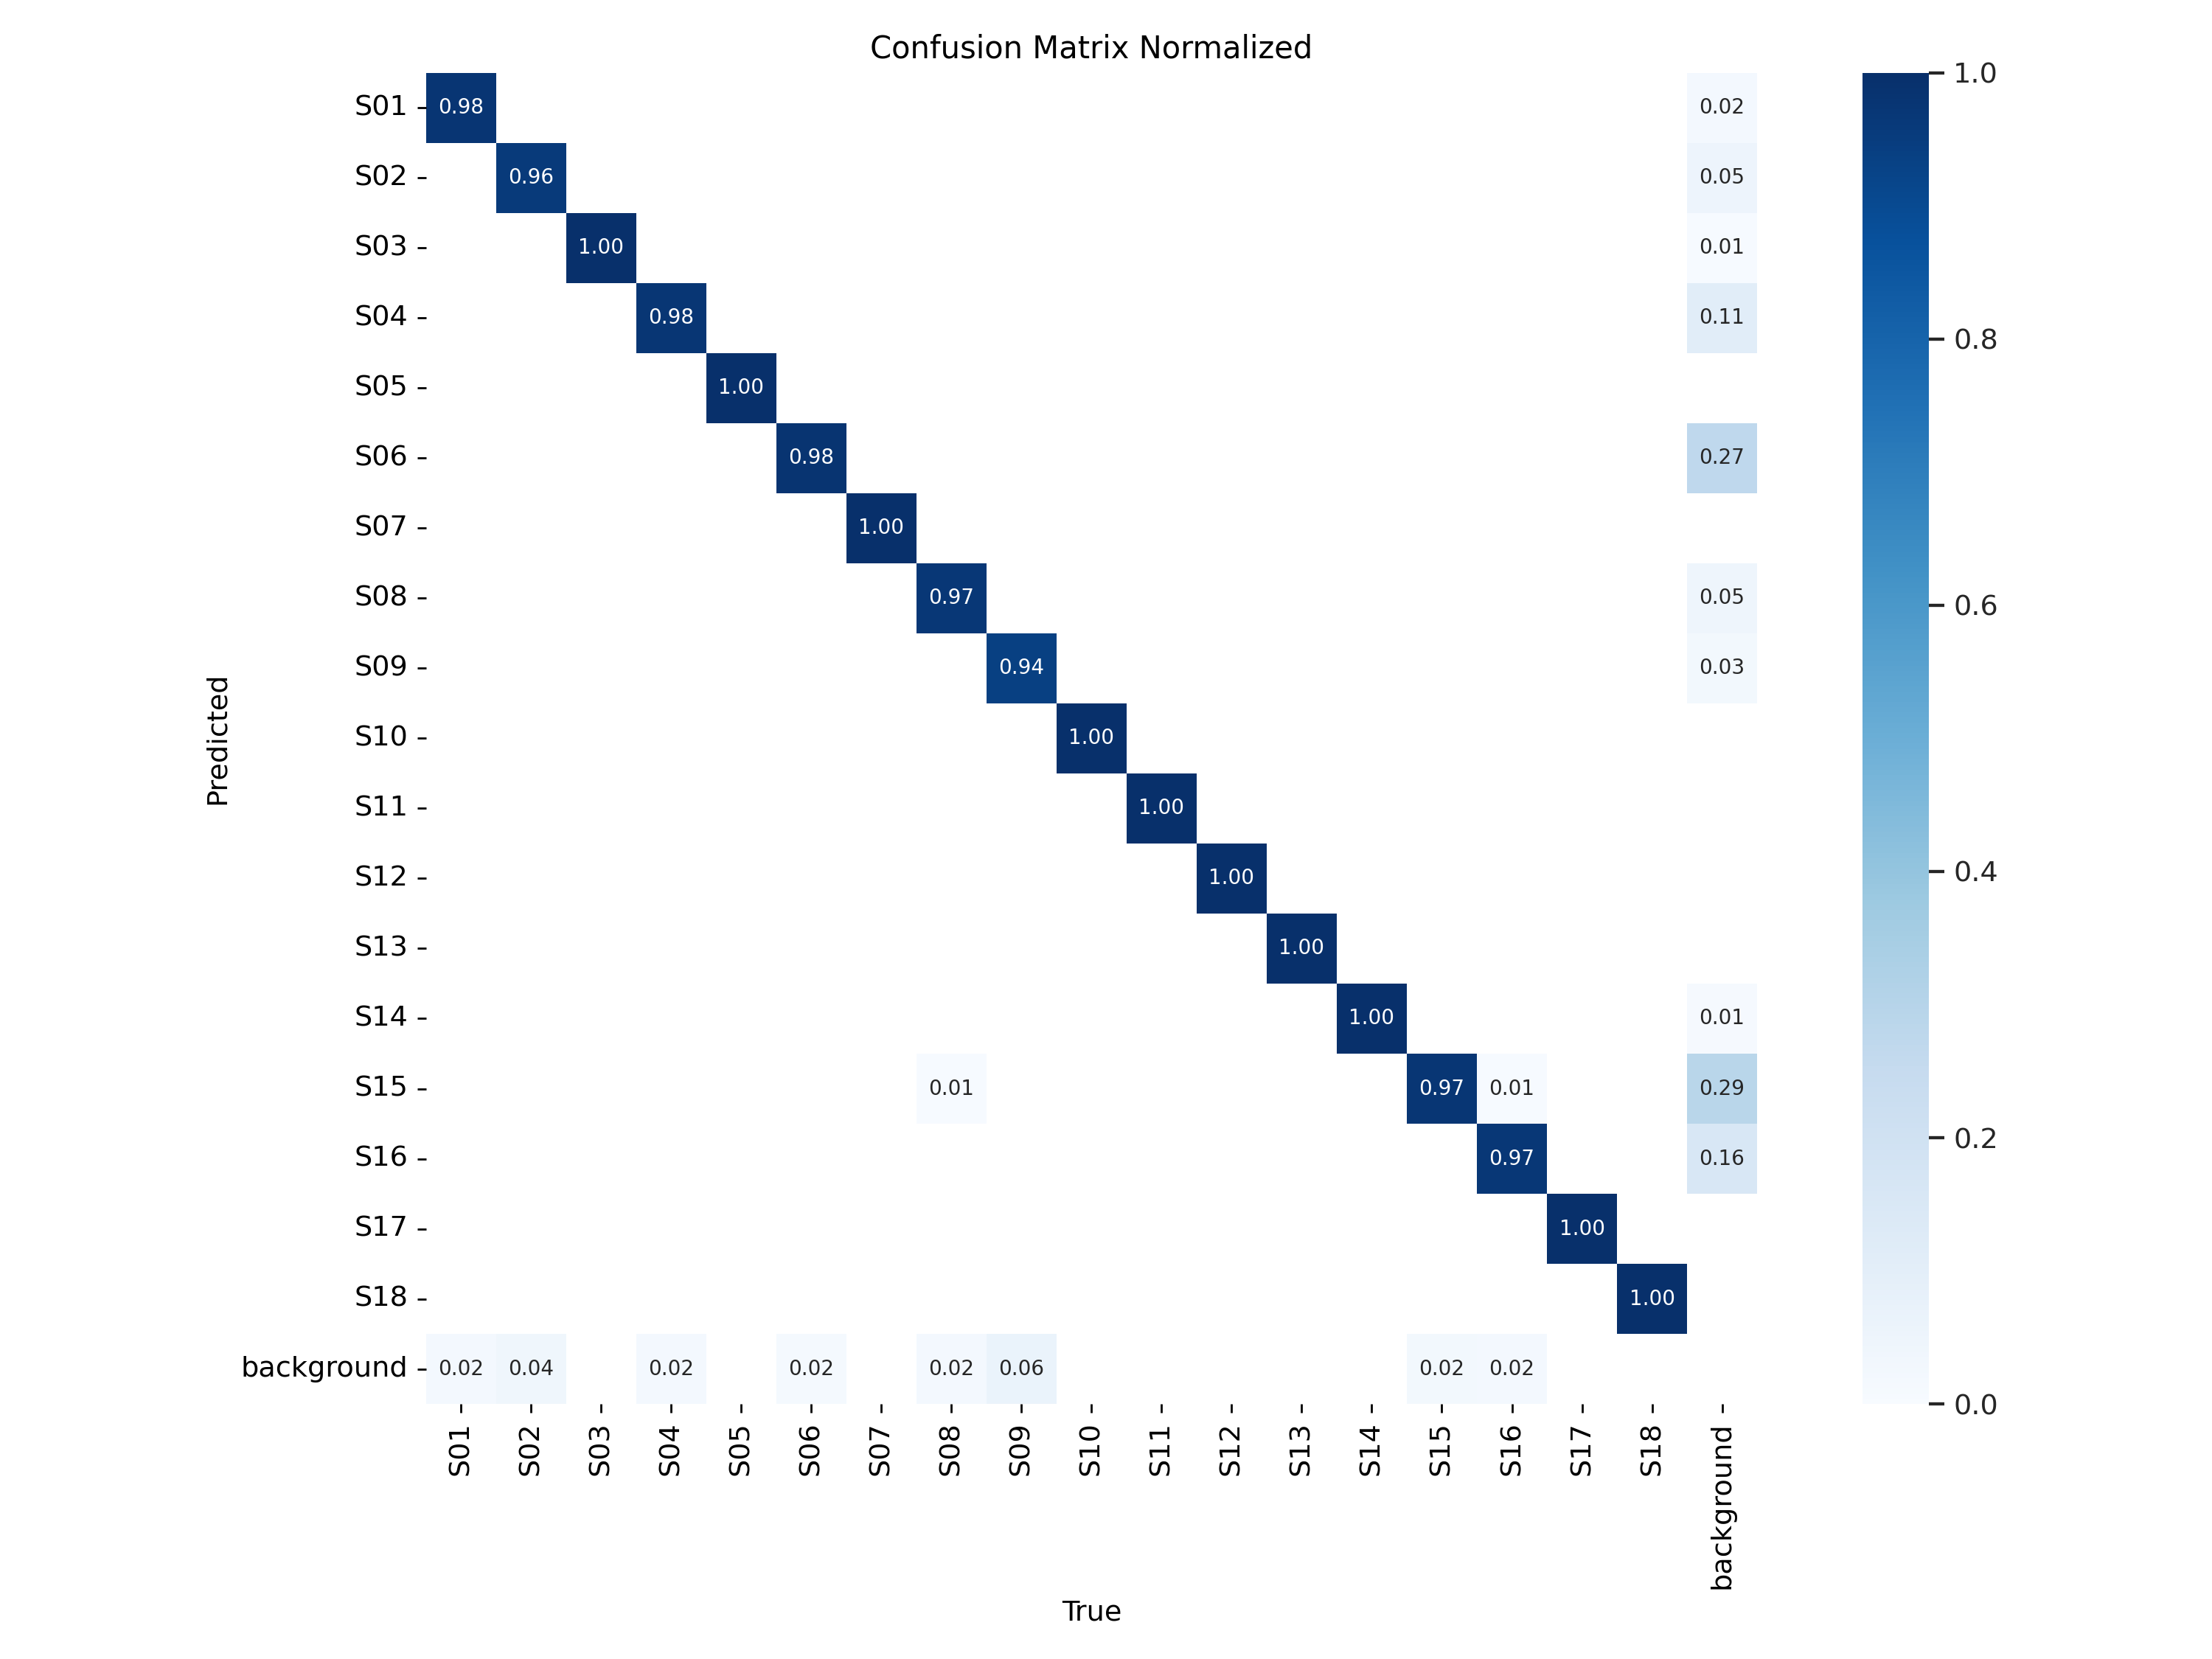
\includegraphics[width=0.85\textwidth]{figs/chap04/m_confusion_matrix_normalized.png}
    \caption{YOLOv11m混淆矩阵}
    \label{fig:mmatrix}
\end{figure}

\subsection{驾驶员id模型}
本文基于YOLOv11n、YOLOv11s和YOLOv11m三个模型,各训练了300个epoch,驾驶员id模型训练结果如\ref{fig:trackResult_part1}和\ref{fig:trackResult_part2}所示。下面同样对七个检测精度指标进行详细对比分析。

% \begin{figure}[H]
%     \centering
%     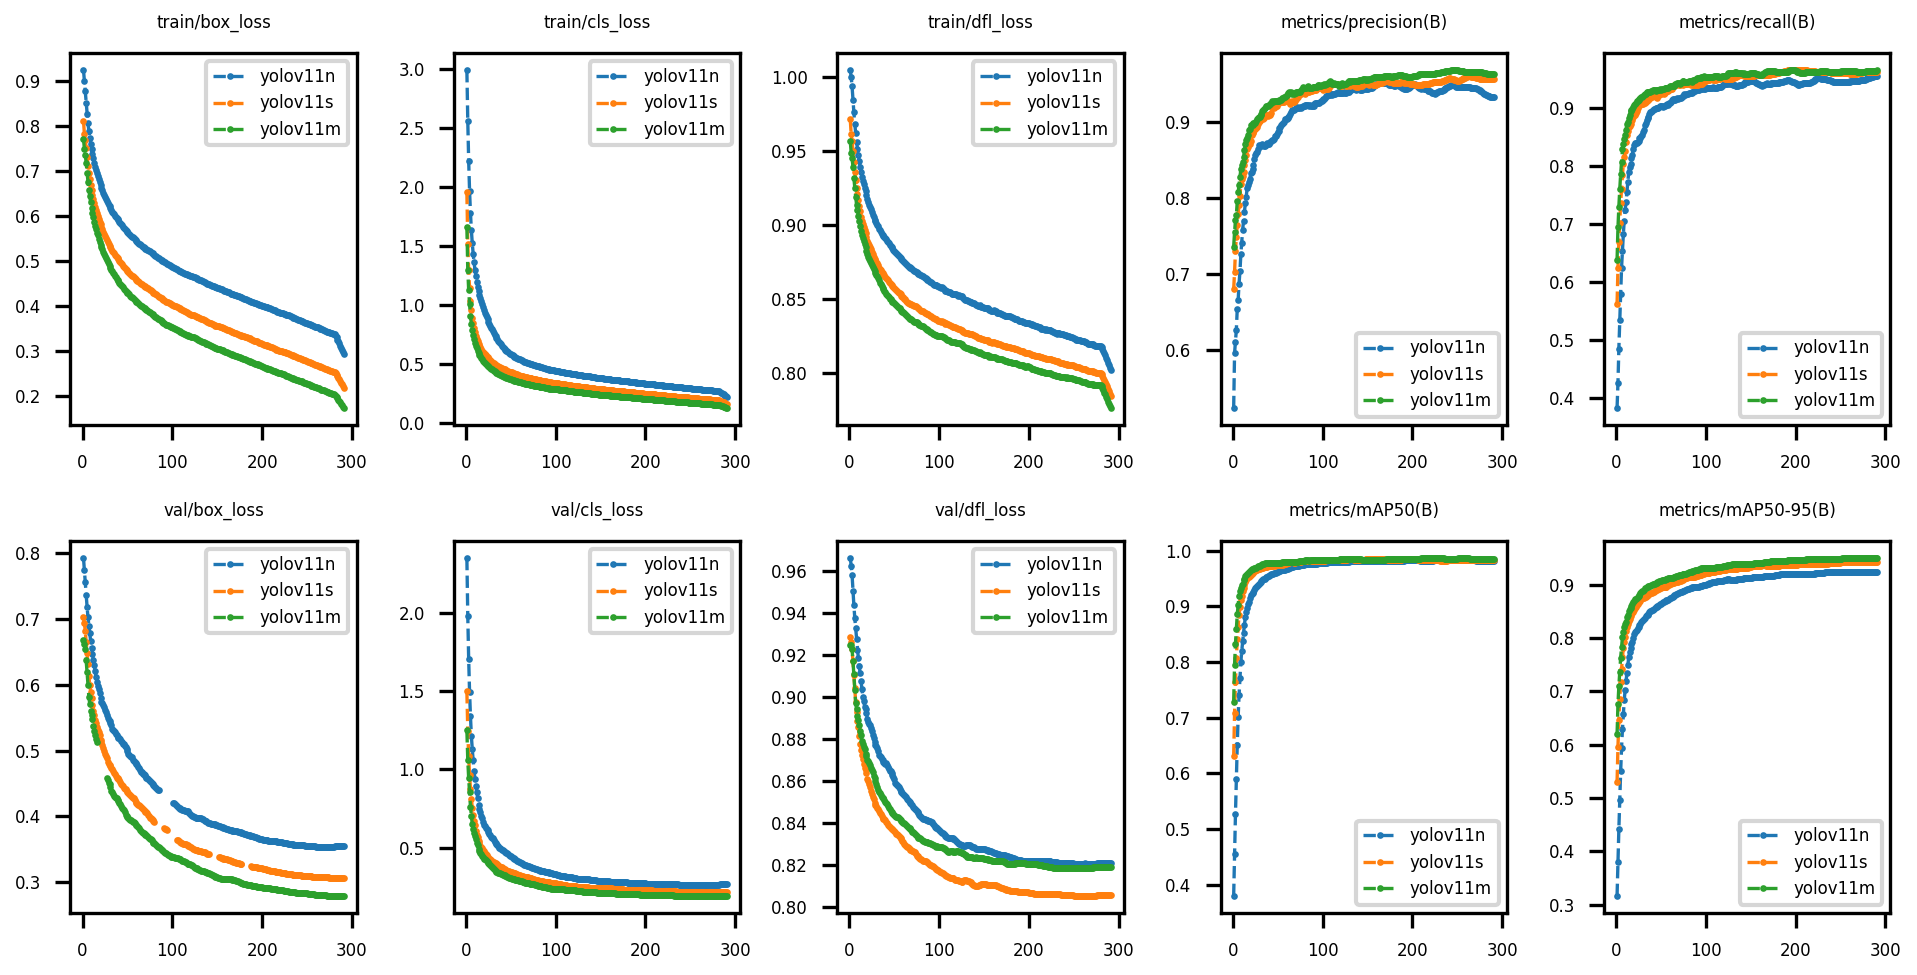
\includegraphics[width=1\textwidth]{figs/chap04/trackResult.png}
%     \caption{驾驶员id模型}
%     \label{fig:trackResult}
% \end{figure}
\begin{figure}[H]
    \centering
    \begin{subfigure}[t]{0.43\textwidth}
        \centering
        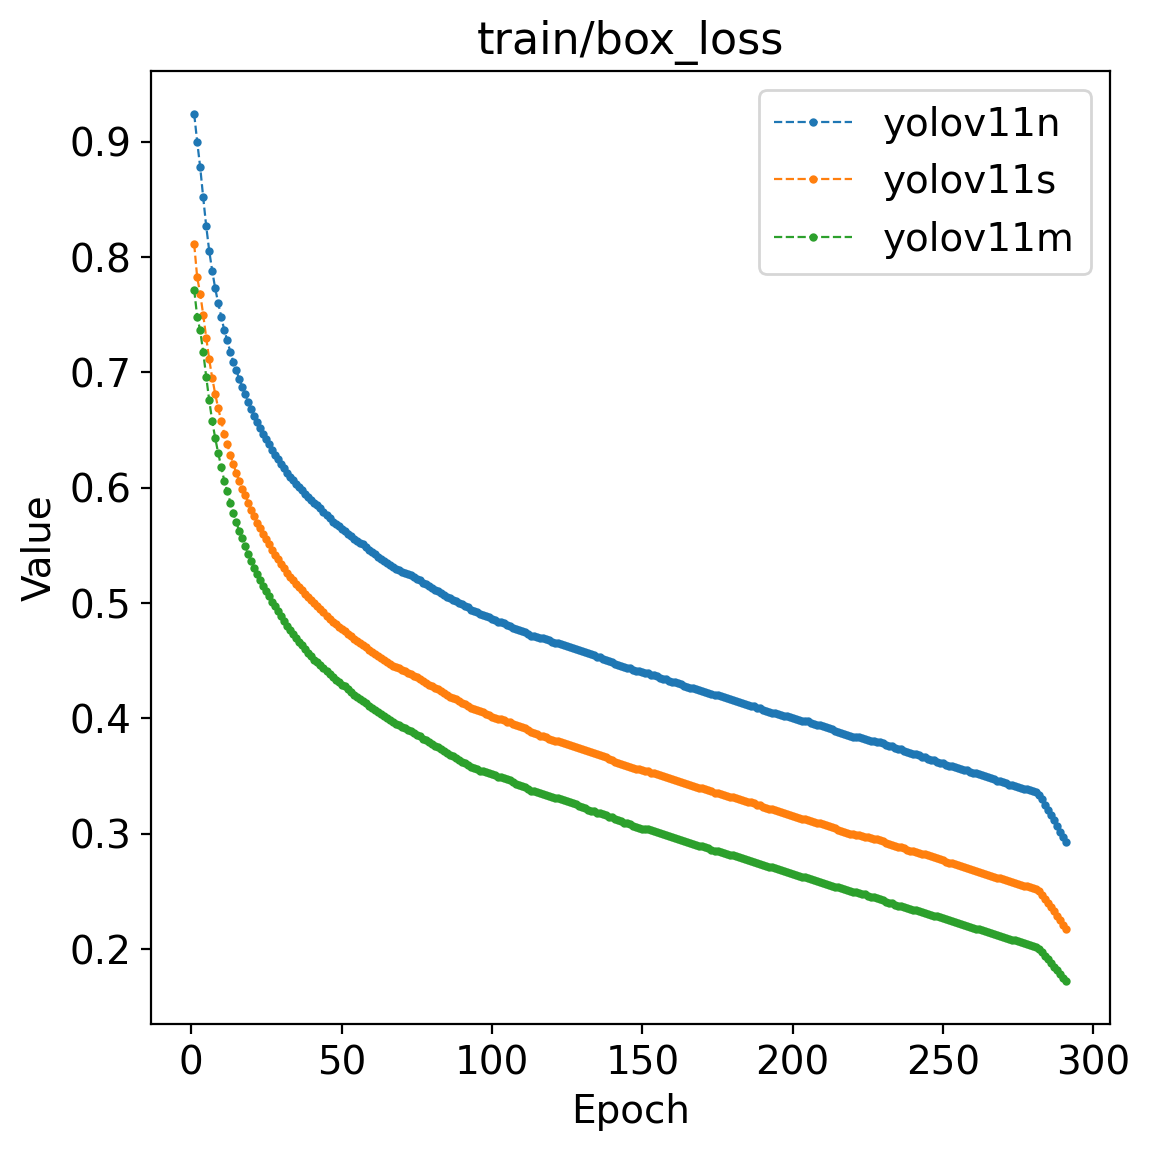
\includegraphics[width=\textwidth]{figs/chap04/track_result/track_train_box_loss.png}
        \caption{训练集边界框回归损失}
        \label{fig:track_train_box_loss}
    \end{subfigure}
    \begin{subfigure}[t]{0.43\textwidth}
        \centering
        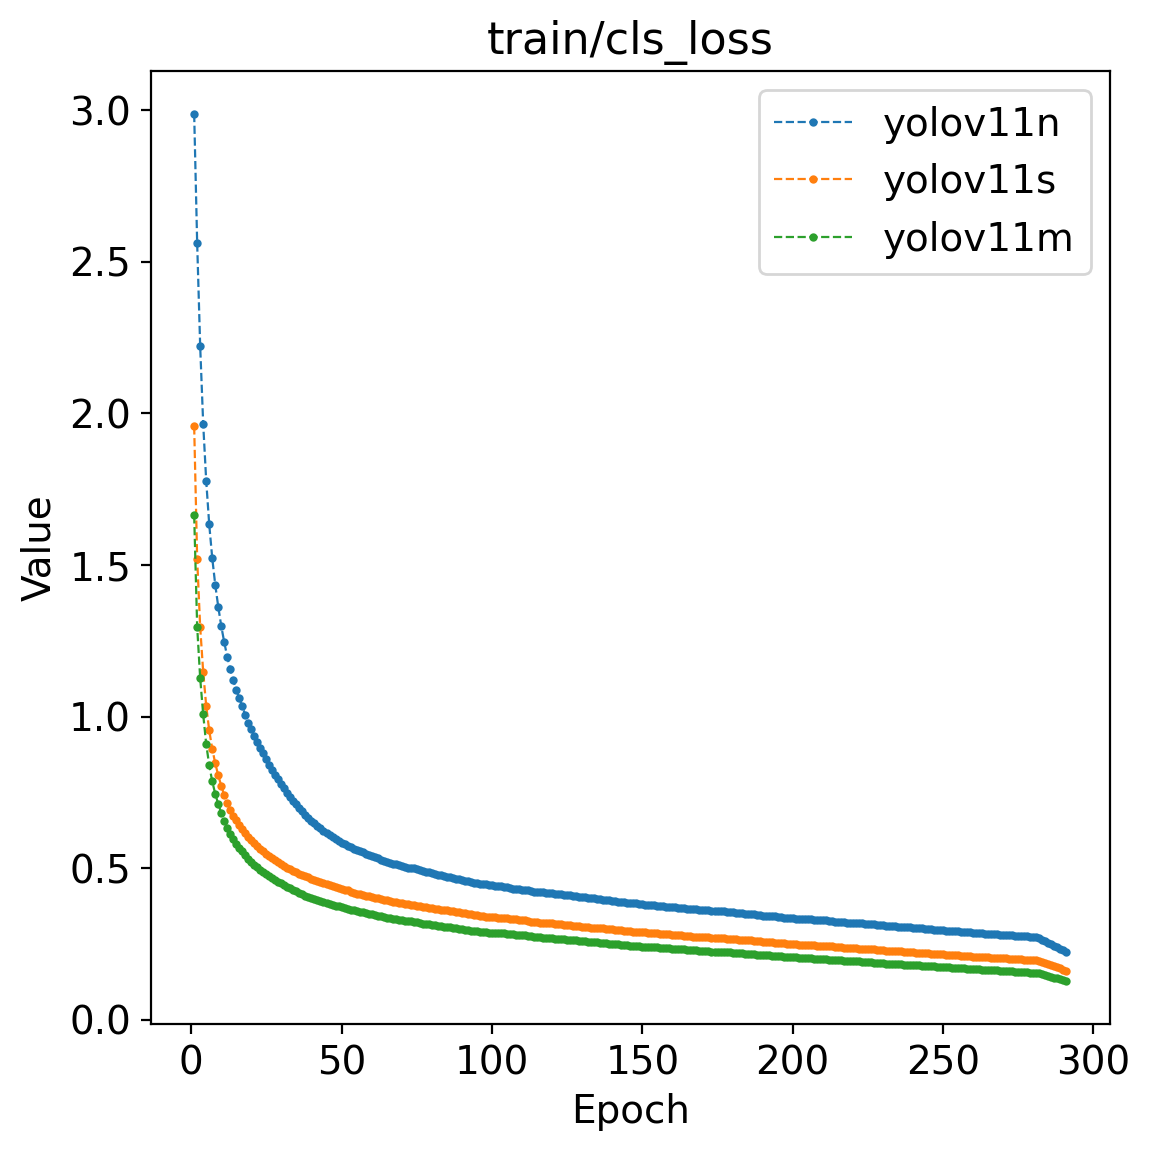
\includegraphics[width=\textwidth]{figs/chap04/track_result/track_train_cls_loss.png}
        \caption{训练集分类损失}
        \label{fig:track_train_cls_loss}
    \end{subfigure}
    \begin{subfigure}[t]{0.43\textwidth}
        \centering
        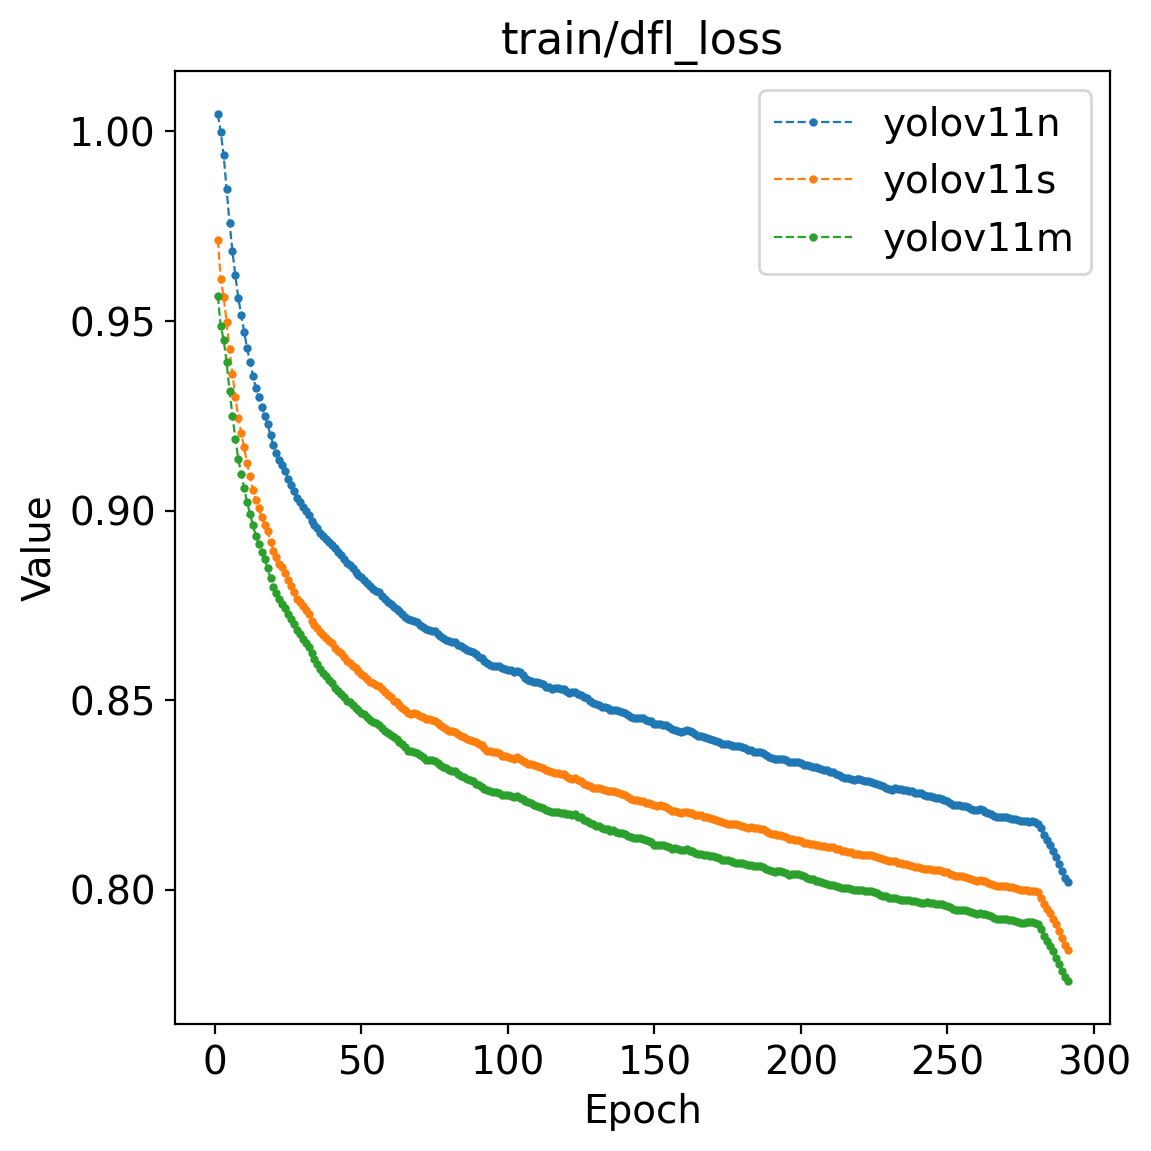
\includegraphics[width=\textwidth]{figs/chap04/track_result/track_train_dfl_loss.png}
        \caption{训练集分布损失}
        \label{fig:track_train_dfl_loss}
    \end{subfigure}
    \begin{subfigure}[t]{0.43\textwidth}
        \centering
        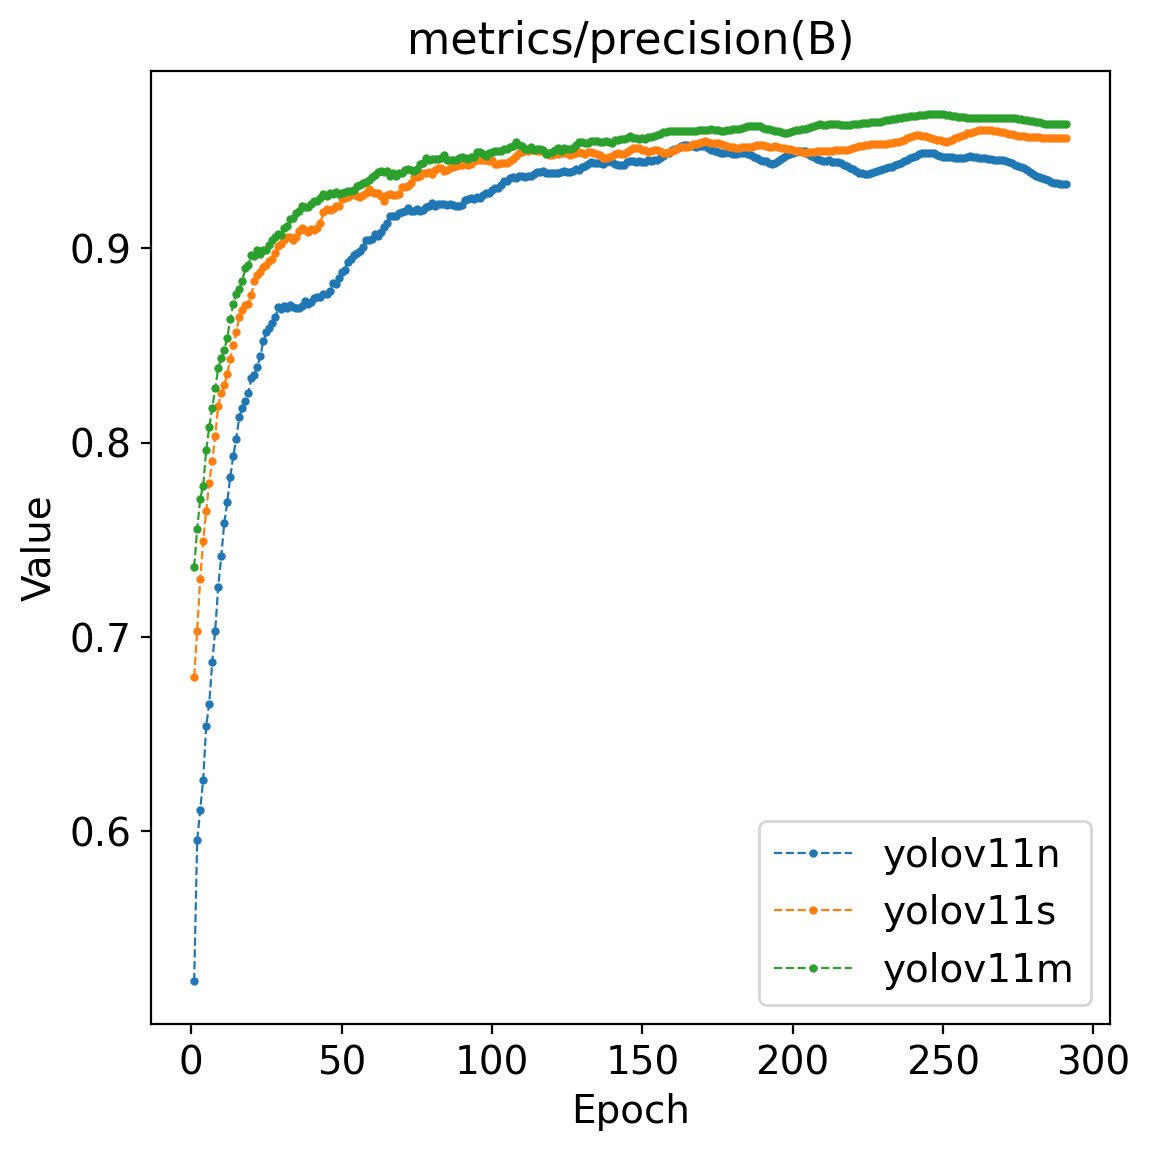
\includegraphics[width=\textwidth]{figs/chap04/track_result/track_metrics_precision(B).png}
        \caption{精度}
        \label{fig:track_metrics_precision}
    \end{subfigure}
    \caption{驾驶员id模型训练结果(第一部分)}
    \label{fig:trackResult_part1}
\end{figure}

\newpage % 这里使用 \newpage 强制分页

\begin{figure}[H]
    \centering
    \begin{subfigure}[t]{0.43\textwidth}
        \centering
        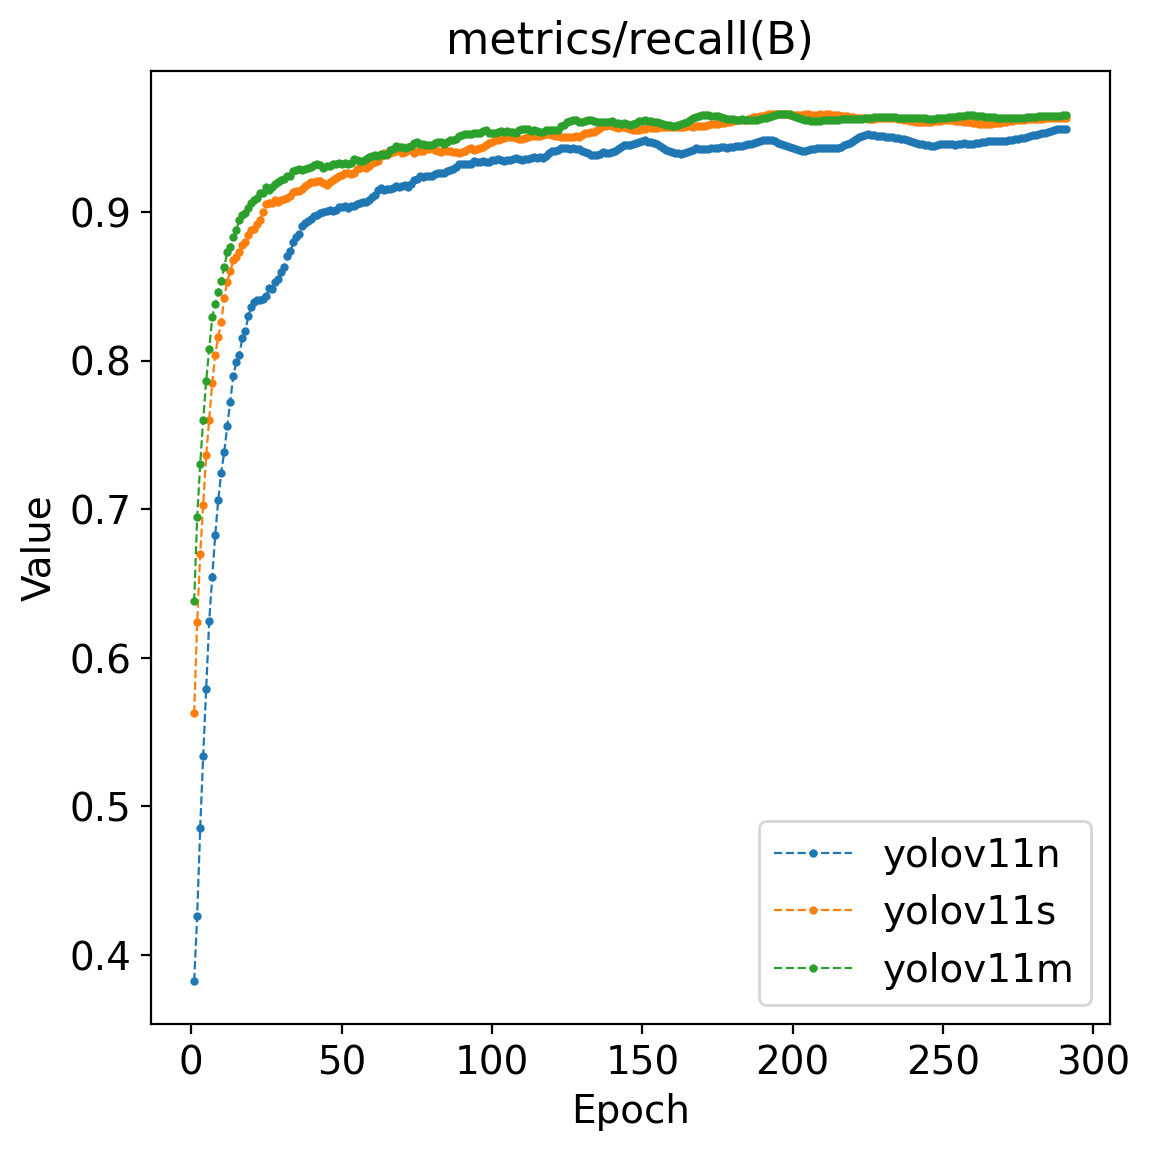
\includegraphics[width=\textwidth]{figs/chap04/track_result/track_metrics_recall(B).png}
        \caption{召回率}
        \label{fig:track_metrics_recall}
    \end{subfigure}
    \begin{subfigure}[t]{0.43\textwidth}
        \centering
        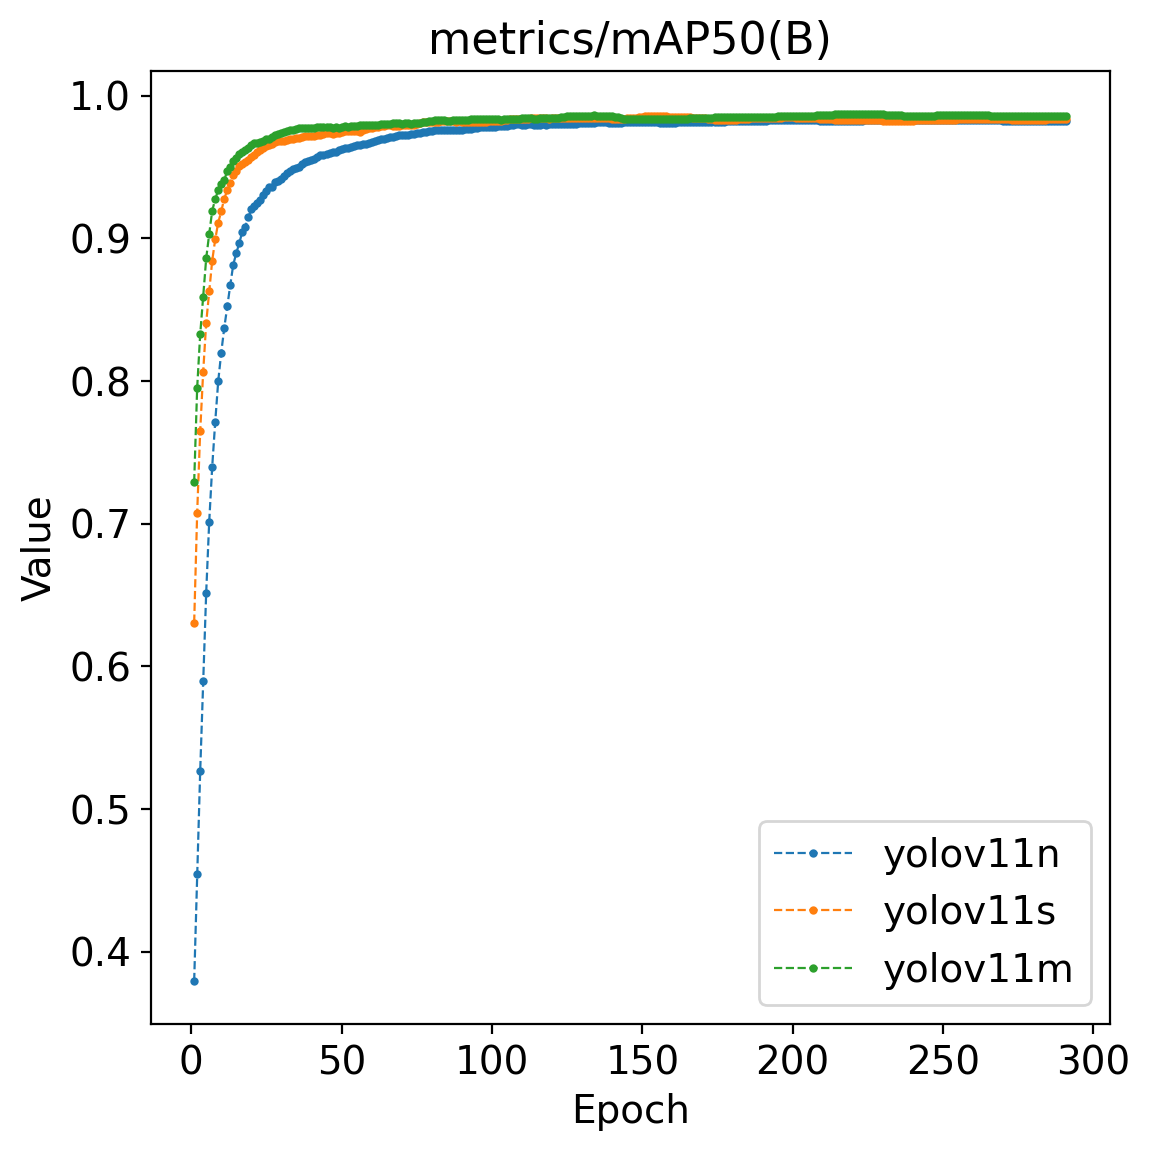
\includegraphics[width=\textwidth]{figs/chap04/track_result/track_metrics_mAP50(B).png}
        \caption{mAP50}
        \label{fig:track_metrics_mAP50}
    \end{subfigure}
    \begin{subfigure}[t]{0.43\textwidth}
        \centering
        \includegraphics[width=\textwidth]{figs/chap04/track_result/track_metrics_mAP50-95(B).png}
        \caption{mAP50-95}
        \label{fig:track_metrics_mAP50-95}
    \end{subfigure}
    \begin{subfigure}[t]{0.43\textwidth}
        \centering
        \includegraphics[width=\textwidth]{figs/chap04/track_result/track_val_box_loss.png}
        \caption{验证集边界框回归损失}
        \label{fig:track_val_box_loss}
    \end{subfigure}
    \begin{subfigure}[t]{0.43\textwidth}
        \centering
        \includegraphics[width=\textwidth]{figs/chap04/track_result/track_val_cls_loss.png}
        \caption{验证集分类损失}
        \label{fig:track_val_cls_loss}
    \end{subfigure}
    \begin{subfigure}[t]{0.43\textwidth}
        \centering
        \includegraphics[width=\textwidth]{figs/chap04/track_result/track_val_dfl_loss.png}
        \caption{验证集分布损失}
        \label{fig:track_val_dfl_loss}
    \end{subfigure}
    \caption{驾驶员id模型训练结果(第二部分)}
    \label{fig:trackResult_part2}
\end{figure}

边界框回归损失:YOLOv11s和YOLOv11m两个模型的边界框回归损失在前期下降速度相较于YOLOv11n略快,中期以后三者下降速度相近。YOLOv11m训练得到的边界框回归损失最优,数值最小,YOLOv11s次之,YOLOv11n相对较高。说明YOLOv11m模型预测驾驶员id的边界框更精确。

分类损失:YOLOv11s和YOLOv11m的分类损失在前期下降较快,YOLOv11n稍慢一些,中期以后三者下降速度近似。YOLOv11m的分类损失值最小,其次是YOLOv11s,YOLOv11n的值最高。YOLOv11m模型对驾驶员id的分类效果更好。

分布损失:YOLOv11m和YOLOv11s的分类损失值收敛较快,YOLOv11n收敛相对较慢。训练结束时YOLOv11m的分布损失值最小,效果最好,YOLOv11s次之,YOLOv11n的值最大。

精度:YOLOv11m收敛速度最快,最早到达较高水平并趋于平稳。YOLOv11n和YOLOv11s上升速度相对较慢。最终YOLOv11m达到的精度最高,其次是YOLOv11s,YOLOv11n的精度最低。这表明YOLOv11m对驾驶员id的预测更准确。

召回率:YOLOv11m和YOLOv11s的收敛趋势近似,且都比YOLOv11n的收敛速度要快。YOLOv11m和YOLOv11s最终的召回率相近,都比YOLOv11n的召回率要高。说明YOLOv11m和YOLOv11n能找到更多的正例驾驶员id目标。

mAP50:YOLOv11m和YOLOv11s的mAP50值收敛趋势比较相似,都比YOLOv11n的收敛速度要快。最终三个模型的mAP50值几乎相同。

mAP50-95:YOLOv11m的mAP50-95值收敛速度最快,其次是YOLOv11s,YOLOv11n的收敛速度最慢。训练结束时,YOLOv11m达到了最高的mAP50-95值;YOLOv11s次之;YOLOv11n相对较低。

将上述七个指标训练过程中的最优值进行对比如\ref{tab:modelCompare2}。三个损失函数(box\_loss、cls\_loss、dfl\_loss)随模型规模增大,最优值不断减小;四个精度指标(precision、recall、mAP50、mAP50-95)则随模型规模增大,最优值持续升高,模型检测精度随之提升。

\begin{table}[htb]
    \centering
    \caption[指标对比]{模型损失函数与检测精度指标对比2\label{tab:modelCompare2}}
    \begin{tabular}{lccccccc}
        \toprule
        Model & 
        \makecell{box\_loss\\(\%)} & 
        \makecell{cls\_loss\\(\%)} & 
        \makecell{dfl\_loss\\(\%)} & 
        \makecell{Precision\\(\%)} & 
        \makecell{Recall\\(\%)} & 
        \makecell{mAP50\\(\%)} & 
        \makecell{mAP50-95\\(\%)} \\
        \midrule
        YOLOv11n & 28.5 & 21.9 & 79.9 & 95.6 & 95.8 & 98.3 & 92.5 \\
        YOLOv11s & 21.0 & 15.7 & 78.2 & 96.1 & 96.7 & 98.7 & 94.3 \\
        YOLOv11m & 16.6 & 12.4 & 77.3 & 96.9 & 96.9 & 98.7 & 95.0 \\
        \bottomrule
    \end{tabular}
\end{table}

三个模型的检测速度对比如\ref{tab:speedCompare2}。随着模型规模增大,每秒处理帧数降低,实时性变差;且FLOPs数值增大,说明在预测中进行的浮点运算次数更多,理论上需要更长的推理时间。

\begin{table}[htb]
    \centering
    \caption[目标数据]{模型检测速度对比2\label{tab:speedCompare2}}
    \begin{tabular}{lcc}
        \toprule
        Model & 
        \makecell{FPS(1)} & 
        \makecell{FLOPs(G)} \\
        \midrule
        YOLOv11n & 67.11 & 7.49 \\
        YOLOv11s & 66.67 & 22.68 \\
        YOLOv11m & 55.87 & 70.45 \\
        \bottomrule
    \end{tabular}
\end{table}

综合上述对比结果,YOLOv11n在检测驾驶员id场景下检测精度较低,但是检测速度最快,计算复杂度最低,适合对精度要求不是很高的实时检测场景;YOLOv11s的检测精度和速度更加平衡,适合对精度和速度都有一定要求的场景;YOLOv11m有着最高的检测精度,但带来的资源开销更大,适合高精度检测场景。

\section{本章小结}
本章首先介绍了目标检测模型检测精度和检测速度的几个重要评价指标,然后对本文进行的两个模型训练结果进行展示,对YOLOv11n、YOLOv11s和YOLOv11m三个模型的检测精度与检测速度进行了对比分析。YOLOv11系列不同规模的模型具有不同的性能特征与适用场景:YOLOv11n以牺牲部分检测精度为代价,换取了卓越的检测速度,特别适用于对实时性要求严苛的场景,如智能监控、自动驾驶的实时感知模块;YOLOv11s在检测精度与速度之间取得了良好的平衡,能够满足多数场景下对二者的综合需求,是通用目标检测任务的优选方案;YOLOv11m则有着更高的检测精度,尽管检测速度相对较慢,却在对精度要求极高的复杂场景中展现出显著优势,例如工业缺陷检测、医疗影像分析等对准确性要求苛刻的领域。

% \subsection{YOLOv11n}
% 本文基于YOLOv11n训练了300个epoch,训练结果如\ref{fig:nresult}所示。从实验结果可知,模型的最高精度为96.7\%,最高召回率为96.6\%,mAP50为99.0\%,mAP50-95为94.1\%。
% \begin{figure}[H]
%     \centering
%     \includegraphics[width=0.8\textwidth]{figs/chap04/n_results.png}
%     \caption{YOLOv11n训练结果}
%     \label{fig:nresult}
% \end{figure}

% 基于YOLOv11n训练出的模型的混淆矩阵见\ref{fig:nmatrix},模型对大部分目标的分类效果都不错,18个标签中有15个标签的判断准确率达到了97\%。对S07这一类别的分类效果较差,对其中33\%的数据都预测为了S10,仅有67\%的正确率。该模型的P-R曲线见\ref{fig:npr},可以看出mAP@0.5为99.0\%。



% \begin{figure}[H]
%     \centering
%     \includegraphics[width=0.6\textwidth]{figs/chap04/n_PR_curve.png}
%     \caption{YOLOv11nP-R曲线}
%     \label{fig:npr}
% \end{figure}

% \subsection{YOLOv11s}
% 本文基于YOLOv11s训练了300个epoch,训练结果见\ref{fig:sresult}。该模型的最高精度为96.2\%,最高召回率为97.2\%,mAP50为99.0\%,mAP50-95为95.4\%。

% \begin{figure}[H]
%     \centering
%     \includegraphics[width=0.8\textwidth]{figs/chap04/s_results.png}
%     \caption{YOLOv11s训练结果}
%     \label{fig:sresult}
% \end{figure}

% \ref{fig:smatrix}展示了该模型的混淆矩阵,可以看出模型对S01类别有6\%的误判,其中2\%预测为了S04,4\%预测为了S06。对S09类别有2\%的误判,预测成了S06,以及4\%的漏判,其他的类别的准确率都达到了97\%。YOLOv11s训练结果的P-R曲线如\ref{fig:spr},该模型的mAP@0.5为99.0\%。




% \begin{figure}[H]
%     \centering
%     \includegraphics[width=0.6\textwidth]{figs/chap04/s_PR_curve.png}
%     \caption{YOLOv11sP-R曲线}
%     \label{fig:spr}
% \end{figure}

% \subsection{YOLOv11m}
% 本文基于YOLOv11m训练了300个epoch,实验结果如\ref{fig:mresult}所示,该模型的最高精度为97.3\%,最高召回率为98.1\%,mAP50为99.1\%,mAP50-95为95.5\%。

% \begin{figure}[H]
%     \centering
%     \includegraphics[width=0.8\textwidth]{figs/chap04/m_results.png}
%     \caption{YOLOv11m训练结果}
%     \label{fig:mresult}
% \end{figure}

% 混淆矩阵如\ref{fig:mmatrix}所示,模型对S04类别有4\%的漏判,对S9类别有6\%的漏判,其他类别的准确率都达到了97\%。P-R曲线为\ref{fig:mpr},该模型的mAP@0.5为99.1\%。

% \begin{figure}[H]
%     \centering
%     \includegraphics[width=0.6\textwidth]{figs/chap04/m_PR_curve.png}
%     \caption{YOLOv11mP-R曲线}
%     \label{fig:mpr}
% \end{figure}

% \subsection{模型性能对比}
% 本文基于YOLOv11三种不同的模型对摩托车驾乘人员头盔佩戴数据集进行了训练,\ref{tab:modelCompare}展示了各个模型在精度、召回率、mAP50、mAP50-95以及检测速度这五个方面的对比。

% 三个模型的精度均在96\% 以上。其中,YOLOv11m的精度最高,为97.3\%。三个模型的召回率也都处于较高水平,都在96\%以上。YOLOv11m的召回率最高,为98.1\%。三个模型的mAP50值几乎一致,都在99\%附近,最大仅相差0.1\%,说明在IoU阈值为0.5时,它们对目标物体的检测效果都非常好。在mAP50-95指标上,YOLOv11m和YOLOv11s表现较好,分别为95.5\%和95.4\%,仅相差0.1\%,都要高于YOLOv11n的94.1\%,这表明在更严格的IoU阈值范围内,YOLOv11m和YOLOv11s 的性能更优。

% 在检测速度方面,平均检测一张图片YOLOv11m耗时最长,为31.5ms,YOLOv11s为27.3ms,比YOLOv11m快了13.3\%。YOLOv11n最快,为24ms,比YOLOv11s快了12.1\%,比YOLOv11m快了23.8\%。

% 根据分析可知,YOLOv11n在速度上具有明显优势,适用于对实时性要求较高的场景。YOLOv11s 在精度和速度之间取得了较好的平衡,属于一个适中的模型。YOLOv11m牺牲了一定的检测速度,换来了更高的精度,适合对检测精度要求极高的场景。


% 本文件是示例论文的一部分
% 论文的主文件位于上级目录的 `main.tex`
\chapter{检测系统的设计与实现}

\section{需求分析}
该系统需要为用户提供两个模块的功能,一个是头盔佩戴情况检测功能,一个是历史检测数据查询功能,本文为这两个功能各自设计并实现了前端页面。检测页面允许用户上传待检测图片或视频,并需要支持用户自定义检测模型、IoU和置信度参数。检测完成之后,需要将带有目标边界框的结果图片返回给前端并展示在页面上,供用户查看。查询页面可供用户查询历史检测记录,允许用户对驾驶员、检测时间、检测地点等字段进行过滤。检测结果要以可视化的形式展现出来,方便用户进行数据分析。

\section{系统整体架构}
\begin{figure}[!htb]
    \centering
    \includegraphics[width=1\textwidth]{figs/chap05/struct.png}
    \caption{系统架构图}
    \label{fig:struct}
\end{figure}
本系统整体架构如\ref{fig:struct}所示。本系统前端为用户提供目标检测和记录查询功能。目标检测界面展示后端返回的带检测框的结果并提供保存功能;记录查询界面通过ECharts组件以柱状图、折线图和饼图可视化展示后端查询的历史数据。

后端处理目标检测请求时:先持久化检测原数据,用于后续优化模型;再将用户传入的自定义检测模型、IoU及置信度参数动态拼接到python脚本,调用训练好的头盔佩戴检测模型预测,并按边界框裁剪原数据;接着将裁剪图片作为驾驶员id检测模型的输入,检测驾驶员信息;最后把检测结果存至Mysql数据库,并将带检测框结果返回前端。处理记录查询请求时,根据前端传来的过滤条件动态拼接Sql语句查询数据库。

\section{前端模块设计与实现}
前端界面分为目标检测界面和记录查询界面。两个界面都以灰、蓝色为主题色调,并且背景以及各个功能区的CSS样式几乎一样,使得两个页面非常协调。
\subsection{目标检测界面}
% \subsubsection{界面设计与实现}
目标检测界面用例设计如\ref{fig:uml1}。核心用例为头盔佩戴检测,其包含上传待检测资源、选择模型,设置IOU和置信度、请求后端检测、浏览检测结果和保存检测结果五个子用例。
上传待检测资源包含上传视频和上传图片两个子用例,支持用户上传视频和图片资源。选择模型,设置IOU和置信度用例允许用户选择检测模型,自定义检测IOU和置信度阈值。请求后端检测用例会将待检测资源和用户设置参数上传至后端服务器请求头盔佩戴检测。浏览检测结果用例会将检测结果展示在页面上供用户浏览。保存检测结果支持用户将检测结果保存到本地。
\begin{figure}[!htb]
    \centering
    \includegraphics[width=0.9\textwidth]{figs/chap05/uml1.png}
    \caption{目标检测界面用例图}
    \label{fig:uml1}
\end{figure}

\ref{fig:seq1}展示了上述用例的交互顺序。用户需要先上传待检测资源,前端接收到资源后会展示在页面上。然后用户选择模型并调整参数,请求头盔佩戴检测功能。前端得到后端检测结果后,会将结果展示在页面上供用户浏览、保存。
\begin{figure}[!htb]
    \centering
    \includegraphics[width=0.95\textwidth]{figs/chap05/seq1.png}
    \caption{目标检测界面顺序图}
    \label{fig:seq1}
\end{figure}

目标检测界面的实现如\ref{fig:detAll}所示,核心是显示区、参数设置区、系统消息区和功能触发区。显示区用于浏览待检测资源和结果;功能触发区中,“上传图片”“上传视频” 按钮可上传待检测资源,“开始检测” 按钮请求后端检测,“保存结果” 按钮能将结果存至本地;参数设置区支持选择检测模型并设置IOU和置信度;系统消息区会展示用户操作情况。

\begin{figure}[H]
    \centering
    \includegraphics[width=0.95\textwidth]{figs/chap05/detAll.png}
    \caption{目标检测界面布局}
    \label{fig:detAll}
\end{figure}

% 显示区是页面中最大,最主要的区域,用于展示用户上传的原数据,以及检测结果。该区域被设置为flex布局,左右两边的图像在整个显示区是左右对称的,且大小相同。右侧参数设置区允许用户调整检测模型、Iou和置信度。右下方的系统消息区用来展示用户每一步的操作情况。下方的功能触发区给用户提供选择图片和视频、请求检测、终止当前检测以及保存检测结果的功能。最上方的菜单用于切换检测界面和查询界面。

% \subsubsection{功能测试}
% 首先对检测界面的参数设置区进行检测。对同一张图片,设置不同置信度参数。\ref{fig:conf1}和\ref{fig:conf2}分别展示了置信度设置为0.5和0.95时的检测情况。结果表明,当置信度从0.5调整为0.95后,模型漏检了三个目标。通过查看后台python脚本执行日志,用户能够选择不同的模型进行目标检测。

% \begin{figure}[!htb]
%     \centering
%     \begin{minipage}{0.45\textwidth} % 调整宽度以适应需求,两张图总宽度接近1
%         \centering
%         \includegraphics[width=\textwidth]{figs/chap05/conf1.jpg}
%         \caption{置信度0.5}
%         \label{fig:conf1}
%     \end{minipage}
%     \hfill % 使两张图片之间保持一定距离
%     \begin{minipage}{0.45\textwidth}
%         \centering
%         \includegraphics[width=\textwidth]{figs/chap05/conf2.jpg}
%         \caption{置信度0.95}
%         \label{fig:conf2}
%     \end{minipage}
%   \end{figure}

% 然后对下方的功能触发区进行测试。该系统除了图片之外,还支持用户上传视频进行检测。经测试,上传视频并进行检测的功能可以正常使用,效果如\ref{fig:video}所示。且用户点击保存结果后,会触发浏览器的下载功能,将检测结果保存到本地。在整个测试过程中,系统消息区可以将用户的操作结果正确展示出来。

% \begin{figure}[!htb]
%     \centering
%     \includegraphics[width=0.9\textwidth]{figs/chap05/video.png}
%     \caption{视频检测测试}
%     \label{fig:video}
% \end{figure}

\subsection{记录查询界面}
% \subsubsection{界面布局}
记录查询界面用例设计如\ref{fig:uml2}。该页面以历史记录查询用例为核心。改用例包含设置查询过滤条件、请求后端查询和数据可视化三个子用例。设置查询过滤条件分为设置驾驶员、检测地点和检测时间三个子用例,允许用户对着三个字段设置过滤条件。请求后端查询用例会向后端发起查询请求。得到的查询结果会通过数据可视化用例通过图标的形式展示,提供了柱状图、折线图和饼图三种实现方式。

\begin{figure}[!htb]
    \centering
    \includegraphics[width=0.95\textwidth]{figs/chap05/uml2.png}
    \caption{记录查询界面用例图}
    \label{fig:uml2}
\end{figure}

该页面的顺序图为\ref{fig:seq2}。用户需要先对驾驶员、检测地点和检测时间这三个字段设置查询过滤条件,不设置则认为不对该字段进行过滤,然后点击搜索按钮,前端页面会附带过滤条件向后端服务器发起查询请求。查询结果返回后,默认会展示柱状图类型的可视化图标,用户可以点击不同的图标类型选择不同的数据可视化方式。

\begin{figure}[!htb]
    \centering
    \includegraphics[width=0.95\textwidth]{figs/chap05/seq2.png}
    \caption{记录查询界面顺序图}
    \label{fig:seq2}
\end{figure}


记录查询界面的实现见\ref{fig:search}。用户通过记录查询区设置过滤条件并发起查询请求,查询结果会在数据可视化区以图标的形式展示,并允许用户选择不同的可视化方式。

\begin{figure}[!htb]
    \centering
    \includegraphics[width=0.95\textwidth]{figs/chap05/search.png}
    \caption{记录查询界面布局}
    \label{fig:search}
\end{figure}

% \subsubsection{功能测试}
% 对记录查询功能进行测试,设置为查询3月21日到5月5日的数据,可以通过下方的柱状图看出,过滤条件是生效的。切换不同的可视化图标,都可以展示正确结果。测试结果如\ref{fig:data1},\ref{fig:data2},\ref{fig:data3}。

% \begin{figure}[!htb]
%     \centering
%     \begin{minipage}{0.3\textwidth} % 调整宽度以适应需求,两张图总宽度接近1
%         \centering
%         \includegraphics[width=\textwidth]{figs/chap05/data1.png}
%         \caption{柱状图}
%         \label{fig:data1}
%     \end{minipage}
%     \hfill % 使两张图片之间保持一定距离
%     \begin{minipage}{0.3\textwidth}
%         \centering
%         \includegraphics[width=\textwidth]{figs/chap05/data2.png}
%         \caption{折线图}
%         \label{fig:data2}
%     \end{minipage}    
%     \hfill % 使两张图片之间保持一定距离
%     \begin{minipage}{0.3\textwidth}
%         \centering
%         \includegraphics[width=\textwidth]{figs/chap05/data3.png}
%         \caption{饼图}
%         \label{fig:data3}
%     \end{minipage}
%   \end{figure}

\section{后端模块设计与实现}
后端模块在框架上选用SpringBoot进行开发。为了便于系统的迭代和维护,在架构上选择MVC三层架构,即Controller层、Service层和Dao层。该系统主要分为两个模块:检测模块和搜索模块,负责实现前端页面提供的两大功能。

\subsection{库表结构}
该系统使用的库表结构如\ref{tab:datatable}所示。该表共有五个字段,除主键id外,记录了驾驶员信息、头盔佩戴情况、检测地区和检测时间。头盔佩戴情况在库表里面是以整型的方式记录的,节省空间且信息更加简洁,后端会对label和该字段的整型值做转换。由于在查询过程中,经常会对驾驶员信息和头盔佩戴情况这两个字段过滤,所以在设计的时候对这两个字段都创建了索引。

\begin{table}[htbp]
    \centering
    \caption{数据库表字段设计} % 表格标题,可根据实际情况修改
    \label{tab:datatable}
    \begin{tabular}{lccc} % l 表示左对齐,c 表示居中对齐,这里根据列数和对齐需求设置
        \toprule % 顶线
        字段 & 数据类型 & 说明 & 索引 \\
        \midrule % 中线
        id & int & 主键id & 主键索引 \\
        driver & varchar & 驾驶员 & 普通索引\\
        detect\_location & varchar & 检测地区 & 普通索引 \\
        helmet & int & 头盔佩戴情况 & 无 \\
        detect\_time & datetime & 检测时间 & 无 \\
        \bottomrule % 底线
    \end{tabular}
\end{table}

\subsection{检测模块}

后端检测模块的用例设计如\ref{fig:uml3}。该模块的核心用例是检测头盔佩戴,其包含保存待测资源、检测头盔佩戴情况、检测驾驶员id和返回结果四个子用例。保存待测资源会将用户上传的图片或视频保存到本地磁盘;检测头盔佩戴用例将调用模型对上述资源进行预测;检测驾驶员id包含两个子用例,首先调用驾驶员id模型进行检测,然后将检测结果保存到数据库;最后将检测结果返回给前端。
\begin{figure}[!htb]
    \centering
    \includegraphics[width=0.95\textwidth]{figs/chap05/uml3.png}
    \caption{后端检测模块用例图}
    \label{fig:uml3}
\end{figure}

该模块执行顺序图如\ref{fig:seq3}。首先前端页面会上传待测资源到后端,后端将资源保存到本地磁盘,然后调用模型检测头盔佩戴情况,将检测结果保存到本地磁盘,再调用第二个模型检测驾驶员id,将包含头盔佩戴情况、驾驶员以及检测时间等完整信息保存到数据库,最后返回检测结果图片或视频给前端用户。

\begin{figure}[!htb]
    \centering
    \includegraphics[width=0.95\textwidth]{figs/chap05/seq3.png}
    \caption{后端检测模块顺序图}
    \label{fig:seq3}
\end{figure}

该模块类图如\ref{fig:class1}所示,主要由DetectServiceImpl、ImageDTO和Detection三个类构成。ImageDTO类存储了用户输入的待检测资源和自定义检测模型、IOU和置信度四个参数。DetectServiceImpl的公共方法detect接收ImageDTO参数,其余私有方法分别负责保存待测资源、检测头盔佩戴、检测驾驶员id、保存检测结果和构建返回结果,如果当前是视频资源,还会将格式从avi转换为mp4。DetectServiceImpl关联的Detection类作为saveDetectResult()方法的输入参数,负责保存检测结果,包括主键id、驾驶员、头盔佩戴情况、检测地点和检测时间五个属性。

\begin{figure}[!htb]
    \centering
    \includegraphics[width=0.9\textwidth]{figs/chap05/class1.png}
    \caption{后端检测模块类图}
    \label{fig:class1}
\end{figure}

\subsection{搜索模块}

后端搜索模块的用例图如\ref{fig:uml4}。该模块的核心用例是查询历史记录。其包含查询数据库、构建可视化图表数据格式和返回结果三个子用例。查询数据库包含获取过滤条件和执行sql语句两个子用例,这一步可以将用户需要的数据从数据库查询出来。构建三种可视化图表特定的数据格式,支持前端进行数据可视化。最后返回查询结果。

\begin{figure}[!htb]
    \centering
    \includegraphics[width=0.95\textwidth]{figs/chap05/uml4.png}
    \caption{后端搜索模块用例图}
    \label{fig:uml4}
\end{figure}

该模块的顺序图如\ref{fig:seq4}所示。用户通过前端页面发起查询请求,该模块将过滤条件拼接到sql语句中去查询Mysql中的数据,然后将查询数据构建成可视化图表要求的格式,最后返回给前端页面。

\begin{figure}[h]
    \centering
    \includegraphics[width=0.95\textwidth]{figs/chap05/seq4.png}
    \caption{后端搜索模块顺序图}
    \label{fig:seq4}
\end{figure}

搜索模块的类图见\ref{fig:class2},包含SearchServiceImpl、SearchDTO和Detection三个类。SearchDTO作为search方法的输入参数,包含了用户自定义的过滤条件,包括对驾驶员、检测地点和检测时间这三个字段的过滤,对应用户在前端页面输入的过滤值。SearchServiceImpl的search方法负责根据过滤条件从数据库中搜索历史检测记录,用Detection类接收返回值。transform方法以查询出来的Detection结果集为输入,转换为可视化图表需要的特定数据格式。

\begin{figure}[h]
    \centering
    \includegraphics[width=0.9\textwidth]{figs/chap05/class2.png}
    \caption{后端搜索模块类图}
    \label{fig:class2}
\end{figure}

\section{本章小结}
本章首先对基于Vue和SpringBoot框架的摩托车驾乘人员头盔佩戴检测系统进行需求分析,然后通过用例图、顺序图和类图介绍了前端和后端各个模块的设计思路与具体实现。


% 本文件是示例论文的一部分
% 论文的主文件位于上级目录的 `main.tex`

\chapter{总结与展望}

\section{本文工作总结}
本文基于YOLOv11算法,针对摩托车驾乘人员头盔佩戴数据集训练了两个模型:头盔佩戴情况检测模型和驾驶员检测模型,设计并实现了一套高效的检测系统,能够帮助执法人员减少人工工作量,提高检测精度,推动交通执法向智能化方向发展。

在数据集构建过程中,对原始数据进行了细致处理,通过对原样本数据做图像增强保证每个类别和驾驶员都有足够数量的样本图片,以 7:2:1 的比例划分训练集、验证集和测试集,正确评估模型的性能。

本文基于YOLOv11n、YOLOv11s和YOLOv11m三个不同权重的模型进行了训练并分析了结果。实验表明,三个模型在精度上都表现出色,均在96\%以上,YOLOv11m的精度最高,达到了97.3\%。召回率也都在96\%以上,且也是YOLOv11m的召回率最高,为98.1\%。三个模型的mAP50值几乎一致,但mAP50-95指标YOLOv11和YOLOv11m最好,说明这两个模型在更严格的IoU阈值下性能更好。三个模型的检测速度从YOLOv11n、YOLOv11s到YOLOv11m依次变慢。可以得出结论,如果追求高检测速度,YOLOv11n模型是比较好的选择;如果要求严格的检测精度,YOLOv11m更合适,但是会牺牲一些检测速度;YOLOv11s是介于以上两个模型之间比较适中的选择。


本文基于SpringBoot和Vue框架设计并开发了前后端分离的系统。前端为用户提供了简洁美观的操作界面,包括目标检测界面和记录查询界面;后端则高效处理前端请求,完成图片或视频的检测、驾驶员信息识别以及结果存储等功能。同时,系统支持用户自定义检测模型、IoU 和置信度参数,历史检测结果可通过多种可视化图表呈现,满足了交管部门对数据的分析需求。

\section{研究展望}
随着科技的不断发展,目标检测技术在智能交通领域将迎来更广阔的发展空间。尽管YOLOv11模型在本文中表现优秀,但也存在着提升空间。在模型性能方面,可以引入注意力机制、自监督学习等技术,增强模型对复杂场景和小目标的检测能力。在数据集方面,未来可收集更多不同场景下的摩托车驾乘人员数据,包括不同天气条件、不同光照环境、不同地域的交通数据等,增强模型的泛化能力。

本文主要研究了摩托车驾乘人员头盔佩戴情况的检测系统,未来可将其拓展到其他领域,如汽车安全带佩戴检测、机动车违规行为检测等。同时,还可以与智能交通系统的其他模块(如交通流量监测、违章行为自动抓拍等)进行深度融合,为城市交通管理提供更全面、高效的解决方案,助力智能交通系统的发展。

%%% Local Variables: 
%%% mode: latex
%%% TeX-master: "../main.tex"
%%% End:

%
% 打印参考文献列表
\bibmatter*
\printbibliography

% 排版附录,可选
% \appendix
% % 本文件是示例论文的一部分
% 论文的主文件位于上级目录的 `main.tex`

\chapter{查重和其他注意事项}

\section{查重}

先说结论:{\large\enquote{知网完全支持pdf查重}},学校学院也接收pdf格式的论文,这个无需担心。

如果导师只接受Word版论文,那也就没有办法了,你就用Word吧,只要下点功夫,也不是个事。建议大家提前和指导老师进行沟通,以确认能不能提交pdf格式论文。

\section{批注}
在论文撰写过程中,pdf格式的论文,批注是一个问题,如果对\LaTeX 和基于Git的版本管理并不了解,就只能使用Adobe Acrobat、平板手写等软件,对pdf文件本身进行批注,相比于word确实有些麻烦。

强烈推荐使用Git\footnote{\url{https://git-scm.com/}}、Beyond Compare\footnote{\url{https://www.scootersoftware.com/}}等工具,辅以\LaTeX 本身的注释进行批注以及版本管理,非常清晰直观,操作也简单。

\section{毕业设计与毕业论文的区别}
这里特别对使用本模板的本科同学们做出提醒,请查看毕业设计基本信息中的毕设类别,共有两类:\enquote{毕业设计}和\enquote{毕业论文}。因此在\verb!\documentclass[]{nwafuthesis}!的选项中需要标明\textbf{Design}(毕业设计)或者\textbf{Paper}(毕业论文),使论文使用正确的封面和独创性声明。

\section{单面打印\& 双面打印}
学校并没有规定论文打印的方式,考虑到部分同学有双面打印的需求,可以在文档选项中使用oneside/twoside来切换单面打印和双面打印。

\section{封面打印\& 装订}
建议大家去指定打印部门打印封面并装订,以免打印装订不合格。

\section{批注}
在论文撰写过程中,pdf格式的论文,批注是一个问题,如果对\LaTeX 和基于Git的版本管理并不了解,就只能使用Adobe Acrobat、平板手写等软件,对pdf文件本身进行批注,相比于word确实有些麻烦。

强烈推荐使用Git\footnote{\url{https://git-scm.com/}}、Beyond Compare\footnote{\url{https://www.scootersoftware.com/}}等工具,辅以\LaTeX 本身的注释进行批注以及版本管理,非常清晰直观,操作也简单。

\section{毕业设计与毕业论文的区别}
这里特别对使用本模板的本科同学们做出提醒,请查看毕业设计基本信息中的毕设类别,共有两类:\enquote{毕业设计}和\enquote{毕业论文}。因此在\verb!\documentclass[]{nwafuthesis}!的选项中需要标明\textbf{Design}(毕业设计)或者\textbf{Paper}(毕业论文),使论文使用正确的封面和独创性声明。

\section{单面打印\& 双面打印}
学校并没有规定论文打印的方式,考虑到部分同学有双面打印的需求,可以在文档选项中使用oneside/twoside来切换单面打印和双面打印。

\section{封面打印\& 装订}
建议大家去指定打印部门打印封面并装订,以免打印装订不合格。

\section{批注}
在论文撰写过程中,pdf格式的论文,批注是一个问题,如果对\LaTeX 和基于Git的版本管理并不了解,就只能使用Adobe Acrobat、平板手写等软件,对pdf文件本身进行批注,相比于word确实有些麻烦。

强烈推荐使用Git\footnote{\url{https://git-scm.com/}}、Beyond Compare\footnote{\url{https://www.scootersoftware.com/}}等工具,辅以\LaTeX 本身的注释进行批注以及版本管理,非常清晰直观,操作也简单。

\section{毕业设计与毕业论文的区别}
这里特别对使用本模板的本科同学们做出提醒,请查看毕业设计基本信息中的毕设类别,共有两类:\enquote{毕业设计}和\enquote{毕业论文}。因此在\verb!\documentclass[]{nwafuthesis}!的选项中需要标明\textbf{Design}(毕业设计)或者\textbf{Paper}(毕业论文),使论文使用正确的封面和独创性声明。

\section{单面打印\& 双面打印}
学校并没有规定论文打印的方式,考虑到部分同学有双面打印的需求,可以在文档选项中使用oneside/twoside来切换单面打印和双面打印。

\section{封面打印\& 装订}
建议大家去指定打印部门打印封面并装订,以免打印装订不合格。

\section{批注}
在论文撰写过程中,pdf格式的论文,批注是一个问题,如果对\LaTeX 和基于Git的版本管理并不了解,就只能使用Adobe Acrobat、平板手写等软件,对pdf文件本身进行批注,相比于word确实有些麻烦。

强烈推荐使用Git\footnote{\url{https://git-scm.com/}}、Beyond Compare\footnote{\url{https://www.scootersoftware.com/}}等工具,辅以\LaTeX 本身的注释进行批注以及版本管理,非常清晰直观,操作也简单。

\section{毕业设计与毕业论文的区别}
这里特别对使用本模板的本科同学们做出提醒,请查看毕业设计基本信息中的毕设类别,共有两类:\enquote{毕业设计}和\enquote{毕业论文}。因此在\verb!\documentclass[]{nwafuthesis}!的选项中需要标明\textbf{Design}(毕业设计)或者\textbf{Paper}(毕业论文),使论文使用正确的封面和独创性声明。

\section{单面打印\& 双面打印}
学校并没有规定论文打印的方式,考虑到部分同学有双面打印的需求,可以在文档选项中使用oneside/twoside来切换单面打印和双面打印。

\section{封面打印\& 装订}
建议大家去指定打印部门打印封面并装订,以免打印装订不合格。

\section{批注}
在论文撰写过程中,pdf格式的论文,批注是一个问题,如果对\LaTeX 和基于Git的版本管理并不了解,就只能使用Adobe Acrobat、平板手写等软件,对pdf文件本身进行批注,相比于word确实有些麻烦。

强烈推荐使用Git\footnote{\url{https://git-scm.com/}}、Beyond Compare\footnote{\url{https://www.scootersoftware.com/}}等工具,辅以\LaTeX 本身的注释进行批注以及版本管理,非常清晰直观,操作也简单。

\section{毕业设计与毕业论文的区别}
这里特别对使用本模板的本科同学们做出提醒,请查看毕业设计基本信息中的毕设类别,共有两类:\enquote{毕业设计}和\enquote{毕业论文}。因此在\verb!\documentclass[]{nwafuthesis}!的选项中需要标明\textbf{Design}(毕业设计)或者\textbf{Paper}(毕业论文),使论文使用正确的封面和独创性声明。

\section{单面打印\& 双面打印}
学校并没有规定论文打印的方式,考虑到部分同学有双面打印的需求,可以在文档选项中使用oneside/twoside来切换单面打印和双面打印。

\section{封面打印\& 装订}
建议大家去指定打印部门打印封面并装订,以免打印装订不合格。

\section{附录的图表}

附录中的图表:

\begin{figure}[htb]
  \centering
  \includegraphics[width=3cm]{nwafu-circle}
  \caption{一个校徽}
\end{figure}


\begin{table}[htb]
  \centering
  \caption[城市人口]{城市人口数量排名 (source: Wikipedia)}
  \begin{tabular}{lr}
    \toprule
    城市 & 人口 \\
    \midrule
    Mexico City & 20,116,842\\
    Shanghai & 19,210,000\\
    Peking & 15,796,450\\
    Istanbul & 14,160,467\\
    \bottomrule
  \end{tabular}
\end{table}

\section{附录中的公式}

附录中的公式:

\begin{align}
d(\mathbf{p},\mathbf{q}) = d(\mathbf{q},\mathbf{p}) & = \sqrt{(q_1-p_1)^2 + (q_2-p_2)^2 + \cdots + (q_n-p_n)^2} \\
& = \sqrt{\sum_{i=1}^n (q_i-p_i)^2}
\end{align}

% \chapter{后记}

\section{吐槽}

\verb!\begin{轻松+愉快}!

做模板过程中遇到的大问题,在于如何正确理解学校对论文格式的要求。
虽然有《本科毕业设计(论文)撰写格式要求》、《研究生学位论文撰写要求》,
但这些要求依然不够细致,因为那些要求都是假定你用 Word 来写论文的,要求里的内容是 Word 设置的操作方法,
所以还要先学习 Word 的排版算法,因此,本模板
但还有很多细节部分,因为能力有限,没能实现。

\verb!\end{愉快+轻松}!

\section{明天}

转眼间n年过去,又到了写毕业论文的时候了,一直想完成我们学校的毕业论文\LaTeX{}模板,今天总算有了一个初稿。

目前, \nwafuthesis{} 应该还有相当多的问题,但没有用户的话,由于作者能力有限,很难发现这些问题,
还请各位使用 \nwafuthesis{} 的先行者们(Pioneers) 能及时反馈意见和建议。

愿所有使用 \nwafuthesis{} 的人,不会被评审老师指责格式问题。

\section{吐槽}

\verb!\begin{轻松+愉快}!

做模板过程中遇到的大问题,在于如何正确理解学校对论文格式的要求。
虽然有《本科毕业设计(论文)撰写格式要求》、《研究生学位论文撰写要求》,
但这些要求依然不够细致,因为那些要求都是假定你用 Word 来写论文的,要求里的内容是 Word 设置的操作方法,
所以还要先学习 Word 的排版算法,因此,本模板
但还有很多细节部分,因为能力有限,没能实现。

\verb!\end{愉快+轻松}!

\section{明天}

转眼间n年过去,又到了写毕业论文的时候了,一直想完成我们学校的毕业论文\LaTeX{}模板,今天总算有了一个初稿。

目前, \nwafuthesis{} 应该还有相当多的问题,但没有用户的话,由于作者能力有限,很难发现这些问题,
还请各位使用 \nwafuthesis{} 的先行者们(Pioneers) 能及时反馈意见和建议。

愿所有使用 \nwafuthesis{} 的人,不会被评审老师指责格式问题。

\section{吐槽}

\verb!\begin{轻松+愉快}!

做模板过程中遇到的大问题,在于如何正确理解学校对论文格式的要求。
虽然有《本科毕业设计(论文)撰写格式要求》、《研究生学位论文撰写要求》,
但这些要求依然不够细致,因为那些要求都是假定你用 Word 来写论文的,要求里的内容是 Word 设置的操作方法,
所以还要先学习 Word 的排版算法,因此,本模板
但还有很多细节部分,因为能力有限,没能实现。

\verb!\end{愉快+轻松}!

\section{明天}

转眼间n年过去,又到了写毕业论文的时候了,一直想完成我们学校的毕业论文\LaTeX{}模板,今天总算有了一个初稿。

目前, \nwafuthesis{} 应该还有相当多的问题,但没有用户的话,由于作者能力有限,很难发现这些问题,
还请各位使用 \nwafuthesis{} 的先行者们(Pioneers) 能及时反馈意见和建议。

愿所有使用 \nwafuthesis{} 的人,不会被评审老师指责格式问题。

\section{吐槽}

\verb!\begin{轻松+愉快}!

做模板过程中遇到的大问题,在于如何正确理解学校对论文格式的要求。
虽然有《本科毕业设计(论文)撰写格式要求》、《研究生学位论文撰写要求》,
但这些要求依然不够细致,因为那些要求都是假定你用 Word 来写论文的,要求里的内容是 Word 设置的操作方法,
所以还要先学习 Word 的排版算法,因此,本模板
但还有很多细节部分,因为能力有限,没能实现。

\verb!\end{愉快+轻松}!

\section{明天}

转眼间n年过去,又到了写毕业论文的时候了,一直想完成我们学校的毕业论文\LaTeX{}模板,今天总算有了一个初稿。

目前, \nwafuthesis{} 应该还有相当多的问题,但没有用户的话,由于作者能力有限,很难发现这些问题,
还请各位使用 \nwafuthesis{} 的先行者们(Pioneers) 能及时反馈意见和建议。

愿所有使用 \nwafuthesis{} 的人,不会被评审老师指责格式问题。

\section{吐槽}

\verb!\begin{轻松+愉快}!

做模板过程中遇到的大问题,在于如何正确理解学校对论文格式的要求。
虽然有《本科毕业设计(论文)撰写格式要求》、《研究生学位论文撰写要求》,
但这些要求依然不够细致,因为那些要求都是假定你用 Word 来写论文的,要求里的内容是 Word 设置的操作方法,
所以还要先学习 Word 的排版算法,因此,本模板
但还有很多细节部分,因为能力有限,没能实现。
\verb!\end{愉快+轻松}!

\section{明天}

转眼间n年过去,又到了写毕业论文的时候了,一直想完成我们学校的毕业论文\LaTeX{}模板,今天总算有了一个初稿。

目前, \nwafuthesis{} 应该还有相当多的问题,但没有用户的话,由于作者能力有限,很难发现这些问题,
还请各位使用 \nwafuthesis{} 的先行者们(Pioneers) 能及时反馈意见和建议。

愿所有使用 \nwafuthesis{} 的人,不会被评审老师指责格式问题。




% 排版致谢
\backmatter
% 致谢
% 如果使用声明扫描页,将可选参数指定为扫描后的 PDF 文件名,例如:
% \begin{acknowledgement}[scan-statement.pdf]
\begin{acknowledgement}

行文至此,我的论文已经接近尾声,也意味着我在西北农林科技大学四年的校园生活将要结束,即将踏上新的旅途。回首这段时光,心中满是怀念与感慨,有太多人需要感谢。

感谢我的导师耿耀君老师在毕业设计上对我的悉心指导。从论文的选题、开题到初稿、修改,再到最终定稿,导师始终给予我悉心的指导和耐心的帮助,提供宝贵的建议。耿耀君老师严谨的治学态度和敬业的工作精神,让我不仅在学术上有所收获,更在为人处世方面深受教诲。

感谢我的大学室友、同学和所有朋友,在我因学业压力陷入情绪低谷的时候帮我排忧解难;在我因面试失败怀疑自己的时候帮我重振信心;在我因感冒发烧身体不适的时候帮我买药带饭。因为有你们,我的大学生活更加值得怀念。

感谢父亲、母亲、爷爷、奶奶和其他家人,在我学习和求职路上的鼓励,以及在生活上无微不至的关怀。每一份支持都让我更加有动力,朝着更好的未来前进。

最后感谢各位评审老师在百忙之中审阅论文并提出宝贵意见。

\vfill
\begin{flushright}
         姜明宇

二〇二五年五月于\quad 杨凌
\end{flushright}
\vfill
% 研究生的生活即将结束,在这期间收获了很多,有过喜悦,有过成功,有过失败,
% 也有过迷茫,总之成长了许多。很庆幸也很荣幸得到了这么多人的支持和帮助。在此
% 向一直以来指导我的老师、关心我的亲友致以诚挚的感谢。

% 首先,感谢我的博士导师XXX研究员、XXX研究员的悉心指导,
% 二位老师渊博的知识、严谨的治学态度、对科学问题敏锐的洞察力和敬业的工作精神
% 对我有着潜移默化的影响,是我毕生学习的榜样。
% 在论文撰写过程中,二位老师从选题、试验指导和论文修改等方面都给予了许多指导。
% 师恩难表,纵使心中怀有万般感激之情,却皆非千万言语所能表达。
% 再次向恩师XXX老师、XXX老师、XXX老师致以诚挚的谢意,感谢您们的辛勤付出,
% 祝愿恩师阖家欢乐,身体健康,工作顺利。

% 感谢XXX教授、XXX研究员、 XXX研究员、 XXX研究员和XXX研究员
% 等开题指导老师对我的开题报告给予的客观评价与宝贵意见。 
% 感谢XXX教授、  XXX研究员、XX教授和XXX研究员
% 在学位答辩中提出的宝贵意见和建议。

% 感谢XX副研究员、XXX副教授,XX教授,XXX研究员等在论文思路、
% 修改和试验等工作中给予的指点和帮助。感谢XXX老师、XXX高工
% 从我研究生入学伊始便给予的极大帮助与关怀,二位老师为人处世方式
% 和认真负责的工作态度深刻地影响着我。

% 感谢XXXXXXXXX大学XXX博士、XXX博士和XXX博士等在合作工作中开展给予的大力支持与帮助。

% 感谢在学习和生活中帮助过我的同学,
% 感谢XXX、XXX、XXX和XXX等同学们对我的指导和照顾,
% 感谢XXX、XXX,XXX、XXX和XXX等同学们对我的帮助。
% 感谢XXX的同伴们在生活中和学习上给予的关心和帮助。

% 感谢我的家人,感谢我的父亲、母亲、岳父、岳母,
% 在我仿徨和无助的时候给予的鼓励、支持和理解,
% 以及学习和生活无微不至的照顾与关怀,是您们默默付出让我能更好地完成我的学业,
% 祝福您们身体健康,工作顺利, 万事如意。

% 特别感谢我挚爱的妻子XXX女士对于我学习工作的无私支持;
% 执汝手,共同行,莫问风疏雨聚,此后余生,与卿相伴。

% 感谢西北农林科技大学XXX重点实验室、研究生院和教学发展中心等
% 为我提供的良好学习环境和试验条件。

% 特别鸣谢信息工程学院耿楠教授团队开发的\nwafuthesis{}学位论文
% \LaTeX{}模板,该模板为我节约了大量的论文编排时间,使我能够
% 专注于论文内容的思考与组织。同时,在论文写作过程中耿楠教授在\LaTeX{}
% 技术方面给予的全面指导与支持。

% 最后,感谢所有关心和帮助过我的人。也向所有的答辩评审委员致以真诚的谢意!\\

% \begin{flushright}
%          XXX

% 二〇二一年六月于\quad 杨凌
% \end{flushright}

% \newpage

% 我走了很远的路,吃了很多的苦,才将这份博士学位论文送到你的面前。二十二载求学路,一路风雨泥泞,许多不容易。如梦一场,仿佛昨天一家人才团聚过。

% 出生在一个小山坳里,母亲在我十二岁时离家。父亲在家的日子不多,即便在我病得不能自己去医院的时候,也仅是留下勉強够治病的钱后又走了。我十七岁时,他因交通事故离世后,我哭得稀里糊涂,因为再得重病时没有谁来管我了。同年,和我住在一起的婆婆病放,真的无能为力。她照顾我十七年,下葬时却仅是一副薄薄的棺材。另一个家庭成员是老狗小花,为父亲和婆婆守过坟,后因我进城上高中而命不知何时何处所终。如兄长般的计算机启蒙老师邱浩没能看到我的大学录取通知书,对我照顾有加的师母也在不惑之前匆匆离开人世。每次回去看他们,这一座座坟茔都提示着生命的每一分钟都弥足珍贵。

% 人情冷暖,生离死别,固然让人痛苦与无奈,而贫穷则可能让人失去希望。家徒四壁,在煤油灯下写作业或者读书都是晚上最开心的事。如果下雨,保留节目就是用竹笋壳塞瓦缝防漏雨。高中之前的主要经济来源是夜里抓黄鳞、周末钓鱼、养小猪崽和出租水牛,那些年里,方圆十公里的水田和小河都被我用脚测量过无数次。被狗和蛇追,半夜落水,因蓄电瓶进水而摸黑逃回家中;学费没交,黄鳝却被父亲偷卖了,然后买了肉和酒,都是难以避免的事。

% 人后的苦尚且还能克服,人前的尊严却无比脆弱。上课的时候,因拖欠学费而经常被老师叫出教室约谈。雨天湿漉着上课,屁股后面说不定还是泥。夏天光着脚走在滚烫的路上。冬天穿着破旧衣服打着寒颤穿过那条长长的过道领作业本。这些都可能成为压垮骆驼的最后一根稻草。如果不是考试后常能从主席台领奖金,顺便能贴一墙奖状满足最后的虚荣心,我可能早已放弃。

% 身处命运的漩涡,耗尽心力去争取那些可能本就是稀松平常的东西,每次转折都显得那么的身不由己。幸运的是,命运到底还有一丝怜惜。进入高中后,学校免了全部学杂费,胡叔叔一家帮助解决了生活费。进入大学后,计算机终于成了我一生的事业与希望,胃溃疡和胃出血也终与我作别。

% 从家出发坐大巴需要两个半小时才能到县城,一直盼着走出大山。从矩光乡小学、大寅镇中学、仪陇县中学、绵阳市南山中学,到重庆的西南大学,再到中科院自动化所,我也记不清有多少次因为现实的压力而觉得自己快扛不下去了。这一路,信念很简单,把书念下去,然后走出去,不枉活一世。世事难料,未来注定还会面对更为复杂的局面。但因为有了这些点点滴滴,我已经有勇气和耐心面对任何困难和挑战。理想不伟大,只愿年过半百,归来仍是少年,希望还有机会重新认识这个世界,不辜负这一生吃过的苦。最后如果还能做出点让别人生活更美好的事,那这辈子就赚了。

% \vfill
% \begin{flushright}
%   中科院博士\  黄国平
% \end{flushright}
% \vfill


% \newpage

% 子在川上曰,逝者如斯夫,不舍昼夜。自吾去蜀入秦,凡五年矣。昔之来者,翩翩素衣,白马银鞍,谈笑无忌。今将去也,堪堪而立,褐面黄须,肱股生腴。不得少瑜之梦笔,唯学祖狄而闻鸡。心高气傲以格钛二铝铌之物,智短才疏稍致材料加工之知。为此浅陋之文,以资博士之谋,诚不胜惶恐也。

% 初入长安,即为恩师所知遇,幸何如之。恩师曾公,名讳上卫下东,少有才名。师夷西学,以涉重洋,修诸德国,而报故邦。求索未知,惟日孜孜,正襟治学,不尝稍忘。及至聘为教授,时年仅三十有四耳。潜心于经典,焚膏以继晷。学问博如四海,非唯囿于简牍。每亲临工厂,必鱼贯相请,凡所问者莫不相答。尝有经年不解之惑,观之如庖丁之牛,解之以经理,人皆称善,莫不拜服。吾师声名之隆者如此。自吾拜于门下,言传之,身教之,伏九不怠。及其斧正拙笔,字斟之,句酌之,晨昏弗懈。为学莫重于尊师,恩师循循以导,谆谆而教,恩德未可胜计,无论尽报。

% 予以二八之年求学于外,背井辗转已逾十年矣。进不得衣锦还乡,以光门庭,退未尝趋庭鲤对,而事双亲。其为子也,殊不孝也。人之行,莫大于孝。夫致孝者,怀橘卧冰,温衾恣蚊。无报严君之德,何如三迁之恩。吾素远游无方,岁末而归,十数日复去。独见故乡十年无夏,不察父母容颜渐改。父母年逾天命,两鬓霜凝,尤以垂垂之姿,而为版筑之作。每念及斯,愧也,疚也,恨无地也。吾弟求学于成都,学业既成,此诚不胜之喜也。幼时尾从终日,及长而别,少聚多离。愚兄痴长五岁,孝悌两违,贤弟勿见责也。

% 学贵得师,亦贵得友。朋曰共砚,友曰志同。承蒙见遇,铭诸五内。清风明月同唱苏子,高山流水共操五音。刀笔可录春秋,缣帛难表衷言。敬列诸君之名于文末,以表谢忱,倘有阙漏,唯乞见谅耳。

%   感谢 \LaTeX 和 \nwafuthesis,帮我节省了不少时间。

% \vfill
% \begin{flushright}
%   西北工业大学博士\  郑友平
% \end{flushright}
% \vfill

% \newpage


% 东北大学信息科学与工程学院自动化专业2017届毕业生米威名花了三天的时间写了这篇致谢。致谢里,他感谢了母校和师长无微不至的关心与爱护以及母亲含辛茹苦的照顾。米威名现已保研清华大学自动化系。
% 先来欣赏一下理工科大神的文言文致谢吧!

% 致谢:

% 公元二千一七年,岁次丁酉,初夏之月,威名拙论乃告杀青。理微辞穷,未敢称凌云之作,镂心鸟迹,得不效相如之叹?于是凭窗啜饮,寄情遐思。

% 忆余初入东大,未及弱冠,书生意气,挥斥方遒,或废寝以搜读先哲,或忘食而亲验知行。浮云朝露,过隙白驹,距吾始书尔来已春秋有四,于今毕业,年齿已趋而立。户牅之外,万物滋荣,熙来攘往,景致阙如昨日;堂室之内,漫展书卷,激昂文字,然威名早已有苍颜白发矣。

% 文凭两纸霜鬓两行,黄粱一枕功名一场,此皆书生寻常,乏善可陈。然威名身蒙寸草春晖之恩情,春风化雨之陶冶,润物无声之教化,育诲之恩,重胜泰山,虽衔环结草不能报之万一。是以情造文,铭而致谢。

% 威名古襄平人氏,布衣世家,聿修祖德,孝悌累洽。襁褓之时,家徒四壁,父苦工在外,母荆钗持家,亏得亲邻接济方得度日,后父以技长,渐为小康。髫龀入蒙,受教庠序,趋庭鲤对,每日不辍。时吾腹诗三百,音字无差。本就天伦,然世无常,父猝而远去,唯留母子相濡。此近十载,吾母吐哺无稍息,咽苦不颦眉。蓼蓼者莪,匪莪伊蒿,欲报之德,昊天罔极!

% 及吾稍长,志求门楣光耀以报顾复,于是负笈求学,欢会长乖。闻道远行,慈母手线,怜儿夜寒。子在关山外,慈母念他乡。孔子曰,立身行道,以显父母;《诗经》云,夙兴夜寐,无忝尔所生。何有于威名哉!此威名胡跪而叩谢者一也。

% 吾校东大,国之成均。肇于九一八国难之将近,辗转十四载抗战之狼烟。溯源沈水,奄宅奉天。临清朝陪都宫殿之前庭,接民国张氏帅府之后坊。苍松掩路,翠柏当庭。宁图晨钟,央园月朗。俊彦迭代,济济一堂。自强不息以树帜,知行合一以闻章。

% 威名不才,三尺微命。薄德寡智,有辱斯文。母校慈垂,翼我缥囊。沐浴清化,问学课堂。克明畯德,知止后安。吾尝于宁恩承内,望书卷万轴,乃知科学之堂奥,人文之博深。吾尝于何世礼中,聆名家讲学,方觉大师之风范,匠心之精运。吾亦尝漫行于五五,听夜雨梧桐,泠泠作响,感四时寒暑之潜移,觉宇宙天地之苍凉,哀人生往来于须臾,叹砺志奋发以图强。母校恩养,没齿难忘。此威名胡跪而叩谢者二也。

% 余自入东大以来,累受师长教育之恩。恩师张先生云洲,温恭和蔼,德才兼具。于威名之所学,吾师循循善诱,发蒙启蔽,苦心孤诣,鱼渔双授;于威名之修身,吾师以身作则,行端表正,不言之教,桃下之蹊。吾辈性骄,常拒管教,师亦不弃嫌,呕心沥血,方有余今日之成。余心感念,早已视之如父。

% 而于本论文之撰写,自题目选定至文献查阅,自实验设计至机理探撷,自纲路结构至文段末节,皆得吾师贾子熙,导师张涛悉心指点,谢无尽焉。此间感科研之路漫漫,志当上下而求索。亦再恩导师张涛不厌吾愚,允余北面承贽,以沐清华之泽,承先辈弦歌,勉夙愿之怀,此桃李之恩,片纸难详。《诗》曰:赫赫师尹,民具尔瞻。歌曰:云山苍苍,江水泱泱。先生之风,山高水长。艟艨巨舰,非桨舵导引之助不能乘风破浪;北溟鲲鹏,非长风托举之力不能垂翼九天。此威名胡跪而叩谢者三也。

% 诚惶诚恐,飏拜稽首。

% \vfill
% \begin{flushright}
%   东北大学信息科学与工程学院\  米威名
% \end{flushright}
% \vfill




\end{acknowledgement}


% 个人简历, 本科生可选
% \begin{resume}

  xxxx 年 xx 月 xx 日出生于 xx 省 xx 县。

  xxxx 年 9 月考入 xx 大学 xx 系 xx 专业,xxxx 年 7 月本科毕业并获得 xx 学士学位。

  xxxx 年 9 月免试进入 xx 大学 xx 系攻读 xx 学位至今。

  \researchitem[发表的学术论文] % 发表的和录用的合在一起

  \begin{publications}
    \item Yang Y, Ren T L, Zhang L T, et al. Miniature microphone with silicon-
      based ferroelectric thin films. Integrated Ferroelectrics, 2003,
      52:229-235. (SCI 收录, 检索号:758FZ.)
    \item 杨轶, 张宁欣, 任天令, 等. 硅基铁电微声学器件中薄膜残余应力的研究. 中国机
      械工程, 2005, 16(14):1289-1291. (EI 收录, 检索号:0534931 2907.)
    \item 杨轶, 张宁欣, 任天令, 等. 集成铁电器件中的关键工艺研究. 仪器仪表学报,
      2003, 24(S4):192-193. (EI 源刊.)
    \item Yang Y, Ren T L, Zhu Y P, et al. PMUTs for handwriting recognition. In
      press. (已被 Integrated Ferroelectrics 录用. SCI 源刊.)
    \item Wu X M, Yang Y, Cai J, et al. Measurements of ferroelectric MEMS
      microphones. Integrated Ferroelectrics, 2005, 69:417-429. (SCI 收录, 检索号
      :896KM)
    \item 贾泽, 杨轶, 陈兢, 等. 用于压电和电容微麦克风的体硅腐蚀相关研究. 压电与声
      光, 2006, 28(1):117-119. (EI 收录, 检索号:06129773469)
    \item 伍晓明, 杨轶, 张宁欣, 等. 基于MEMS技术的集成铁电硅微麦克风. 中国集成电路,
      2003, 53:59-61.
  \end{publications}

  \researchitem[发表专利] % 有就写,没有就删除
  \begin{achievements}
    \item 任天令, 杨轶, 朱一平, 等. 硅基铁电微声学传感器畴极化区域控制和电极连接的
      方法: 中国, CN1602118A. (中国专利公开号)
    \item Ren T L, Yang Y, Zhu Y P, et al. Piezoelectric micro acoustic sensor
      based on ferroelectric materials: USA, No.11/215, 102. (美国发明专利申请号)
  \end{achievements}

\end{resume}



\end{document}
